\documentclass{tufte-book}

\usepackage{luatex85} % For emacs preview-latex


\usepackage[spanish,es-tabla,es-nodecimaldot]{babel}
\unaccentedoperators

% Packages

\usepackage{amsmath}
\usepackage{mathtools}
\usepackage{systeme}
\usepackage{booktabs}
\usepackage{cancel}
\usepackage{amsfonts}
\usepackage{amssymb}
\usepackage{graphicx}
\usepackage{siunitx}
\DeclareSIUnit\emu{emu}
\DeclareSIUnit\oersterd{Oe}
\DeclareSIUnit\gauss{Gs}
\sisetup{range-phrase={ a }}
\usepackage{physics}
\usepackage{nicefrac}
\usepackage{tikz}
\usepackage{isotope}
\usetikzlibrary{babel}
\usetikzlibrary{shapes.geometric}
\usetikzlibrary{arrows}
\usetikzlibrary{positioning}


\usepackage{lettrine}


\usepackage{fancyvrb}

\usepackage[bold-style=ISO]{unicode-math}
\usepackage{bm}
\usepackage{cancel}
\usepackage{blindtext}
\usepackage{microtype}

\usepackage{todonotes}
\presetkeys{todonotes}{fancyline}{}


% Reset chapter counter in parts
\makeatletter
\@addtoreset{chapter}{part}
\makeatother



% Colors

\colorlet{SectioningColor}{NavyBlue}
\colorlet{ExerciseNumberColor}{blue!50!white}
\colorlet{ExerciseColor}{blue!15!white}
\definecolor{PlotDefault}{HTML}{64B5CD}
\definecolor{PlotSecondary}{HTML}{CCB974}
\definecolor{NiceBlue}{HTML}{64B5CD}
\definecolor{NiceRed}{HTML}{C44E52}


% Fonts and sectioning

% Set up the spacing using fontspec features
\renewcommand\allcapsspacing[1]{{\addfontfeature{LetterSpace=15}#1}}
\renewcommand\smallcapsspacing[1]{{\addfontfeature{LetterSpace=10}#1}}

\setmainfont{Linux Libertine}
\setsansfont{Linux Biolinum}
\setmonofont{Input Mono Narrow}
\setmathfont{Libertinus Math}
\newfontfamily\sansfont{Linux Biolinum}
\newfontfamily\chaptersfont{Linux Biolinum}

\usepackage[Lenny]{fncychap}
\ChNameVar{\sansfont\Large}
\ChTitleVar{\hfill\huge\sansfont\scshape}

\usepackage{titlesec}
\newfontfamily\sectionsfont[Color=SectioningColor]{Linux Biolinum}
\titleformat*{\section}{\large\bfseries\scshape\sectionsfont}
\titleformat*{\subsection}{\large\scshape\sectionsfont}

% Numbered sections?
\setcounter{secnumdepth}{0}


% Math defines
\usepackage{mathrsfs}
\newcommand{\Ham}{\mathscr{H}}
\newcommand{\Hil}{\mathcal{H}}

\newcommand{\oh}{{\nicefrac{1}{2}} }
\newcommand{\moh}{{\nicefrac{-1}{2}} }

\newcommand{\sub}[1]{_{{\scriptscriptstyle\mathit{#1}}}}
\newcommand{\kb}{k\sub{B}}

\newcommand{\mb}{μ\sub{B}}

% Others
\newcommand\orbital[1]{
  \raisebox{-1.5mm}{
    \begin{tikzpicture}[square/.style={regular polygon,regular polygon sides=4}]
      \node[square, draw, inner sep=-0.15mm, minimum size=0.65cm] at (0,0)
      {\small #1};
    \end{tikzpicture}
  }
}
\newcommand\orbitalsep{\!\!\!\!\!}

% For the exercises
\usepackage[most]{tcolorbox}
\tcbset{
    frame code={}
    center title,
    left=0pt,
    right=0pt,
    top=0pt,
    bottom=0pt,
    colback=ExerciseColor,
    colframe=white,
    width=\dimexpr\textwidth\relax,
    enlarge left by=0mm,
    boxsep=5pt,
    arc=0pt,outer arc=0pt,
    }


\title{Estado sólido II}
\author{John Doe}

\setcounter{tocdepth}{1}
\begin{document}

% COVER ----------------------------------------------------------
\begin{titlepage}
  \begin{fullwidth}
    \centering
    {\bfseries\Huge ESTADO SÓLIDO II\par}
    \vspace{0.7cm}
    \hrule
    \vspace{1cm}
    {\scshape\LARGE Apuntes \par}
    \vspace{5cm}
    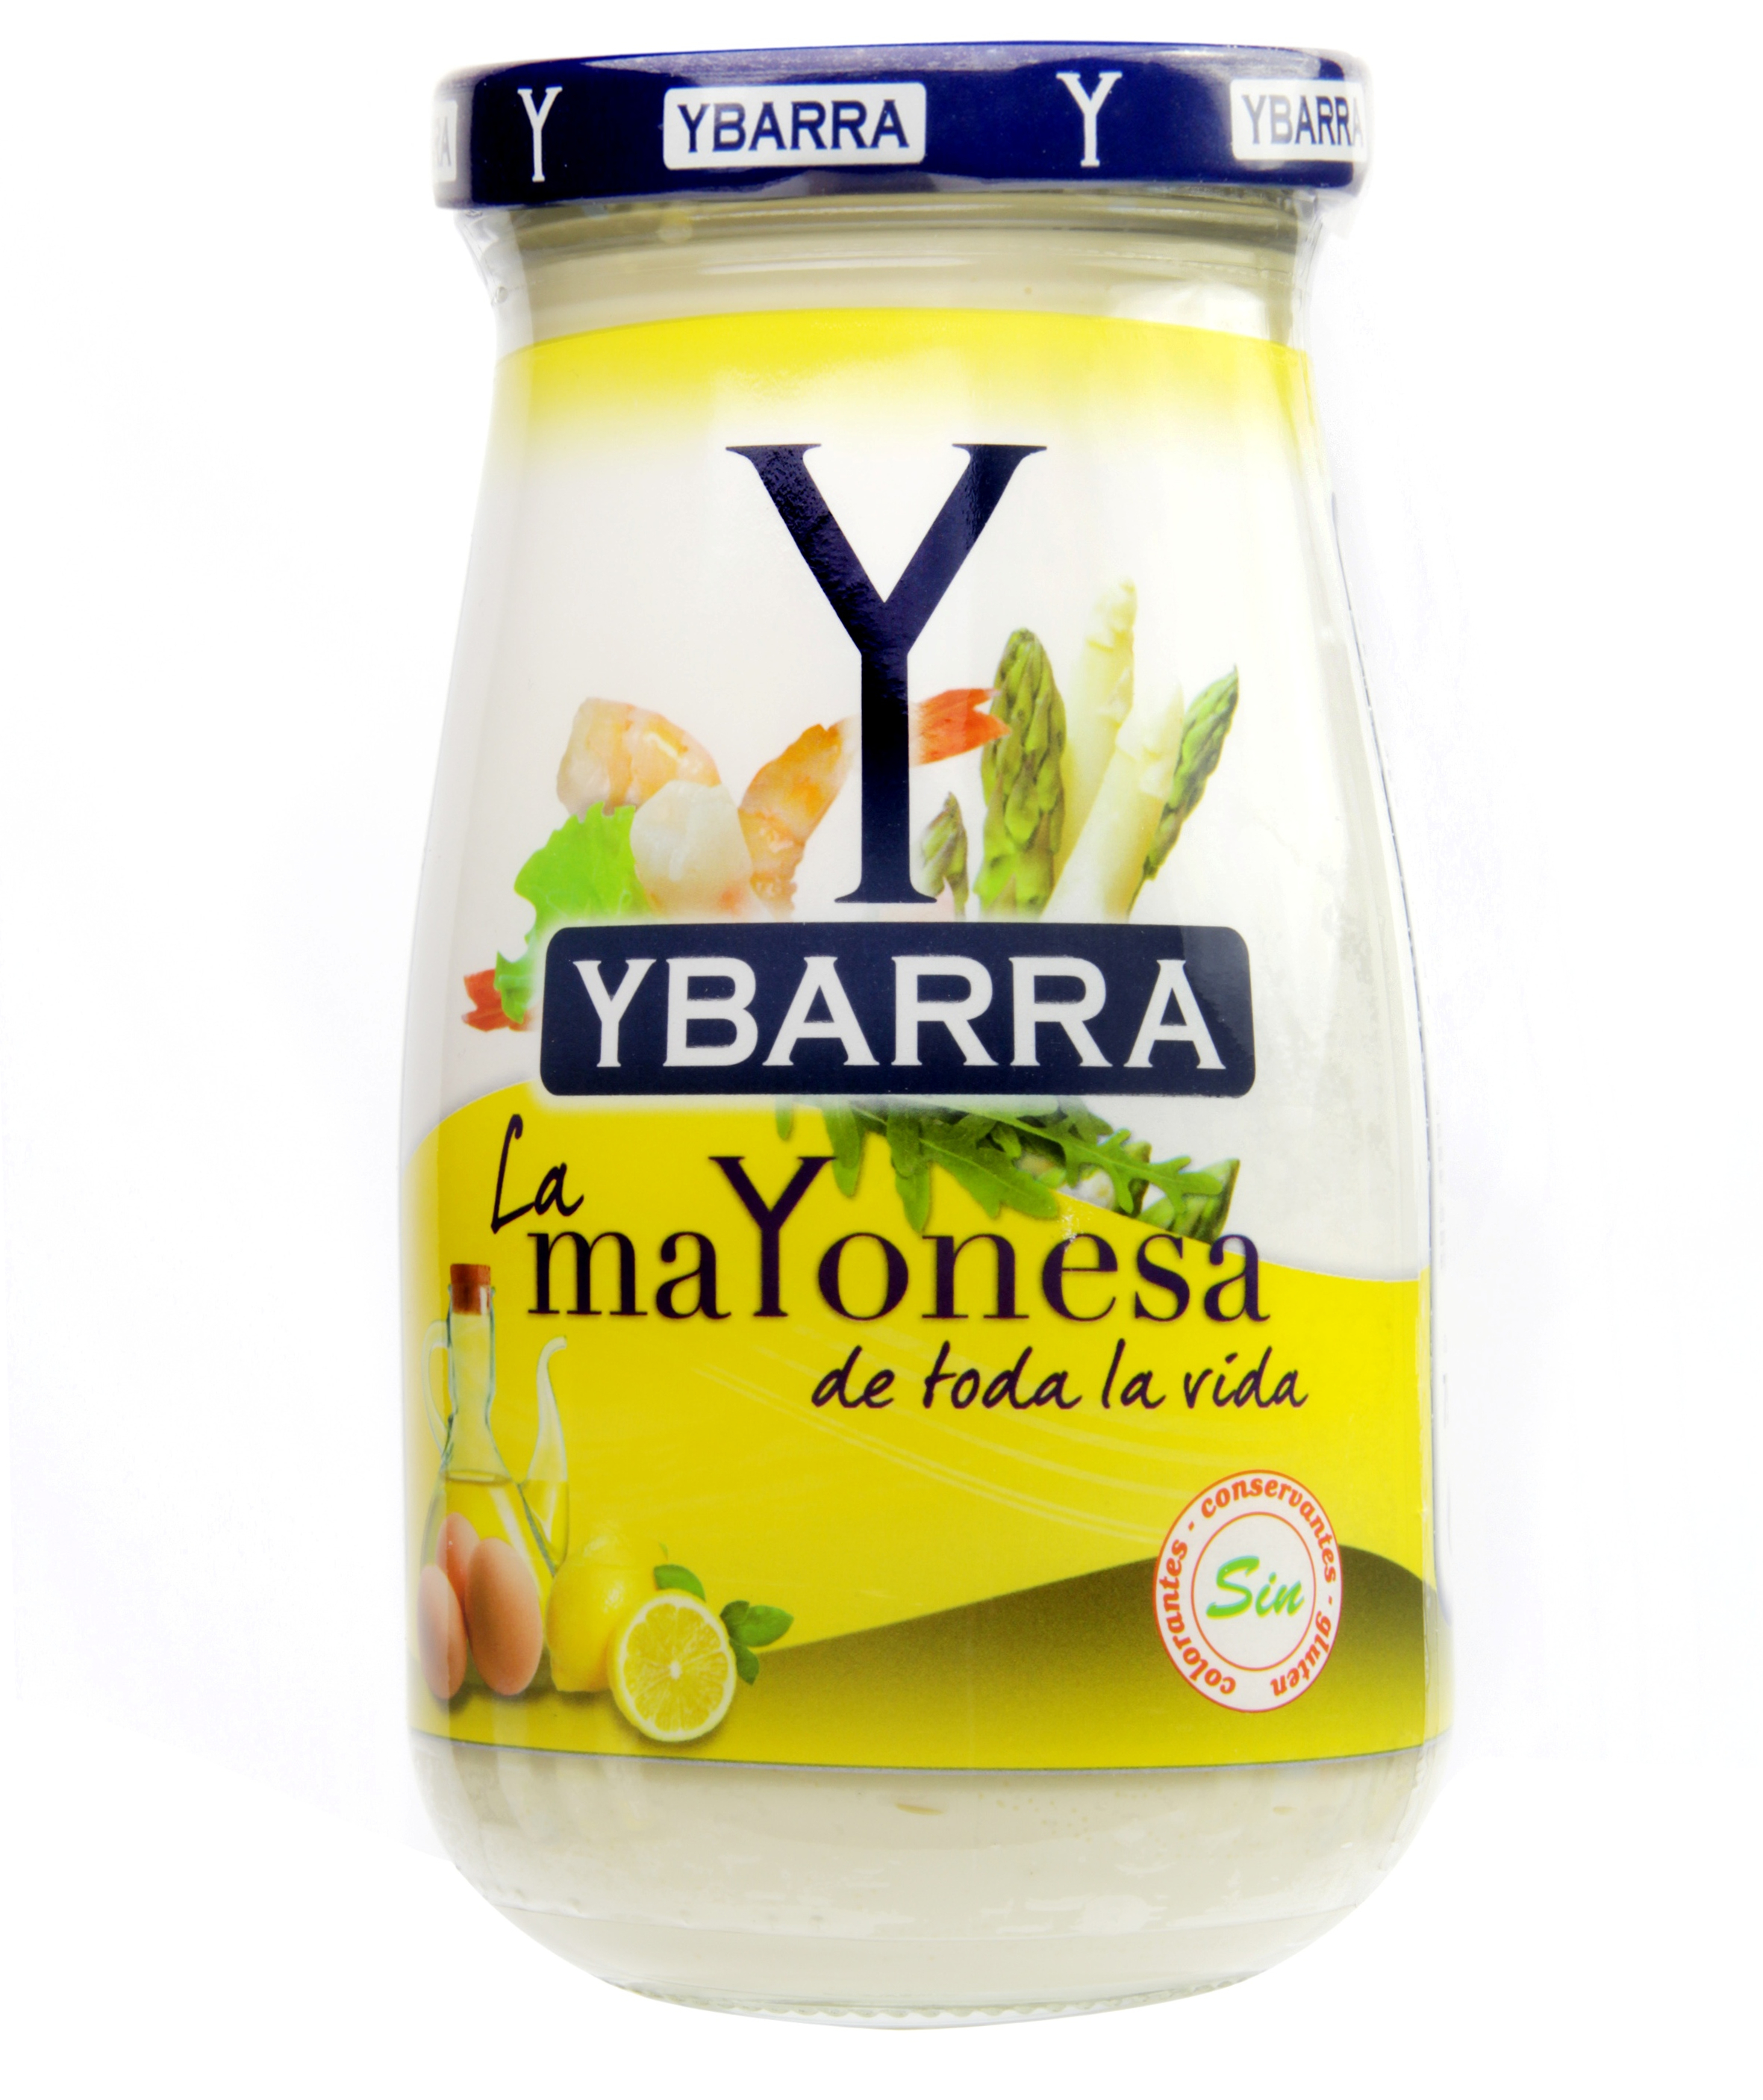
\includegraphics[width=0.6\textwidth]{figures/ybarra.jpg}
    \vfill
  \end{fullwidth}
\end{titlepage}

\tableofcontents

% ---- ----------------------------------------------------------
\newpage

\section{Meta stuff}

\textbf{Profesor:} Doctor Ricardo Ibarra García (\verb~ibarra@unizar.es~)

El examen (26930 Estado sólido II [T] 12 de la mañana: B-02, B-03) es un 70\%:
\begin{itemize}
\item Dos temas para desarrollar (se escoge uno, 30 min).
\item Dos ejercicios ya resueltos en clase, se elige uno (25\% de la
nota de examen, 30 min).
\item Tres cuestiones (20 min each) en las que no se puede elegir.
\end{itemize}
Los problemas de clase y la participación es el 20\%, y el 10\% son
son los informes de prácticas. Hay que sacar un 3 en \emph{todas} las partes.

Examen sorpresa en semana laica.

Las prácticas son en el INA, duran un par de tardes aproximadamente.

\subsection{Bibliografía}
\begin{itemize}
    \item Kittel.
    \item Ashcroft.
    \item Problemas del libro de problemas de Goldsmid.
      \verb|SL 57-144| (inglés), \verb|SL 60-40|, \verb|SL 1-154|
      (español).
    \item Blakemore para los dieléctricos (Solid State Physics).
    \item Blackey \& Blackey a veces.
\end{itemize}


\subsection{Estadística}
\marginnote[+1cm]{
  \begin{description}
  \item[The C thing]  3
  \item[The D thing]  4
  \item[The L thing]  62
  \item[The G thing]  4
  \end{description}
}
\begin{center}
  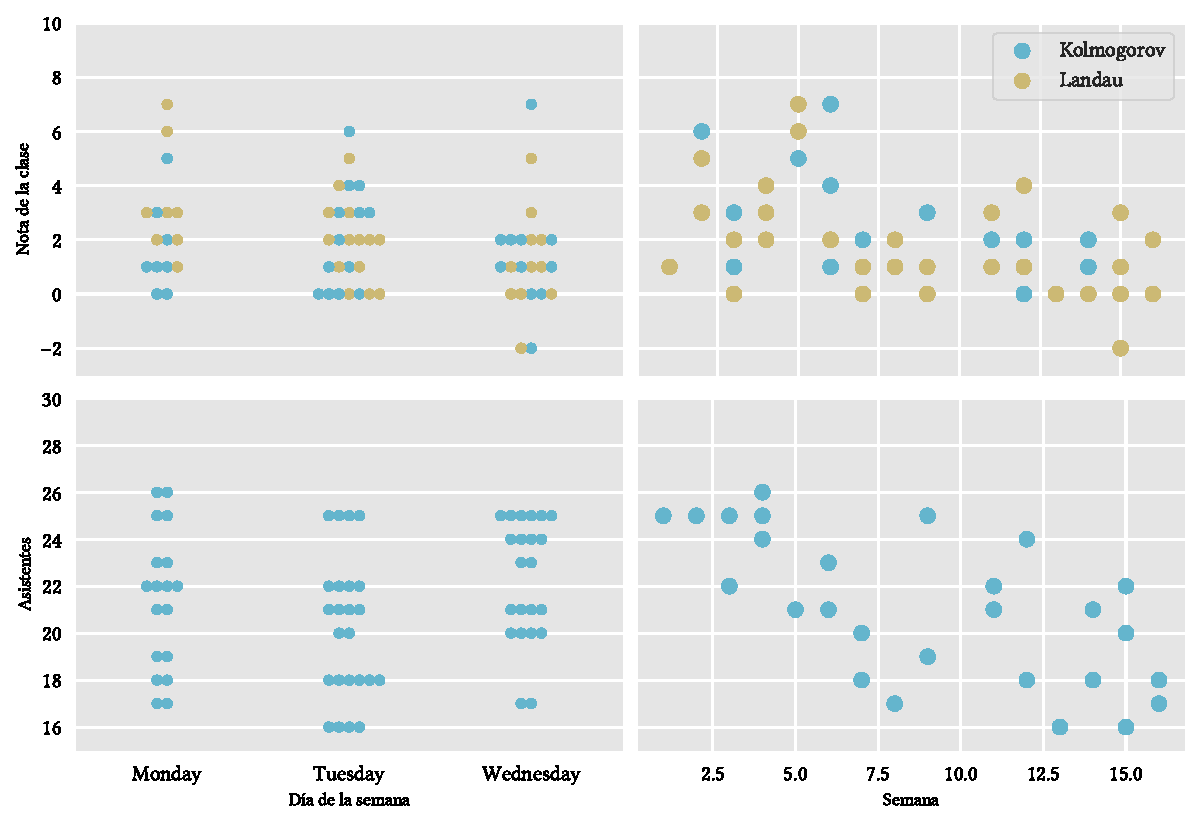
\includegraphics[width=\textwidth]{figures/metaplot.pdf}
\end{center}


%%%%%%%%%%%%%%%%%%%%%%%%%%%%
%
%   Temario:
%
%   1. Dieléctricos y ferroeléctricos.
%   2. Magnetismo de sólidos.
%   3. Superconductividad.
%   4. Sólidos nanoestructurados.
%   5. Sólidos amorfos.
%   6. Superficies, interfaces y multilayers.
%
%%%%%%%%%%%%%%%%%%%%%%%%%%%

\part{Teoría}
\chapter{Dieléctricos y ferroeléctricos}
%TL;DR: Band gap.

En los materiales dieléctricos, en lugar de cargas libres tenemos dipolos
eléctricos con momento dipolar total $\symbf{p}=\sum q_i\symbf{r}_i$ debido a
la distribución no simétrica de las cargas. Cuando se aplica un campo externo
sobre el material, los dipolos generan un campo de sentido opuesto que
disminuye la magnitud del campo total dentro del material.

El campo dipolar viene dado por
\begin{equation}
   \symbf{E} = \frac{1}{4πε_0}\frac{3(\symbf{p}
    \cdot\symbf{r})\symbf{r}-r^2\symbf{p}}{r^5}
\end{equation}

Ciertas moléculas, como el O\textsubscript{2} , pueden exhibir momento dipolar
a pesar de tener una distribución simétrica de carga, mediante la aplicación de
un campo eléctrico.

Además de las ya conocidas ecuaciones de Maxwell, se emplearán las
\emph{relaciones constitutivas}:

\begin{align}
   \symbf{D} &= ε_0\symbf{E} +\symbf{P} \\
   \symbf{P} &= (ε_r-1)ε_0\symbf{E} = ε_0 χ E
\end{align}


\section{Campo eléctrico microscópico}
El campo eléctrico en un material viene dado por suma del campo
externo global $\symbf{E}_0$ y el campo microscópico local
$\symbf{e}(\symbf{r})$.

Como $\symbf{e}(\symbf{r})$ tiene fuertes fluctuaciones locales, se define un
campo local $\symbf{E}(\symbf{r}_0)$ sobre una escala mesoscópica,
típicamente la celda unidad:

\begin{equation}
   \symbf{E}(\symbf{r}_0) =
    \frac{1}{V_c}\int\symbf{e}(\symbf{r})\dd{V}
\end{equation}

A este campo lo llamamos \emph{campo eléctrico macroscópico}. Para hallar su
componente debida a la polarización $\symbf{P}$, utilizamos un teorema de
electroestática que establece una equivalencia completa entre una lámina de
dieléctrico de polarización $\symbf{P}$ con un volumen idéntico de densidad
superficial $σ=\hat{n}⋅\symbf{P}$. Empleando el teorema de Ostrogradsky, vemos
que el campo eléctrico $\symbf{E}_1$ debido a dicha $σ$ es

\begin{equation}
    E_1 = \frac{-\abs{σ}}{ε_0} = \frac{-P}{ε_0}
\end{equation}

A $\symbf{E}_1$ se le denota \emph{campo de despolarización}. El campo
macroscópico $\symbf{E}$ dentro del material es la suma de
$\symbf{E}_1$ y el campo externo $\symbf{E}_0$.

Para elipsoides, cilindros y discos, una polarización uniforme $\symbf{P} =
(P_x,P_y,P_z)^\mathit{T}$ crea un campo $\symbf{E}_1$ uniforme:
\begin{equation}
    \symbf{E}_1 = \frac{-1}{ε_0} \mqty(N_xP_x\\ N_yP_y\\ N_zP_z)
\end{equation}

donde $N_i$ son los \emph{factores de despolarización}. Sus valores dependen de
la geometría del material y suman $1$. Para una esfera valen $\nicefrac{1}{3}$
y para una lámina fina son nulos excepto en la dirección normal.

\section{Campo eléctrico local en un átomo}

Recordamos que $\symbf{E}_0$ es un campo externo aplicado al material
para polarizarlo. Descomponemos el campo eléctrico en un átomo del material en
un término externo ($\symbf{E}_0$) y el campo de los dipolos
($\symbf{E}_1+\symbf{E}_2+\symbf{E}_3$). Notamos que
\begin{equation}
    \symbf{E}_1 + \symbf{E}_2 + \symbf{E}_3 = \frac{1}{4πε_0} \sum
    \frac{3(\symbf{p}_i\cdot \symbf{r}_i)\symbf{r}_i-\symbf{r}_i^2
    \symbf{p}_i}{r_i^5}
\end{equation}

Seguimos el método que Lorentz usó, introduciendo el concepto de
\emph{cavidad} (figura \ref{fig:fourfields}); definimos una superficie imaginaria (preferiblemente
esférica\footnote{Ante la ignorancia, la esfera.}) dentro del sólido y centrada en el átomo de
interés:

\begin{description}
    \item $\symbf{E}_0$ es el campo externo aplicado.
    \item $\symbf{E}_1$ es el campo de despolarización, provocado por la
        densidad superficial de carga.
    \item $\symbf{E}_2$ es el \emph{campo de cavidad de Lorentz}. Viene
        descrito por la carga equivalente $σ$ de la polarización de los átomos
        en la cavidad. Para una cavidad esférica vale
        $\frac{1}{3ε_0}\symbf{P}$, de forma que en una muestra esférica
        $\symbf{E}_1+\symbf{E}_2=0$.
    \item $\symbf{E}_3$ es el campo creado por los átomos dentro del
        material, y el único término que depende de la estructura cristalina.
        Para una distribución cúbica de dipolos paralelos, es nulo.
\end{description}
\begin{marginfigure}
  \centering
  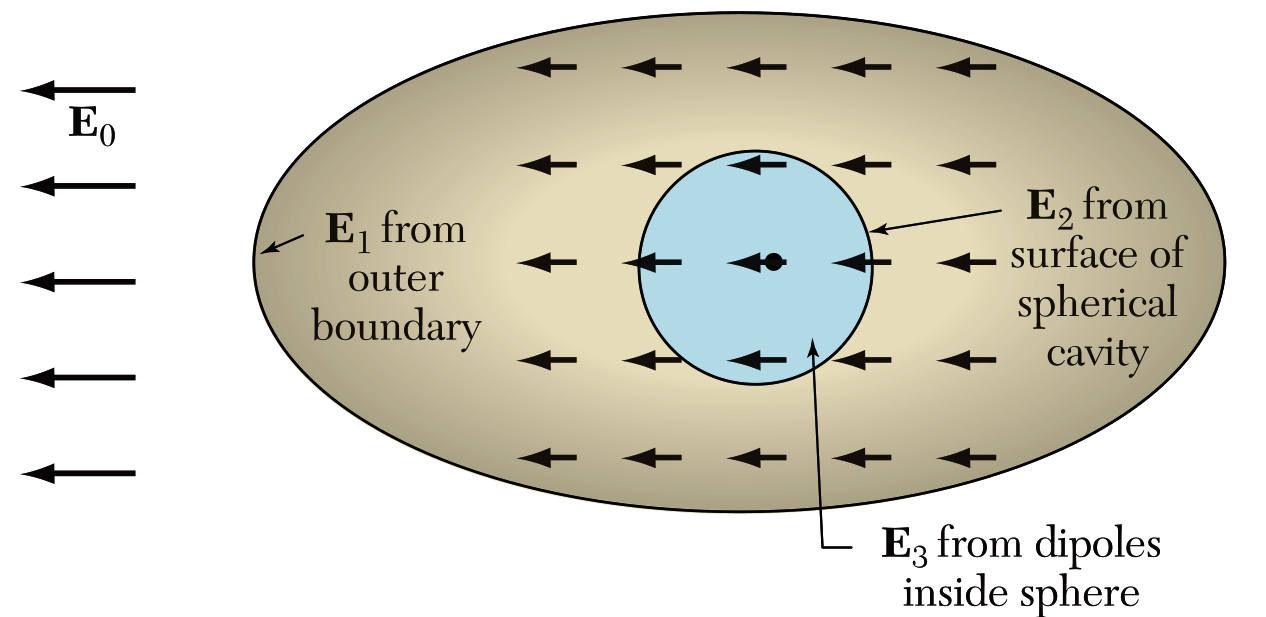
\includegraphics[width=\textwidth]{figures/fourfields.png}
  \caption{\itshape El campo eléctrico sobre un átomo es la suma de el
    campo externo $\symbf{E}_0$ y el campo de los demás átomos. A
    estos últimos los dividimos en una esfera de átomos locales con
    campo $\symbf{E}_3$ nulo en redes cúbicas
    (\textcolor{PlotDefault}{●}) y en una masa de dieléctrico
    uniformemente polarizada con campo $\symbf{E}_2+\symbf{E}_3$
    (\textcolor{PlotSecondary}{●}).}
  \label{fig:fourfields}
\end{marginfigure}


Notamos que $\symbf{E}_3$ es nulo para simetría cúbica. En tal caso, el campo
local será
\begin{equation}
    \symbf{E}_\mathit{local} = \underbrace{\symbf{E}_0
                               +\symbf{E}_1}_{\symbf{E}}
                               +\cancelto{\frac{\symbf{P}}{3ε_0}}{
                                   \symbf{E}_2}
                               +\cancelto{0}{\symbf{E}_3} = \symbf{E} +
                               \frac{1}{3ε_0} \symbf{P}
\end{equation}
donde se ha utilizado que el campo macroscópico $\symbf{E}$ viene definido por
$\symbf{E}_1+\symbf{E}_0$.

\section{Constante dieléctrica y polarizabilidad}
Se pueden relacionar mediante la relación de Clausius-Mossoti:
\begin{equation}
    \frac{ε-1}{ε+2} =  \frac{1}{3ε_0} \sum N_j α_j
\end{equation}
con $α$ la polarizabilidad eléctrica y $N$ las partículas por
metro cúbico. Notar como se relacionan magnitudes
microscópicas ($α$) con magnitudes macroscópicas (las $ε$).

\section{Origen de la polarizabilidad y respuesta a campo variable}

La contribución dipolar (u \emph{orientacional}) viene dada por dipolos
permanentes, como los del agua. Para mayores frecuencias (figura
\ref{fig:p_vs_f}), se produce un fenómeno de \emph{relajación}, donde los
dipolos permanentes no pueden seguir las rápidas variaciones del campo
eléctrico.
\begin{marginfigure}
    \centering
    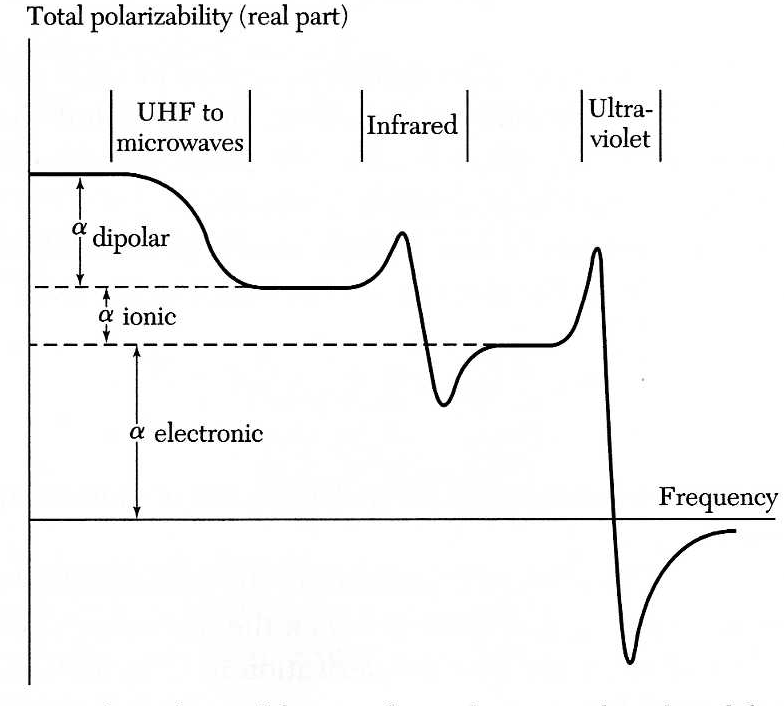
\includegraphics[width=\textwidth]{figures/polarizability_vs_freq.png}
    \caption{\itshape ``No está muy bien explicado, pero ya os imagináis lo que es.''}
    \label{fig:p_vs_f}
\end{marginfigure}
Los desplazamientos iónicos pasan a ser los relevantes. Por último,
en altas frecuencias, la única contribución relevante es la electrónica, ya que
los electrones son capaces de seguir el rápido campo eléctrico.


\subsection{Polarizabilidad electrónica}
En un modelo clásico, podemos considerar a los electrones ligados a los átomos
mediante muelles con frecuencia de resonancia $ω_0 = (β/m)^\oh$.

Bajo un campo eléctrico local, el desplazamiento viene dado por
\begin{equation}
    -e E_\mathit{loc} = βx = mω_0^2x
\end{equation}
La polarizabilidad estática será
\begin{equation}
    α_\mathit{electronic} = p / E_\mathit{loc} = -ex / E_\mathit{loc} =
    \frac{e^2}{mω_0^2}
\end{equation}

Resolviendo para un campo variable de frecuencia $ω$, obtenemos
\begin{equation}
    α_\mathit{electronic} = \frac{e^2 / m}{ω_0^2 - ω^2}
\end{equation}

En el rango visible se puede emplear la relación de Clausius-Mossoti; poniendo
$ε$ en función del índice de refracción $n$ se obtiene:

\begin{equation}
  α_\mathit{electronic} = \frac{3ε_0}{N_e} \frac{ε-1}{ε+2} =
  \frac{3ε_0}{N_e} \frac{n^2-1}{n^2+2}
\end{equation}

con $n$ el índice de refracción. Hay que notar que existe una
divergencia en $α$ que experimentalmente no se observa. La solución en
el modelo consiste en considerar unas pérdidas dieléctricas $mγ
\dv{x}{t}$.

\subsection{Polarizabilidad orientacional}

La energía de los dipolos depende de su ángulo con $\symbf{E}$,
\begin{equation}
    U = -\symbf{p}\cdot \symbf{E} = -pE \cos θ
\end{equation}

Al aplicar un campo se tendrá un $θ$ medio, de forma que $\symbf{P} =
Np\expval{\cos θ}$.  Notar como sin campo $\symbf{P} ∼ \expval{\cos θ} ∼ 0$.

Los dipolos se alinean en la dirección del campo, salvo por
pequeñas fluctuaciones térmicas. El ángulo puede describirse mediante una
estadística de Boltzmann:
\begin{equation}
    \expval{\cos θ} = \frac{\int e^{-βU}\cos θ \dd{Ω}}{\int
      e^{-βU} \dd{Ω}} = \coth (βpE) - \frac{1}{(βpE)} ≔ \text{L}(βpE)
\end{equation}

con $\text{L}(ζ)$ la \emph{función de Langevin}. Apróximándola a recta
(figura \ref{fig:langevin}) obtenemos la polarización por unidad de
volumen causada por reorientación de dipolos permanentes:
\begin{marginfigure}
    \centering
      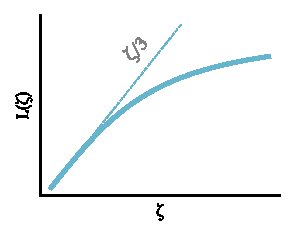
\includegraphics{figures/langevin.pdf}
    \caption{\itshape Función de Langevin. Para bajo $E$ puede aproximarse por
      $ζ/3$; valores de $E$ en los que esta aproximación deja de ser
      válida causan ruptura dieléctrica en muchos sólidos.}
    \label{fig:langevin}
\end{marginfigure}

\begin{equation}
  P = Np \underbrace{\expval{\cos θ}}_{≃ βpE/3} ≃ \frac{Np^2βE}{3}
\end{equation}

La polarización real, tal y como predice el modelo, aumenta con $β$ (y
disminuye con la temperatura), pero posee saltos discretos debido a
las limitaciones que impone la red en la orientación de los dipolos
(figura \ref{fig:jumps}).
\begin{marginfigure}
  \centering
    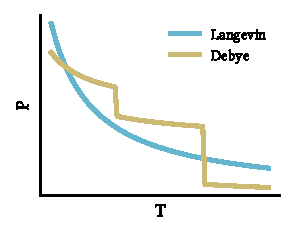
\includegraphics{figures/jumps.pdf}
    \caption{\itshape Polarización según los modelos de Debye y Langevin.}
  \label{fig:jumps}
\end{marginfigure}

Un modelo simple que explica este comportamiento es el de Debye.
Supongamos que hay dos $θ$ que minimizan la energía de una molécula
polar, $θ_1$ y $θ_2$, separadas por una barrera de potencial de altura
$Y$. La tasa de salto viene caracteriazada por una \emph{constante de
  relajamiento}:
\begin{equation}
  τ = \frac{1}{2πν\sub{D}} e^{βY}
\end{equation}

donde $ν\sub{D} ∼ \frac{\kb θ\sub{D}}{2π ℏ}$ es una frecuencia de
salto intrínseca del orden de \SI{1e12}{\hertz}, relacionada con el
límite superior del espectro de frecuencias vibracionales de la red.
De todas formas, si $Y$ es grande $\frac{1}{τ}$ no se parecerá a
\SI{1e-12}{\second}.

Un campo externo actuará sobre el doble pozo de potencial, haciendo un
estado (el de menor ángulo subtendido con el campo) más favorable.
Supuesto que se aplica el campo eléctrico durante un tiempo
suficientemente largo, se puede expresar la relación entre las
poblaciones en cada estado $θ_i$ como
\begin{equation}
  N_1 = N_2 \exp \left[ βpE(\cos θ_2 - \cos θ_1) \right]
\end{equation}
suponiendo una  distribución de Boltzmann y empleando
$U=-\symbf{p}\cdot \symbf{E}$.

Supongamos que ahora aplicamos un campo eléctrico de frecuencia
angular $ω$, suficientemente alta como para que los dipolos no tengan
suficiente tiempo como saltar de un estado a otro con normalidad ($ω ≳
\nicefrac{1}{τ}$) pero no tanto como para que no puedan seguir las
variaciones del campo. Como demostró\footnote{
  \emph{Polar molecules, chemical catalog Co. New York 1929, chap. V }}
Debye, la constante dieléctrica debe escribirse como una cantidad
compleja:
\begin{equation}
  ε = ε\sub{R} + iε\sub{I} = A + \frac{B}{1-iωτ} =
  \left( A + \frac{B}{1+ω^2τ^2} \right) + i \left( \frac{ωτB}{1+ω^2τ} \right)
\end{equation}

La polarización causada por dipolos inducidos (que no causa pérdidas
en este rango de frecuencias) está representada por $A$. A las
expresiones de  $ε\sub{R} , ε\sub{I}$ se les denota \emph{ecuaciones
  de Debye}. Puede verse una representación gráfica en la figura \ref{fig:debyeeq}.

\begin{marginfigure}
  \centering
    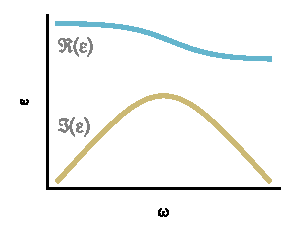
\includegraphics{figures/debyeeq.pdf}
  \caption{\itshape La parte imaginaria de la permitividad tiene un pico en
    $ω=\nicefrac{1}{τ}$. La gráfica está en escala logarítmica.}
  \label{fig:debyeeq}
\end{marginfigure}

\subsection{Polarizabilidad iónica}

Consideremos un sólido iónico con $N_e$ electrones polarizables por
centímetro cúbico y $N_i$ pares de iones polarizables. La ecuación de
Clausius-Mossoti relaciona $ε(ω)$ con las $α$:
\begin{equation}
  \frac{ε(0)-1}{ε(0)+2} = \frac{1}{3ε_0}(N_iα_i+N_eα_e)
\end{equation}

a bajas frecuencias. Para altas frecuencias, la constante dieléctrica
$ε(∞)$ depende solo de los $N_e$, ya que los iones no pueden
seguir la alta frecuencia:
\begin{equation}
  \frac{ε(∞) - 1}{ε(∞)+2} = \frac{1}{3ε_0} N_e α_e
\end{equation}

Restando ambas ecuaciones, podemos obtener la polarizabilidad iónica:
\begin{equation}
  α_i = \frac{3ε_0}{N_i} \left( \frac{ε(0)-1}{ε(0)+2} - \frac{ε(∞)-1}{ε(∞)+2} \right)
\end{equation}


\section{Piezoelectricidad}
Algunos materiales se polarizan al sufrir una deformación. Este efecto
este relacionado con simetrías cristalinas tal que no tienen centro de
inversión\footnote{
  Las estructuras que verifican que bajo un cambio de signo en las
  coordenadas no cambian tienen \emph{centro de inversión}. De los 32
  grupos puntuales, 21 carecen de él.
}; es fácil ver el origen de este comportamiento en una red con tres
dipolos a 120° (figura \ref{fig:dipole_120}). Pocos sólidos poseen un
efecto piezoeléctrico suficientemente grande como para ser medido.

\begin{figure}
  \centering
  \begin{tikzpicture}[>=stealth]
    \draw [->] (0,0) -- (+90:2);
    \draw [->] (0,0) -- (-30:2);
    \draw [->] (0,0) -- (-150:2);
    \node at (0,-2) {$\symbf{P}=0$};
  \end{tikzpicture}
  \qquad
  \begin{tikzpicture}[>=stealth]
    \draw [->] (0,0) -- (+90:2);
    \draw [->] (0,0) -- (-60:2);
    \draw [->] (0,0) -- (-120:2);
    \node at (0,-2) {$\symbf{P}=\ ↓$};
  \end{tikzpicture}
  \qquad
  \begin{tikzpicture}[>=stealth]
    \draw [->] (0,0) -- (+90:2);
    \draw [->] (0,0) -- (-15:2);
    \draw [->] (0,0) -- (-165:2);
    \node at (0,-2) {$\symbf{P}=\ ↑$};
  \end{tikzpicture}
  \caption{\itshape Una deformación modifica la suma vectorial de los tres
    dipolos, apareciendo un momento dipolar neto.}
  \label{fig:dipole_120}
\end{figure}


De manera equivalente, un campo eléctrico deforma los sólidos que
poseen esta propiedad. En primera aproximación, la deformación es
lineal con el campo eléctrico aplicado.

En cualquier sólido iónico, piezoeléctrico o no, existe un efecto
mucho menor denominado \emph{electroestricción}, que disminuye las
dimensiones del material de forma proporcional al \emph{cuadrado} del
campo aplicado.
\marginnote{\textcolor{gray}{¿Qué es morado y conmuta?\\ \emph{Una uva abeliana.}}}

\section{Ferroelectricidad}
En los sólidos ferroeléctricos el centro de cargas positivas y el de
negativas no coinciden incluso en ausencia de campo externo, de forma
que hay una polarización neta. Además de las restricciones en la
simetría discutidas al hablar de la piezoelectricidad\footnote{Todos
  los materiales ferroeléctricos son piezoeléctricos, pero lo
  contrario no es cierto.}, es necesario
que el cristal tenga una única dirección no equivalente.

\subsection{Ley de Curie-Weiss}

El comportamiento desaparece a temperaturas superiores a $T\sub{C}$, la
\emph{temperatura de Curie}. Por encima, el sólido se denota \emph{paraeléctrico}.

\marginnote{A los materiales cuyo momento dipolar cambia con la
temperatura debido a cambios conformacionales se les denota
\emph{piroeléctricos}. Son un subconjunto de los piezoeléctricos:
  \begin{center}
    \begin{tikzpicture}[xscale=1.5]
      \definecolor{A}{HTML}{FBDED0}
      \definecolor{B}{HTML}{DCEAB7}
      \definecolor{C}{HTML}{CCDDF1}
      \definecolor{bA}{HTML}{F26F52}
      \definecolor{bB}{HTML}{9CCE78}
      \definecolor{bC}{HTML}{3A99D4}
      \draw[bA, rounded corners,fill=A] (0,0) rectangle (3,2);
      \draw[bB, rounded corners,fill=B] (0,0) rectangle (2,1.5);
      \draw[bC, rounded corners,fill=C] (0.25,0.25) rectangle (1.75,1);
      \node[black] at (1.5,1.75) {\scshape Piezoeléctricos};
      \node[black] at (1,1.25) {\scshape Piroeléctricos};
      \node[black] at (1,0.625) {\scshape  Ferroeléctricos};
    \end{tikzpicture}
  \end{center}
}

Cerca de $T\sub{C}$, la susceptibilidad del material viene descrita
por una variación de la \emph{ley de Curie-Weiss}:
\begin{equation}
  χ = \frac{C}{T-θ}
\end{equation}
donde $θ$ es la \emph{constante de Weiss}. Cuando coincide con la
temperatura de Curie hay una transición de segundo orden con $χ^{-1}$
continua; en cualquier otro caso la transición es de primer orden con
discontinuidad en la inversa de la susceptibilidad.

Se muestra a continuación una representación gráfica de los
observables para una transición de primer orden
(\textcolor{PlotDefault}{●}) y de segundo (\textcolor{PlotSecondary}{●}).

\begin{fullwidth}
  \begin{center}
    % First order, Ps
    \begin{tikzpicture}
      \draw[->] (0,0) -- (3,0) node[below right] {$T$};
      \draw[->] (0,0) -- (0,3) node[above left] {$P\sub{S}$};
      \draw[PlotDefault, thick] (0,2) to[out=0, in=120] (2,1);
      \draw[PlotDefault, thick] (2,1) -- (2,0) node[below, black] {$T\sub{C}$};
      \node at (1,1) {\sansfont{{\scshape Ferro}}};
      \node at (2.5,2) {\sansfont{{\scshape Para}}};
    \end{tikzpicture}
    % First order, 1/χ
    \begin{tikzpicture}
      \draw[->] (0,0) -- (3,0) node[below right] {$T$};
      \draw[->] (0,0) -- (0,3) node[above left] {$1/χ$};
      \draw[PlotDefault, thick] (0,2.5) to[out=-20, in=140] (2,1.5);
      \draw[PlotDefault, dashed] (2,1.5) -- (2,0) node[below, black] {$T\sub{C}$};
      \draw[PlotDefault, dashed] (1,0) -- (2,1) node [black, at start, below] {$θ$};
      \draw[PlotDefault, thick] (2,1) -- (3,2);
      \node at (1,1) {\sansfont{{\scshape Ferro}}};
      \node at (2.3,2.2) {\sansfont{{\scshape Para}}};
    \end{tikzpicture}
    % First order, Ps
    \begin{tikzpicture}
      \draw[->] (0,0) -- (3,0) node[below right] {$T$};
      \draw[->] (0,0) -- (0,3) node[above left] {$P\sub{S}$};
      \draw[PlotSecondary, thick] (0,2) to[out=0, in=90] (2,0)
       node[below, black] {$T\sub{C}$};
      \node at (0.75,1) {\sansfont{{\scshape Ferro}}};
      \node at (2,2) {\sansfont{{\scshape Para}}};
    \end{tikzpicture}
    % First order, 1/χ
    \begin{tikzpicture}
      \draw[->] (0,0) -- (3,0) node[below right] {$T$};
      \draw[->] (0,0) -- (0,3) node[above left] {$1/χ$};
      \draw[PlotSecondary, thick] (0,2.5) -- (2,0)
       node[below, black] {$T\sub{C}=θ$};
      \draw[PlotSecondary, thick] (2,0) -- (3,2);
      \node at (0.75,0.5) {\sansfont{{\scshape Ferro}}};
      \node at (2.75,0.5) {\sansfont{{\scshape Para}}};
    \end{tikzpicture}
  \end{center}
\end{fullwidth}

\subsection{Dominios ferroeléctricos}
En un material ferroeléctrico sin campo aplicado, no todos los dipolos
apuntan en la misma dirección. En lugar de ello, se crean
\emph{dominios ferroeléctricos}: el material se subdivide en dominios,
en los cuales todos los dipolos están alineados, pero no
necesariamente todos los dominios tienen $\symbf{P}$ en la misma
dirección. Por ello, la $\symbf{P}$ total del material es nula.

Cuando aplicamos un campo eléctrico\footnote{El campo mínimo necesario
para que aparezca una polarización global se denota \emph{campo
coercitivo}.}, las $\symbf{P}$ colineares con él pasan a ser
favorables energéticamente, de forma que se rompe la simetría
rotacional de los dominios y se alinean en una dirección preferente.

Al quitar el campo eléctrico, queda una polarización residual llamada
\emph{polarización remanente}, que genera fenómenos de histéresis.

\section{Transición ferroeléctrica}
Se puede ver la transción de fase de los materiales desde dos puntos
de vista, uno microscópico y otro macroscópico.

\subsection{\textit{Polarization Catastrophe}: enfoque macroscópico}
En una \textit{polarization catastrophe} el campo eléctrico local
causado por el desplazamiento iónico es mayor que la fuerza de
recuperación, creando una variación asimétrica de las posiciones de
los iones. La polarización o alguna componente de Fourier suya se
vuelve muy grande.

Para hallar un modelo analítico, partimos de la ecuación de
Clausius-Mossoti. Si despejamos $ε$, obtenemos
\begin{equation}
  ε = \frac{1 + \frac{2}{3ε_0} \sum_{} N_i α_i }{1 - \frac{1}{3ε_0} \sum_{} N_i α_i }
\end{equation}
\marginnote{
  Se recuerda que $α_i$ es la suma de la polarizabilidad iónica y
  electrónica para un ion de tipo $i$ y $N_i$ es el número de estos
  iones por unidad de volumen.}

Inmediatamente notamos que $ε$ se vuelve infinita y permite
polarización finita con campo aplicado cero si $\sum_{} N_i α_i =
3ε_0$. El valor de $ε$ es extremadamente sensible a fluctuaciones
alrededor de este valor; definamos $\frac{1}{3ε_0} \sum_{} N_i α_i =
1-3s$, con $s$ muy pequeño. Obtenemos

\begin{equation}
  ε = \frac{1- 2s}{s} ≃ \frac{1}{s}
\end{equation}

Supongamos que cerca de la temperatura crítica $s$ es proporcional a
la temperatura como $s=(T-T\sub{C})/ξ$ con $ξ$ constante, obtenemos
\begin{equation}
  ε ≃ \frac{ξ}{T-T\sub{C}}
\end{equation}
Que ajusta bien los datos experimentales para $ε$ en la fase paraeléctrica.

\subsection{\textit{Phonon mode softening}: enfoque microscópico}

Partimos de la ecuación de Lyddane-Sachs-Teller, que permite
relacionar las $ω$ de los fonones de los modos longitudinales y
transversales con las constantes dieléctricas del material:
\begin{equation}
  \frac{ω\sub{T}^2}{ω\sub{L}^2} = \frac{ε(∞)}{ε(0)}
\end{equation}
Vemos que cuando $ω\sub{T}$ adquiere valores muy bajos, la
susceptibilidad estática $ε(0)$ puede diverger.

Si $1/ε(0) ∝ (T-T_0)$, se tiene que $ω^2\sub{T} = 1/ε(0) ∝ T$ supuesto
que $ω\sub{L}$ no depende de la temperatura. La
evidencia experimental confirma esta relación con excelente precisión.

\begin{marginfigure}
  \centering
  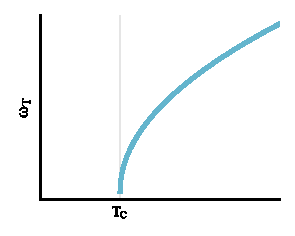
\includegraphics{figures/softphonon.pdf}
  \caption{\itshape Un estudio de los fonones del material predice que
    $ω\sub{T}^2 ∝ T$, anulándose en la temperatura de transición
    ferroeléctrica $T\sub{C}$.}
  \label{fig:softphonon}
\end{marginfigure}






% Tue Feb 28 08:31:28 CET 2017
\section{Teoría de Landau de las transiciones de fase}
Veremos que el parámetro de orden en la transición ferroeléctrica es
la polarización $\symbf{P}$.
% Eat Kittel
La energía libre $F(P,T,E)$ de un sistema dieléctrico se escribe en
términos de la polarización, la energía y la temperatura. En la teoría
de Landau, se omiten las potencias impares de la
polarización\footnote{ Se omiten para garantizar la reversibilidad
  temporal del sistema. Hay cristales en los que son relevantes, y sus
  transiciones no son clasificables como de primer o segundo orden.}
salvo $EP$:
\begin{equation}
  F(P,T,E) = -EP + g_0 + \frac{1}{2} g_2 P^2 + \frac{1}{4} g_4 P^4 + ⋯
\end{equation}
donde los coeficientes $g_i$ dependen de la temperatura. Para ver el
valor en equilibrio, se calcula $\dv{}{P} F = 0$, de forma que
obtenemos
\begin{equation}
  0 = -E + g_2 P + g_4 P^3 + g_6 P^5 + ⋯
\end{equation}
Ponemos $E$, el campo aplicado, despreciando el campo de
despolarización, y trabajamos en una sola dimensión.

Landau definió $g_2 = γ(T-T_0)$ con $γ=\text{cte.}$ y la posibilidad
de que $g_2$ sea negativo.

Si $g_4$ es positivo y con la definición anterior de $g_2$, al
calcular el mínimo con $E=0$ obtenemos
\begin{equation}
  γ(T-T_0) P\sub{S} + g_4 P_S^3 = 0
\end{equation}

Hay dos soluciones, $P\sub{S}=0$ y
\begin{equation}
  P_S^2 = \frac{γ}{g_4}(T_0-T)
\end{equation}

Para $T≥T_0$ se tiene $P\sub{S}$ nulo, y para $T<T_0$ se obtiene
$\sqrt{\frac{γ}{g_4}(T_0-T)}$. Vemos que la transcion es de
segundo orden al ir $P$ a cero de forma continua.


Si $g_4 < 0$ en la expansión, tenemos que mantener $g_6 > 0$ para evitar
que $P\sub{S}$ diverja a $-∞$. La condición de equilibrio para $E=0$
queda como:
\begin{equation}
  γ(T-T_0) P\sub{S} - \abs{g_4} P\sub{S}^3 + g_6 P\sub{S}^5 = 0
\end{equation}
La solución trivial es $P\sub{S}=0$; si sacamos factor común
$P\sub{S}$ se obtiene
\begin{equation}
  γ(T-T_0)  - \abs{g_4} P\sub{S}^2 + g_6 P\sub{S}^4 = 0
\end{equation}
cuya solución tiene una forma funcional más complicada que en el
caso anterior (representada en la figura \ref{fig:landau}).
\begin{marginfigure}
  \centering
  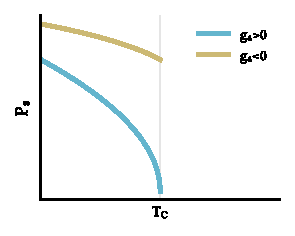
\includegraphics{figures/landau.pdf}
  \caption{\itshape Dependiendo del signo de $g_4$, la transición de fase es de
    primer o segundo orden.}
  \label{fig:landau}
\end{marginfigure}

% ⟨/dielectrics⟩
\chapter{Sólidos magnéticos}

La respuesta magnética de la materia bajo la aplicación de un campo
magnético depende de la existencia (o no) de un momento magnético
atómico. Desde un punto de vista clásico, un sistema en equilibrio
térmico no presenta momento magnético ni siquiera bajo la aplicación
de un campo (teorema de Bohr-van Leeuwen): el magnetismo es, por
tanto, inseparable de la mecánica cuántica.

El momento magnético de un átomo libre procede de tres fuentes: el
espín de los electrones, su momento angular orbital alrededor del
núcleo, y el cambio en el momento angular orbital inducido por un
campo magnético aplicado. Los dos primeros efectos aportan
contribuciones paramagnéticas a la magnetización, y el tercero aporta
una contribución diamagnética.

En el estado fundamental del átomo de hidrógeno, \textit{1s}, el
momento orbital es cero, y el momento magnético es el del espín
electrónico junto con un pequeño momento diamagnético inducido. En el
estado \textit{1s\textsuperscript{2}} del helio, tanto el espín como
el momento angular orbital son cero y sólo existe momento inducido.
Esto se puede generalizar: los átomos con con todas las capas
electrónicas llenas presentan $S = 0$ y $L = 0$, por lo que la
existencia de un momento magnético atómico se asocia con las capas
parcialmente llenas.



\section{Clasificación}

La magnetización $M$ se define como el momento magnético por unidad de
volumen, mientras que la susceptibilidad se define (en el vacío) como
$χ=\frac{M}{H}≃\frac{μ_0M}{B}$; esta última puede ser negativa en
materiales diamagnéticos.
\marginnote[-1cm]{
  Magnetización es un término completamente equivalente a imanación.
  La unidad de magnetización en CGS es el \textit{emu} por centímetro
  cúbico, equivalente a \SI{1e3}{\ampere\per\metre}.
}

Los materiales pueden clasificarse (figura \ref{fig:suschelp}) según
su $χ$ en \emph{ferromagnéticos}, \emph{paramagnéticos} y
\emph{diamagnéticos}.

\begin{marginfigure}
  \centering
  \begin{tikzpicture}
    \fill[PlotDefault] (0,0.25) rectangle (2,0.75) node[black, midway]
    {\scshape Ferro};
    \fill[PlotDefault] (0,1.25) rectangle (0.2,1.75);
    \node at (0.2,1.5) [right] {\scshape Para};
    \fill[PlotDefault] (0,2.25) rectangle (-0.1,2.75);
    \node at (0,2.5) [right] {\scshape Dia};
    \draw (0,3) -- (0,0);
    \draw[->] (0,3) -- (2,3) node [below] {$χ$};
  \end{tikzpicture}
  \caption{\itshape La susceptibilidad $χ$ ayuda a diferenciar las diferentes
    clases de materiales magnéticos.}
  \label{fig:suschelp}
\end{marginfigure}

\begin{description}
\item[Diamagnéticos]
  Experimentan una fuerza de repulsión ante un campo magnético, creando
  uno en la dirección opuesta.
  Todos los sólidos son diamagnéticos, incluso los que no tienen momento
  magnético permanente. Es un efecto muy tenue con origen en momentos
  magnéticos inducidos electromagnéticamente. Su principal
  característica es que $χ<0$ y muy pequeña ($\sim
  \SI{1e-5}{\emu\per\gram}$). Además, $χ$ no varía con la temperatura.

\item[Paramagnéticos]
  Se sienten atraídos por los campos magnéticos de forma débil. Se da
en sólidos con momento magnético permanente. $χ>0$ y va de
\SIrange{1e-5}{1e-3}{\emu\per\gram}, siendo dependiente de la
temperatura ($χ^{-1} ∝ T$).

  Más adelante se estudiarán las distintas contribuciones al efecto
  (figura \ref{fig:paramagnetic_contributions}).

  \begin{marginfigure}
    \centering
    \begin{tikzpicture}
      \draw[PlotDefault, thick] (0.5,2.5) to[out=-90,in=170]
      node[sloped,above,black] {Langevin} (3,0.75)
      ;
      \draw[PlotDefault, thick] (0,0.5) -- (3,0.5)
      node[midway, above, black] {Van Vleck}
      ;
      \draw[PlotDefault, thick] (0,0.2) -- (3,0.2)
      node[midway, black, fill=white] {Pauli}
      ;
      \draw[->] (0,0) -- (3,0) node[below] {$T$};
      \draw[->] (0,0) -- (0,3) node[right] {$χ$};
    \end{tikzpicture}
    \caption{\itshape El paramagnetismo tiene diversas fuentes, con diferentes
      orígenes y dependencias con la temperatura.}
    \label{fig:paramagnetic_contributions}
  \end{marginfigure}


\item[Ferromagnéticos]
  Se sienten atraídos fuertemente por campos magnéticos. Estos sólidos
  desarrollan interacciones de largo alcance por debajo de una
  temperatura crítica: \emph{es un fenómeno colectivo}. Como los
  ferroeléctricos, no muestran magnetización espontánea (en ausencia de
  campo) a pesar de tener dominios magnéticos por cancelarse entre
  ellos.
  \marginnote{Los únicos metales (puros) ferromagnéticos a temperatura ambiente
    son el hierro, el cobalto, el niquel, y el gadolinio.}
  Por debajo de la temperatura de transición son paramagnéticos.

\end{description}

Además de estos materiales existen dos tipos extra, relacionados con
los ferromagnéticos en el sentido de que están modelados por dipolos
permanentes en las posiciones de la red:

\begin{description}

\item[Antiferromagnéticos]
A diferencia de los ferromagnéticos, sus momentos dipolares alcanzan
la situación de mínima energía cuando se colocan de forma
antiparalela. Por ello, $M = \sum_{}m_i = M\sub{↑} + M\sub{↓} = 0$.

\item[Ferrimagnéticos]
  Son similares a los antiferromagnéticos, pero $M\sub{↑} ≠ M\sub{↓}$,
  de forma que $M ≠ 0$.

\end{description}

\begin{marginfigure}
  \centering
  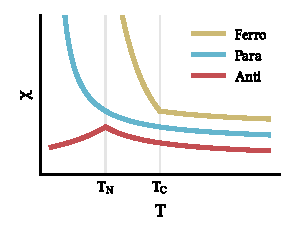
\includegraphics[width=\textwidth]{figures/chicomp.pdf}
  \caption{\itshape Tanto los materiales ferromagnéticos como los
    antiferromagnéticos son paramagnéticos por encima de las
    temperaturas de Curie y de Neel, respectivamente. En la fase
    paramagnética, $χ∼1/T$.}
  \label{fig:susc_comp}
\end{marginfigure}


\section{Diamagnetismo}
El diamagnetismo está asociado a la tendencia de las cargas eléctricas
a apantallar parcialmente al interior de un cuerpo de los campos
magnéticos externos. Los sólidos ``más diamagnéticos'' son los
superconductores, que apantallan completamente los campos magnéticos
externos (\emph{efecto Meissner}).

Se puede analizar desde un punto de vista
clásico\footnote{
Clásicamente, por el teorema de Bohr y Miss van-Leeuwen, el magnetismo
no puede existir en condiciones de equilibrio térmico. No obstante, se
supondrán \textit{ad hoc} órbitas estables que no irradian energía
para los electrones, posibilitándolo en un marco clásico.
}, con muy buenos resultados a pesar de las enormes
simplificaciones.

\subsection{Teoría clásica}
Suponemos que los electrones de los sólidos giran en órbitas clásicas
perfectamente circulares alrededor de los sólidos. En equilibrio,
\begin{equation}
  mω^2 r = \frac{1}{4πε_0} \frac{Ze^2}{r^2} + eωrB
\end{equation}
ya que el electrón experimenta una fuerza de Lorentz $\symbf{F} = e
(\symbf{v}× \symbf{B})$. Como en condiciones típicas de
laboratorio $\frac{eB}{2m} ≪ ω_0$,
\begin{equation}
  ω ≃ ω_0 + \frac{eB}{2m} = ω_0 + ω\sub{L}
\end{equation}
con $ω\sub{L}$ la \emph{frecuencia de Larmor}. La nueva $ω\sub{L}$
genera una corriente inducida extra, y por lo tanto un momento
magnético inducido debido al campo $\symbf{B}$.

El momento magnético de una espira de corriente es $μ=IS$. En este
caso (simetría esférica) $S=π(x^2+y^2)=\frac{2π}{3}\expval{r^2}$ e
\marginnote{
  \begin{equation*}
    \expval{x_i^2}+ \expval{y_i^2} = \frac{2}{3} \expval{r_i^2}
  \end{equation*}
}
$I=-Ze \frac{ω_L}{2π}$ (carga $×$ revoluciones $\div$ tiempo),
obteniendo $M=-Nμ$, lo que se traduce en
\begin{equation}
  χ ≃ \frac{μ_0M}{B} =  \frac{-μ_0NZe^2}{6m} \expval{r^2}
\end{equation}

\subsection{Teoría cuántica}
Asumamos un campo $\symbf{B} = \nabla × \symbf{A}$ uniforme.
El electrón experimentará\footnote{Alerta SI, se emplean unidades
  naturales con $ℏ=c=1$. Esto influye al la definición del momento
  generalizado (debería ser $e \symbf{A}/c$, no $e \symbf{A}$) y a
  $\mb = \frac{e ℏ}{2m_e}$ que queda como $\frac{e}{2m_e}$.}
un momento generalizado $\symbf{p} = m
\symbf{v} - e \symbf{A}$, de forma que
\begin{equation}
  \Ham = \frac{1}{2m} (\symbf{p} + e \symbf{A})^2 - e V
\end{equation}
Utilizando que $\symbf{B}$ es uniforme, se tiene $\symbf{A} =
\frac{1}{2} \symbf{B} × \symbf{r}$. Desarrollando el cuadrado del
hamiltoniano, se obtiene
\begin{equation}
  \begin{split}
    \Ham &= \frac{1}{2m} \left[ \symbf{p}^2 + 2e \symbf{p}\symbf{A}
      + e^2 \symbf{A}^2\right] - eV \\
    &=\frac{1}{2m} \left[ \symbf{p}^2 + e
      \symbf{p}(\symbf{B}×\symbf{r}) + \frac{e^2}{4}
      (\symbf{B}×\symbf{r})^2\right] - eV \\
    &=\frac{1}{2m} \left[ \symbf{p}^2 + e
      \symbf{B}(\underbrace{\symbf{r}×\symbf{p}}_{\symbf{ℓ}}) +
      \frac{e^2}{4} (\symbf{B}×\symbf{r})^2\right] - eV \\
    &= \frac{\symbf{p}^2}{2m} + \mb \symbf{B} \symbf{ℓ} +
    \frac{e^2}{8m} (\symbf{B}×\symbf{r})^2 - eV
  \end{split}
\end{equation}
\marginnote[-2cm]{
  El producto mixto es invariante ante permutaciones cíclicas:
  \begin{equation*}
      \symbf{A}⋅(\symbf{B}×\symbf{C})
    = \symbf{C}⋅(\symbf{B} × \symbf{A})
    = \symbf{B}⋅(\symbf{C} × \symbf{A})
  \end{equation*}
}

Para un átomo de $Z$ electrones,
\begin{equation}
  \Ham =
  \underbrace{
    \sum_{i=1}^Z \left( \frac{p_i^2}{2m} - eV(r_i) \right) +
    \sum_{i>j} \frac{e^2}{4πεr_{ij}} + λ \symbf{L} \symbf{S}
  }_{\Ham_0}
  +
  \underbrace{
    \mb \symbf{B} \left( \sum_{i=1}^Z \symbf{ℓ}_i + 2
      \sum_{i=1}^Z \symbf{s}_i \right) + \sum_{i=1}^Z
    \frac{e^2}{8m}(\symbf{B}×\symbf{r}_i)^2
  }_{\Ham'}
\end{equation}

donde $\Ham'$ es una perturbación sobre el hamiltoniano $\Ham_0$ de la
partícula libre. Podemos calcular la perturbación a primer orden $ΔE(B)$ en la
energía para una determinada función de ondas como
\begin{equation}
  \begin{split}
    ΔE(B) &= \mel{Ψ}{\Ham'}{Ψ} \\
    &= \mb \mel{Ψ}{\symbf{B}(\symbf{L}+2 \symbf{S})}{Ψ}
    + \frac{e^2}{8m} \mel{Ψ}{\sum_{i} (\symbf{B}× \symbf{r}_i)^2}{Ψ}
    \\
    &= \mb \mel{Ψ}{\symbf{B}(\symbf{L}+2 \symbf{S})}{Ψ}
    + \frac{e^2}{8m} B^2\sum_{i} \mel{Ψ}{x_i^2 + y_i^2}{Ψ}
    \\
  \end{split}
\end{equation}
donde se ha supuesto $\symbf{B}=B\hat{z}$.

Para el momento magnético, se obtiene
\begin{equation}
  \begin{split}
    \expval{μ_z} &= - \pdv{ΔE(B)}{B} = - \mb \expval{L_z + 2S_z}
    -
    \frac{e^2B}{4m} \expval{ \sum_{} (x_i^2+y_i^2)} \\
    &= μ_z^P + μ_z^d
  \end{split}
\end{equation}
A $μ_z^P$ se le denota \emph{momento magnético permanente} o
\emph{momento atómico} y a $μ_z^d$ \emph{momento magnético inducido}.
El primero es responsable del paramagnetismo y el segundo del
diamagnetismo; notar como sólo el segundo depende de $B$.
Cuando el átomo está completamente lleno, $μ_z^P=0$ y sólo queda el
segundo término.

Si suponemos simetría esférica,
$\expval{x_i^2}=\expval{y_i^2}=\expval{z_i^2}=\frac{1}{3}\expval{r_i^2}$
y
\begin{equation}
  χ_\mathit{diamag} ≃ \frac{μ_0N}{B}\expval{μ_z^d} = \frac{-μ_0e^2 N}{6m}
  \sum_{i=1}^Z \expval{r_i^2}
\end{equation}

Que es idéntica a la obtenida anteriormente mediante física clásica.

\section{Paramagnetismo}
\subsection{Teoría clásica}

La teoría clásica es idéntica a la de la paraelectricidad: suponemos
cada átomo como un pequeño dipolo magnético bajo fluctuaciones
térmicas.
\marginnote{En otros sistemas, como metales, este modelo del
clásico de paramagnetismo no es válido y se da otro tipo de paramagnetismo, que
se estudiará más adelante.}
Se tiene $U=- \symbf{μ} \symbf{B}$, considerando una
estadística de Maxwell-Boltzmann se obtiene
\begin{equation}
  \symbf{M} = Nμ \text{L}(βμB) \hat{B} ≃ \frac{βNμ^2 \symbf{B}}{3}
\end{equation}
con $\text{L}$ la \emph{función de Langevin}. La aproximación es
válida para $βμB ≪ 1$, y se denota \emph{ley de Curie}.
\marginnote{No confundir la ley de Curie-Weiss
  $ χ=\frac{C}{T-T\sub{C}} $
  con la ley de Curie
  $ \symbf{M} = C\frac{\symbf{B}}{T} $.
}


\subsection{Teoría cuántica}
La principal diferencia con la teoría clásica radica en la
cuantización de $μ$, de forma que $U$ deja de ser una distribución
estadística de valores continuos.
\marginnote{
  \begin{equation*}
    \mb = \frac{\displaystyle e ℏ}{\displaystyle 2m_ec}
  \end{equation*}
}
\begin{equation}
  \symbf{μ} = γ ℏ \ \symbf{J} = -g \mb \ \symbf{J}
\end{equation}
con $\symbf{J}$ el momento angular total (espín y orbital) y $γ$ el
\emph{factor giromagnético}, relacionado en un sistema electrónico con el
factor de \textit{splitting} espectroscópico $g$ (\emph{factor de Landé}).
\marginnote{Para electrones libres, $g≃2$. Para átomos libres,
  \begin{equation*}
    g = 1 + \frac{J(J+1) + S(S+1) - L(L+1)}{2J(J+1)}
  \end{equation*}
}
% Moar kittel

En un caso simple ($\symbf{L}=0$) sólo hay dos valores para el
\textit{splitting} de los niveles debido al momento magnético.

Tomando $μ=-g\mb S$ y teniendo en cuenta que $U =
-\symbf{μ}\symbf{B}$, aproximamos el sistema a un sistema clásico
para calcular las poblaciones de electrones con espín paralelo o
antiparalelo al campo obteniendo:
\begin{align}
  \frac{N_1}{N} &= \frac{e^{βμB}}{e^{βμB}+e^{-βμB}}\\
  \frac{N_2}{N} &= \frac{e^{-βμB}}{e^{βμB}+e^{-βμB}}
\end{align}
con $N_1$ la población con menor energía y $N_2$ la de mayor, ambas
separadas por $ΔE = 2μB$. Notar que se ha utilizado estadística de Boltzmann.

\begin{marginfigure}
  \centering
  \begin{tikzpicture}
    % Split
    \draw[thick, PlotDefault] (0,0) -- (1,0);
    \draw[thin, PlotDefault] (1,0) -- (1.25,1);
    \draw[thin, PlotDefault] (1,0) -- (1.25,-1);
    % Levels
    \draw[thick, PlotDefault] (1.25,1) -- (3,1)
    node[black, midway, fill=white] {$N_2$}
    node [black, right] {$m_s=\oh$};
    \draw[thick, PlotDefault] (1.25,-1) -- (3,-1)
    node[black, midway, fill=white] {$N_1$}
    node [black, right] {$m_s=\moh$};
    % Sep
    \draw[<->] (2.5,0.75) -- (2.5,-0.75) node[midway,fill=white] {$2μB$};
  \end{tikzpicture}
  \caption{\itshape Separación de los niveles atómicos para $L=0$. $J$
    sólo puede valer $±\oh$.}
  \label{fig:twolevelM}
\end{marginfigure}

Conforme se aumenta el campo $B$, aumenta $N_1$ y disminuye $N_2$.
Hallamos la magnetización como la suma de las poblaciones por su momento
magnético:
\begin{equation}
  M = (N_1 - N_2)μ = N μ \frac{e^{βμB} - e^{-βμB}}{e^{βμB} + e^{-βμB}}
  ≃ βNμ^2B
  \label{eq:simple}
\end{equation}
con la aproximación válida para $βμB ≪ 1$.

En el caso general ($\symbf{L}≠0$) se tienen $2J+1$ niveles
equiespaciados y una magnetización
\begin{equation}
  M = Nμ \text{B}_J(ζ)
\end{equation}
con $ζ=βμB$ y $\text{B}_J(ζ)$ la función de Brillouin (figura \ref{fig:brillouin}):
\begin{marginfigure}
  \centering
  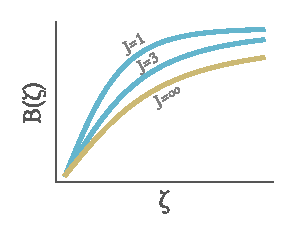
\includegraphics{figures/brillouin.pdf}
  \caption{\itshape La función de Brillouin converge a la de Langevin ($\coth x
    - 1/x$) para $J→∞$.}
  \label{fig:brillouin}
\end{marginfigure}
\begin{equation}
  \text{B}_J(ζ) = \frac{2J+1}{2J} \coth \frac{(2J+1)ζ}{2J} -
  \frac{1}{2J} \coth \frac{ζ}{2J}
\end{equation}

Para el caso especial $J=\oh$, se recupera \eqref{eq:simple}. La
susceptibilidad es inmediata de calcular como
\begin{equation}
  \frac{μ_0M}{B} = χ ≃ \frac{1}{3} μ_0βN(J+1)g^2μ^2\sub{B} = \frac{1}{3}
  βNp^2\mb^2 = \frac{C}{T}
  \label{eq:curielaw}
\end{equation}
donde $p=g\sqrt{J(J+1)}$ es el número efectivo de \emph{magnetones de
  Bohr} y $C$ es la \emph{constante de Curie}.


% <Start of chapa for Monday>
\subsection{Quenching orbital}
La expresión $p=g\sqrt{J(J+1)}$ no siempre predice bien las mediciones
experimentales, como pasa por ejemplo en el grupo del hierro. Si en
cambio se emplea $p=g\sqrt{S(S+1)}$ el parecido con los resultados
experimentales es notablemente mayor: es como si el momento angular orbital
$L$ no tuviera relevancia a la hora de calcular $J$.

Para entender este efecto, hay que considerar los efectos de un campo
cristalino no homogéneo $\symbf{E}$ en los átomos causado por los
iones del sólido.

\begin{itemize}
\item En primer lugar, puede separar niveles
atómicos degenerados. Este efecto, parecido al efecto Zeeman causado
por campos magnéticos, se denomina \emph{efecto Stark}.
\item En segundo lugar, el \textit{coupling} entre los vectores
  $\symbf{L},\symbf{S}$ se rompe, de forma que los autoestados del
  hamiltoniano ya no lo son de $\symbf{J}$, y no puede emplearse $J$
  únicamente para diferenciar estados.
\end{itemize}

Para sistemas de simetría ortorrómbica\footnote{Es similar a la cúbica, pero con un lado mayor que los demás.}
se tiene un potencial electroestático $φ$ de la forma
\begin{equation}
  eφ = Ax^2 + By^2 -(A+B)z^2
\end{equation}
tras solucionar\footnote{
  Es la solución de menor grado compatible con la simetría del
  sistema.
} la ecuación de Laplace $∇^2φ=0$. Si consideramos $ℓ=1$, se obtiene
que el estado fundamental está triplemente degenerado, y viene dado
por las funciones
\begin{equation}
  U_{x_i} = x_i f(r)
\end{equation}
con $x_i ∈\{x,y,z\}$. Si se asume que están normalizadas y son
ortogonales, puede comprobarse que cumplen
\begin{equation}
  \hat{L}^2 U_{x_i} = L(L+1) U_{x_i} = 2U_{x_i}
\end{equation}
donde $\hat{L}^2$ es el operador momento angular al cuadrado. Por lo
tanto, las $U_{x_i}$ corresponden a orbitales \textit{p}.

Notamos que la perturbación sobre los niveles causada por $eφ$ es nula
en los términos no diagonales $\mel{U_{x_i}}{eφ}{U_{x_j}},\ i≠j$,
debido a que aparecen funciones impares en las integrales.\footnote{
  Por ejemplo,
  \begin{equation*}
    \mel{U_x}{eφ}{U_y} = \int x y \abs{f(r)}^2 (Ax^2 + By^2 -
    (A-B)z^2) \dd{V}
  \end{equation*}
  Notar el término impar $xy$ multiplicando a términos pares.
}

Los términos diagonales no se anulan, y resultan:
\begin{equation}
  \begin{split}
    \mel{U_x}{eφ}{U_x} &= A(I_1-I_2) \\
    \mel{U_y}{eφ}{U_y} &= B(I_1-I_2) \\
    \mel{U_z}{eφ}{U_z} &= -(A+B)(I_1-I_2)
  \end{split}
\end{equation}
causando el desdoblamiento mostrado cualitativamente en la figura
\ref{fig:bananasplit}.

\begin{marginfigure}
  \centering
  \begin{tikzpicture}
    % Split
    \draw[thick, PlotDefault] (0,0) -- (1,0);
    \draw[thin, PlotDefault] (1,0) -- (1.25,1);
    \draw[thin, PlotDefault] (1,0) -- (1.25,-1);
    \draw[thin, PlotDefault] (1,0) -- (1.25,0.25);
    % Levels
    \draw[thick, PlotDefault] (1.25,1) -- (3,1)
    node[black, midway, fill=white] {\tiny $A(I_1-I_2)$}
    node [black, right] {$E_3$};
    \draw[thick, PlotDefault] (1.25,0.25) -- (3,0.25)
    node[black, midway, fill=white] {\tiny $B(I_1-I_2)$}
    node [black, right] {$E_2$};
    \draw[thick, PlotDefault] (1.25,-1) -- (3,-1)
    node[black, midway, fill=white] {\tiny $-(A+B)(I_1-I_2)$}
    node [black, right] {$E_1$};
  \end{tikzpicture}
  \caption{\itshape Un campo eléctrico inhomogéneo causado por el potencial
    cristalino causa un desdoblamiento de los niveles. Se muestra el
    efecto sobre un orbital $ℓ=1$ en simetría ortorómbica.}
  \label{fig:bananasplit}
\end{marginfigure}

El momento orbital de estos nuevos niveles es nulo, como se puede
comprobar sin más que calcular $\mel{U_{x_i}}{L_z}{U_{x_i}}$.\footnote{
  El operador momento angular viene dado por
  $\symbf{L}=\symbf{r}×\symbf{p} = \symbf{r}×(-i ℏ ∇)$:
  \begin{equation*}
    \symbf{L} = -i ℏ \mqty|
    \hat{i}   & \hat{j}   & \hat{k}   \\
    x         & y         & z         \\
    \pdv{}{x} & \pdv{}{y} & \pdv{}{z} \\
    |
    = -i ℏ \mqty(
    y \pdv{}{z} - z \pdv{}{y} \\
    -x \pdv{}{z} + z \pdv{}{x} \\
    x \pdv{}{y} - y \pdv{}{x} \\
    )
  \end{equation*}
  Luego $L_z$ es $-i ℏ\left(x \pdv{}{y} - y \pdv{}{x}\right)$. Es
  inmediato ver que los elementos de matriz con los $U_{x_i}$ se van a
  anular por quedar integrales de funciones impares.
}
A este efecto se le denota \emph{quenching}, el nivel todavía tiene un
momento angular definido al ser $\hat{L}^2$ diagonal y tener un
autovalor definido ($ℓ=1$), pero las componentes espaciales del
momento angular no son constantes del movimiento y su promedio
temporal se anula en primera aproximación.

En cristales que no tienen un $eφ$ cuadrático como el visto, como por
ejemplo los cúbicos, en principio los niveles no deberían separarse.
No obstante, la energía de los iones es más baja si se desplazan
respecto a su posición en la red, creando un potencial cuadrático como
el visto. Este desplazamiento espontáneo se denomina \emph{efecto
  Jahn-Teller} y suele ser importante y grande.

Podemos considerar la perturbación de la función de ondas $Ψ$ por el
acoplo espín-órbita $λ \symbf{L}\symbf{S}$. La variación en $E=g\mb H$
se traduce en una variación en $g$, el \emph{spectroscopic splitting
  factor}. En la dirección $\hat{z}$, se obtiene
\begin{equation}
  g = 2(1-λ/Δ_{xy})
\end{equation}
donde $Δ_{xy}$ corresponde a la diferencia de energía entre los orbitales
$p_x$ y $p_y$.

\subsection{Paramagnetismo de Van-Vleck}
En ocasiones, el $ΔE$ del desdoblamiento es del orden de la energía
térmica del sistema; ocurre por ejemplo en tierras raras.

Para obtener la contribución al paramagnetismo causada por esta
situación, consideramos un átomo o molécula que no tiene momento
magnético en el estado fundamental $\ket{0}$.

A pesar de que $\mel{0}{μ_z}{0}=0$, existe una contribución
mecanocuántica de niveles superiores, debida a términos perturbativos
$\mel{n}{μ_z}{0}$ de fuera de la diagonal. Los estados perturbados del
nivel fundamental y el excitado vendrán dados por
\begin{align}
  \ket{0'} &= \ket{0} + \frac{B}{ΔE} \mel{n}{μ_z}{0} \ket{n} \\
  \ket{n'} &= \ket{n} - \frac{B}{ΔE} \mel{0}{μ_z}{n} \ket{0}
\end{align}
con $ΔE = E_n - E_0$, diferencia de energías entre $\ket{n}$ y
$\ket{0}$, y $\mb B ≪ ΔE$. La contribución al paramagnetismo va a ser
pequeña al ser $ΔE$ grande, pero puede ser relevante si
$\mel{0}{μ_z}{0}∼0$.

El momento magnético del estado fundamental será
\begin{equation}
  \mel{0'}{μ_z}{0'} ≃ \frac{2B}{ΔE} \abs{\!  \mel{n}{μ_z}{0}  }^2
\end{equation}
y el del nivel superior
\begin{equation}
  \mel{s'}{μ_z}{s'} ≃ \frac{-2B}{ΔE} \abs{\!  \mel{n}{μ_z}{0}  }^2
\end{equation}
sin más que calcular los productos y despreciar los términos
$\order{ΔE^{-2}}$ y suponer $\mel{0}{μ_z}{0}∼0$.

Hay dos casos interesantes que considerar:
\begin{itemize}
\item Si $ΔE ≪ \kb T$, la población en el estado excitado es
  aproximadamente\footnote{
    Utilizando estadística de
    Boltzmann ($N e^{-βE}$) se obtenie
    \begin{equation*}
      \begin{split}
        N_\mathit{ground} -N_\mathit{excited} &= \frac{N}{2} e^{-βE_0}
        - \frac{N}{2} e^{-βE_s}
        \\
        &= \frac{N}{2}(1-βE_0) - \frac{N}{2}(1-βE_s)\\
        &= \frac{N}{2} β(E_s -E_0)
      \end{split}
    \end{equation*}
    donde $E_s$ es la energía del estado excitado y se ha empleado que
    $e^{x} ∼ 1+x$. Es tentador emplear $N$ en lugar de $N/2$, pero
    entonces la suma resultaría $2N$ en lugar de $N$.
  } $βNΔE/2$. La magnetización y
  susceptibilidad resultantes son
  \begin{align}
    M &= \expval{μ_z}N' = \frac{2B \abs{\!\mel{n}{μ_z}{0}}^2}{ΔE} \frac{βN ΔE}{2} \\
    χ &= βμ_0N \abs{\!\mel{n}{μ_z}{0}}^2
  \end{align}

  donde $N$ es el número de moléculas por unidad de volumen.
  La dependencia de $χ$ es similar a la ley de curie ($χ ∼ T^{-1}$)
  pero el mecanismo es completamente diferente.

\item Si $ΔE ≫ \kb T$, casi toda la población está en el nivel
  fundamental, y sólo este contribuye al paramagnetismo.
  \begin{align}
    M &= \expval{μ_z}N' = \frac{2B \abs{\!\mel{n}{μ_z}{0}}^2}{ΔE} N \\
    χ &= \frac{2Nμ_0 \abs{\!\mel{n}{μ_z}{0}}^2}{ΔE}
  \end{align}

  independiente de la temperatura. A esta contribución es a la
  que se le denota \emph{paramagnetismo de Van Vleck}.

\end{itemize}

Notar que si $ΔE$ aumenta, disminuye esta contribución a $χ ∼
ΔE^{-1}$. Por ello, los materiales con niveles energéticos poco
separados son más susceptibles de mostrar este efecto.

\subsection{Contribución electrónica}
Los espines de los electrones de conducción, con momento magnético
$\mb$, contribuyen al paramagnetismo. Cabría esperar que esta
contribución siguiera la ley de Curie-Weiss ($M=N
\mb^2B/\kb T$), pero se obtiene un valor astronómico que
no tiene nada que ver con la realidad. Experimentalmente se ve que
además la mayor parte del paramagnetismo no depende de la temperatura.

El fallo del enfoque está no tener en cuenta la estadística de
Fermi-Dirac. Los estados electrónicos por debajo del nivel de Fermi
están ocupados a $T=0$, y no hay posibilidad de pasar de espín
\textit{down} a espín \textit{up}.

Pauli supuso que sólo una fracción $∼T/T\sub{F}$ de los electrones
está a una energía $\kb T$ por encima del nivel de Fermi y tienen la
oportunidad de cambiar, contribuyendo a la susceptibilidad. Obtenemos
% Kittle
\begin{equation}
  M  ≃ N \frac{\mb^2 B}{\kb T}\frac{T}{T\sub{F}} =
  N\frac{\mb^2 B}{\kb T\sub{F}}
  \label{eq:cutre}
\end{equation}
que es independiente de $T$ y del orden de magnitud observado.

Con este nuevo planteamiento, tratamos de calcular la susceptibilidad
paramagnética de un gas de electrones libres de forma más rigurosa,
empleando la densidad de estados electrónicos (figura \ref{fig:dos}).

\begin{marginfigure}
  \centering
  \begin{tikzpicture}
    \fill[PlotDefault!20!white] (-1.5,2) to[out=-80, in=180]
    (0,-0.25) -- (0,2) ;
    \fill[PlotDefault!20!white] (1.5,2) to[out=-110, in=0] (0,0.25)
    -- (0,2);
    \fill[white] (-2,2) rectangle (2,1.5);
    \draw[thick, PlotDefault] (1.5,2) to[out=-110, in=0] (0,0.25);
    \draw[thick, PlotSecondary] (1.5,1.75) to[out=-110, in=0] (0,0);
    \draw[thick, PlotDefault] (-1.5,2) to[out=-80, in=180] (0,-0.25);
    \draw[] (-2,0) -- (2,0) node[at end, below] {DOS};
    \draw[] (0,-1) -- (0,3) node[at end, right] {$E$};
    \draw[dashed, gray, thin] (0,1.5) -- (2,1.5) node[at end, above] {$E\sub{F}$};
    \node at (-0.5,1) {$\ket*{↑}$};
    \node at (0.5,1) {$\ket*{↓}$};
    \draw[gray, thin] (0,0.25) -- (1,0.25) ;
    \draw[gray, thin] (0,-0.25) -- (1,-0.25) ;
    \draw[gray, thin, <->] (0.75,-0.25) -- (0.75,0.25) node[right,
    midway, fill=white, inner sep=0.5mm] {$2\mb B$};
  \end{tikzpicture}
  \caption{\itshape Un campo magnético desequilibra las densidades de
    estados, dando lugar a una magnetización neta en el material. Se
    muestra en amarillo (\textcolor{PlotSecondary}{●}) la densidad de
    estados $D(E)$ antes de aplicar el campo. Las otras
    (\textcolor{PlotDefault}{●}) curvas corresponden a $D(E±\mb B)$.}
  \label{fig:dos}
\end{marginfigure}

El número de electrones con momento magnético paralelo al campo
externo es
\begin{equation}
  N_+ = \frac{1}{2} \int_{-\mb B}^{E\sub{F}} D(E+\mb B) \dd{E}
  ≃ \frac{1}{2} \int_0^{E\sub{F}} D(E) \dd{E}+ \frac{1}{2} \mb B D(E_F)
\end{equation}
\marginnote{
  \begin{equation*}
    D(E) = \frac{1}{2π^2} \left( \frac{2m_e}{ℏ^2} \right)^{\nicefrac{3}{2}}
    \sqrt{E}
  \end{equation*}
}
donde se ha aproximado $\kb T ≪ E\sub{F}$ en $D(E) \propto \sqrt{E}$,
y se ha empleado $D(E+\mb B) ∝ \sqrt{E+\mb B}$ en lugar de $D(E) ∝ \sqrt{E}$ para
desplazar la densidad de estados y que quede como en la figura
\ref{fig:dos}.

El número de espines antiparalelos $N_-$ se calcula igual:
\begin{equation}
  N_- = \frac{1}{2} \int_{-\mb B}^{E\sub{F}} D(E-\mb B) \dd{E}
  ≃ \frac{1}{2} \int_0^{E\sub{F}} D(E) \dd{E}- \frac{1}{2} \mb B D(E_F)
\end{equation}

La magnetización viene dada por $M=\mb(N_+-N_-)$, de forma que
\marginnote{
  \begin{equation*}
    D(E\sub{F}) = \frac{3N}{2E\sub{F}}= \frac{3N}{2\kb T_F}
  \end{equation*}
}
\begin{equation}
  M = \mb ⋅ \mb B D(E\sub{F}) = \frac{3N\mb^2}{2\kb T_F} B
\end{equation}

Hay que notar que se ha ignorado la variación en las coordenadas
espaciales de los electrones debidas al campo magnético.
Landau\footnote{
  \vspace{-0.75cm}
  \begin{center}
    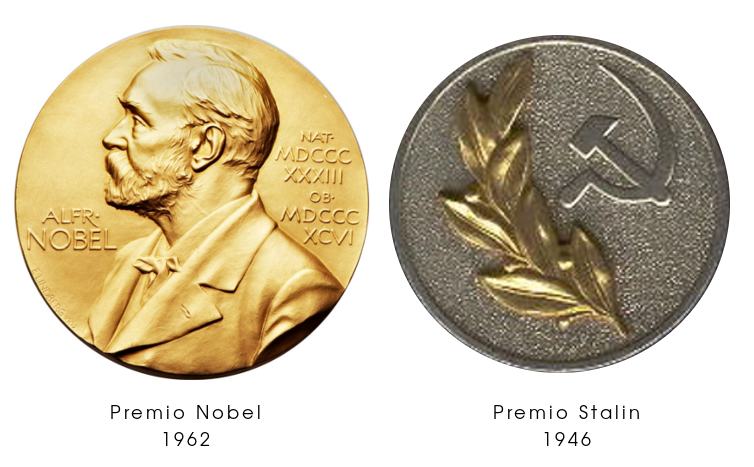
\includegraphics[width=0.5\textwidth]{figures/prizes.png}
  \end{center}
} mostró que el diamagnetismo causado por este efecto aporta un
$χ_\mathit{diam} = \nicefrac{-1}{3}χ_\mathit{Pauli}$, de forma que se
acaba obteniendo

\begin{equation}
  M = \mb D(E\sub{F})B = \frac{N\mb}{\kb T_F} B
\end{equation}

que es cualitativamente similar al resultado de \eqref{eq:cutre}

% New things:
\section{Ferromagnetismo}

\marginnote{\textcolor{gray}{Frotar un ajo contra un metal aumenta sus
propiedades magnéticas.}}


% Tue Mar 21 09:10:49 CET 2017

% Resumen del día anterior:

% Deberían seguir curie-weiss. Eso depende de T, pero experimentalmente
% no depende. Solución: multiplicar Curie-weiss por la fracción que sí
% que es capaz de girar. Ahora tenemos algo independiente de T.

% Suponemos que siguen std de Fermi Dirac, que cada e es independ y cada
% uno aporta μ=-μB. Prop de espines alineados con B: N+. (kbT ≪ Ef para
% que puedan flipar). Igual con N- (antiparalelos). Desarrollamos ambas
% en series de ε. M=μ(N+ - N-) ≠ f(T).

% Esto sólo es ef paramagnético. Landau demostró que χ diamagnética es
% ⅓ de diamagnética (o paramag o algo, mirar).

% Gráfica de paraboloide montado en ΔE, separación 2μB.

% Día de ejercicios (because).
% Bye.

% Biblio para siguiente clase: COEY: magnetism and magnetic materials.

La diferencia de estos materiales con los diamagnéticos y paramagnéticos es la aparición
de una imanación espontánea aun en la ausencia de campo externo. Esta
se debe a interacciones de largo alcance.

Existen distintas clases de materiales con este comportamiento:
\begin{description}
\item[Ferromagnéticos]
  \begin{tikzpicture}[xscale=0.2, yscale=0.4]
    \draw[->, >=stealth'] (0,0) -- (0,1);
    \draw[->, >=stealth'] (1,0) -- (1,1);
    \draw[->, >=stealth'] (2,0) -- (2,1);
    \draw[->, >=stealth'] (3,0) -- (3,1);
    \draw[->, >=stealth'] (4,0) -- (4,1);
  \end{tikzpicture}
  \quad
  Los momentos magnéticos están alineados, dando una magnetización neta.
\item[Antiferromagnéticos]
  \begin{tikzpicture}[xscale=0.2, yscale=0.4]
    \draw[->, >=stealth'] (0,0) -- (0,1);
    \draw[->, >=stealth'] (1,1) -- (1,0);
    \draw[->, >=stealth'] (2,0) -- (2,1);
    \draw[->, >=stealth'] (3,1) -- (3,0);
    \draw[->, >=stealth'] (4,0) -- (4,1);
  \end{tikzpicture}
  \quad
  Los espines están desalineados, de forma que no hay magnetización
  neta. No obstante, hay interacción de largo alcance.
\item[Ferrimagnéticos]
  \begin{tikzpicture}[xscale=0.2, yscale=0.4]
    \draw[->, >=stealth'] (0,0) -- (0,0.75);
    \draw[->, >=stealth'] (1,1) -- (1,0);
    \draw[->, >=stealth'] (2,0) -- (2,0.75);
    \draw[->, >=stealth'] (3,1) -- (3,0);
    \draw[->, >=stealth'] (4,0) -- (4,0.75);
  \end{tikzpicture}
  \quad $M_↑ \neq M_↓$, creando una magnetización neta.
\item[Canted ferromagnets]
  \begin{tikzpicture}[xscale=0.2, yscale=0.4]
    \draw[->, >=stealth'] (0,0) -- (0.3,1);
    \draw[->, >=stealth'] (1,1) -- (1.3,0);
    \draw[->, >=stealth'] (2,0) -- (2.3,1);
    \draw[->, >=stealth'] (3,1) -- (3.3,0);
    \draw[->, >=stealth'] (4,0) -- (4.3,1);
  \end{tikzpicture}
  \quad
  Suele ser un magnetismo débil. En el ejemplo dibujado, la red posee
  una $M$ no nula en $\hat{x}$ por no estar perfectamente alineada.
\item[Helical ferromagnets]
  \begin{tikzpicture}[xscale=0.2, yscale=0.4]
    \draw[gray] (0,0) -- (1,1);
    \draw[gray] (0,0) -- (1,-1);
    \draw[gray, fill=white] (1,0) ellipse (0.4 and 1);
    \draw[->, >=stealth'] (0,0) -- (1,1);

    \draw[gray] (2,0) -- (3,1);
    \draw[gray] (2,0) -- (3,-1);
    \draw[gray, fill=white] (3,0) ellipse (0.4 and 1);
    \draw[->, >=stealth'] (2,0) -- (3.35,0.6);

    \draw[gray] (4,0) -- (5,1);
    \draw[gray] (4,0) -- (5,-1);
    \draw[gray, fill=white] (5,0) ellipse (0.4 and 1);
    \draw[->, >=stealth'] (4,0) -- (5.4,0.25);

    \draw[gray] (6,0) -- (7,1);
    \draw[gray] (6,0) -- (7,-1);
    \draw[gray, fill=white] (7,0) ellipse (0.4 and 1);
    \draw[->, >=stealth'] (6,0) -- (7.4,-0.5);
  \end{tikzpicture}
  \quad
  Típico de los lantánidos. Como en los demás tipos de
materiales vistos hay una periodicidad de largo alcance, por ejemplo
cada 15 o 20 átomos. Nuevamente, el ejemplo dibujado posee una
magnetización en $\hat{x}$.
\end{description}

La imanación de los materiales ferromagnéticos es órdenes de magnitud
mayor a la de paramagnéticos y diamagnéticos, aun con campos mucho
menores. La imanación remanente máxima a la que llegan se denota
\emph{imanación de saturación}.



Podríamos suponer que el ferromagnetismo está basado en interacciones
dipolares magnéticas, pero un cálculo rápido muestra que la hipótesis
no es compatible con las energías implicadas en el fenómeno.
Un momento magnético tiene una energía $U$ por estar en el campo dipolar
magnético de otro momento:
\begin{equation}
  U = \frac{\symbf{m}_1 \symbf{m}_2 - 3(\symbf{m}_1
  \hat{r}) (\symbf{m}_2\hat{r})}{r^3}
\end{equation}

Supuesto $m_1≃m_2≃g\mb$, se obtiene
\begin{equation}
  U ≃ \frac{(g\mb)^2}{r^3} ≃ \SI{1e-4}{\eV}
\end{equation}
utilizando $r≃\SI{2}{\angstrom}$. Es una energía mucho menor que la
que da lugar al orden ferromagnético (\emph{interacción de canje}), la
cual es del orden del electronvoltio.

% Mon Mar 27 09:05:49 CEST 2017
% Posibles preguntas (las del año pasado) para el examen laico:
%     Tierras raras.
%     Reglas de Hund.
%     ☭.

\section{Interacción de canje}
El origen del campo interno que tiende a alinear a los espines en la
dirección del campo es la interacción de canje, reflejo mecanocuántico
de la interacción coulombiana incorporando el principio de exclusión
de Pauli.
La física de la interacción se puede entender mediante un ejemplo
simple como la molécula de H\textsubscript{2}.

Los electrones son fermiones indistinguibles, de forma que
$Ψ(1,2)  = -Ψ(2,1) $. La función de ondas $Ψ$, a parte de las coordenadas
espaciales $φ$, posee un parte de espín $χ(s_1,s_2,⋯,s_i)$.
\marginnote{Suponemos electrones no interactuantes.}
La función de ondas de cada orbital se obtiene de la resolución de la
ecuación de Schrödinger $\Ham Ψ = E Ψ$, con
\begin{equation}
  \Ham = \frac{-ℏ^2}{2m} ∇^2 - \frac{e^2}{4πε_0} \left( \frac{1}{r_1} +
    \frac{1}{r_2} \right)
\end{equation}

Analicemos el caso en que las funciones de onda $ψ_i$ de cada electron
corresponden a orbitales \textit{1s}. Hay dos soluciones (figura
\ref{fig:simantiorb}) a la ecuación de Schrödinger:
\begin{marginfigure}
  \centering
  \begin{tikzpicture}
    \draw (0,0) -- (4,0);
    \node[above] at (2,0.15) {$S=0$};
    \draw (0,-1) -- (4,-1) node[midway, above] {$S=1$};
    % Sim
    \draw[PlotDefault, thick] (0,0) to[out=0, in=-90] (1,0.75);
    \draw[PlotDefault, thick] (1,0.75) to[out=-90, in=180] (2,0.15);
    \draw[PlotDefault, thick] (2,0.15) to[out=0, in=-90] (3,0.75);
    \draw[PlotDefault, thick] (3,0.75) to[out=-90, in=180] (4,0);
    \node at (1,0.20) {$\ket*{↑}$};
    \node at (3,0.20) {$\ket*{↓}$};

    % Antisim
    \draw[PlotDefault, thick] (0,-1) to[out=0, in=-90] (1,-0.25);
    \draw[PlotDefault, thick] (1,-0.25) to[out=-90, in=180] (2,-1);
    \draw[PlotDefault, thick] (2,-1) to[out=0, in=90] (3,-1.75);
    \draw[PlotDefault, thick] (3,-1.75) to[out=90, in=180] (4,-1);
    \node at (1,-0.80) {$\ket*{↑}$};
    \node at (3,-1.20) {$\ket*{↑}$};
  \end{tikzpicture}
  \caption{\itshape Parte espacial de las funciones de onda simétrica y
    antisimétrica para el átomo de H\textsubscript{2} con $ψ_i$ orbitales
    \textit{1s}. Si es simétrica, es posible encontrar a dos
    electrones en el mismo sitio.}
  \label{fig:simantiorb}
\end{marginfigure}
\begin{equation}
  \begin{split}
    Ψ_s &= \frac{1}{\sqrt 2} (ψ_1 + ψ_2) \\
    Ψ_a &= \frac{1}{\sqrt 2} (ψ_1 - ψ_2)
  \end{split}
\end{equation}

La función de ondas con $φ$ simétrica tiene que completarse con una
$χ$ antisimétrica y viceversa, obteniendo los estados triplete y
singlete:
\begin{align}
  Ψ_3 &=
  \begin{cases}
    φ_a \ket*{↑↑}\\
    φ_a  (\ \ket*{↑↓} + \ket{↓↑}\ ) \\
    φ_a \ket*{↓↓}\\
  \end{cases} \\
  Ψ_1 &= φ_s  (\ket*{↑↓} - \ket*{↓↑})
\end{align}
donde $M(Ψ_3) ∈ (0,±1)$ y $M(Ψ_1) =0$.

Notamos que en la función de ondas espacial simétrica los espines
están colocados en antiparalelo, ya que su $S$ es cero. Como en la
función de ondas simétrica es posible tener dos electrones en el mismo
sitio (figura \ref{fig:simantiorb}, $\abs{Ψ(Δr=0)}^2≠0$), decimos que
los espines antiparalelos se ``atraen''.

En cambio, si tenemos una función de ondas antisimétrica (en la que
$\abs{Ψ(Δr=0)}^2=0$), con espines paralelos ($S=1$), no podemos tener
a dos en el mismo sitio, decimos que se ``repelen''.

Deducimos que el hidrógeno es antiferromagnético, como veremos a
continuación de forma más rigurosa calculando el signo de su integral
de canje.

Las energías de los estados singlete ($Ψ_1$) y triplete ($Ψ_3$) se
pueden calcular con el hamiltoniano:
\begin{align}
  E_1 &= \int φ_s \Ham φ_s \dd{r^3_1}\dd{r^3_2} \\
  E_3 &= \int φ_a \Ham φ_a \dd{r^3_1}\dd{r^3_2}
\end{align}

A la mitad de la diferencia de energías entre ambos estados
$\mathcal{J}=\frac{E_1-E_3}{2}$ la denotaremos \emph{energía de
canje}, en el átomo de hidrógeno es negativa. Con ella, podemos
reescribir la energía como
\begin{equation}
  E = \frac{-2 \mathcal{J}}{ℏ^2} \symbf{s}_1 \symbf{s}_2
\end{equation}
donde $\symbf{s}_1 \symbf{s}_2 = \oh [(\symbf{s}_1+\symbf{s}_2)^2 - \symbf{s}_1^2 - \symbf{s}_2^2]$
y
\begin{equation}
  \mathcal{J} = \int ψ_1^*(\symbf{r}_1) ψ_2^*(\symbf{r}_2) \Ham
  ψ_1(\symbf{r}_2) ψ_2 (\symbf{r}_1) \dd{r_1^3} \dd{r_2^3}
\end{equation}

Cuando $J>0$ se tiene un material ferromagnético, y si $J<0$ se tiene
un material antiferromagnético.

\subsection{Hamiltoniano de Heisenberg}
La ecuación para la energía $E = -2(\mathcal{J}/ ℏ) \symbf{s}_1
\symbf{s}_2$ se puede generalizar para espines atómicos
multielectrónicos $\symbf{S}_i$ mediante el \emph{Hamiltoniano de
  Heisenberg}:
\begin{equation}
  \Ham = -2 \mathcal{J} \hat{\symbf{S}}_1\hat{\symbf{S}}_2
\end{equation}
donde $\hat{\symbf{S}}_i$ son operadores de espín sin dimensiones,
como las matrices de Pauli, y la $\mathcal{J}$ ha absorbido la $ℏ^2$ y
tiene dimensiones de energía.
El signo de $\mathcal{J}$ favorece el estado triplete frente al
singlete o viceversa, dando lugar a una interacción que trata de
poner los espines paralelos ($\mathcal{J}>0$, ferromagnetismo) o
antiparalelos ($\mathcal{J}<0$, antiferromagnetismo).

Para una red, el hamiltoniano se generaliza a
\begin{equation}
  \Ham = - 2 \sum_{i>j} \mathcal{J}_{ij} \hat{\symbf{S}}_i\hat{\symbf{S}}_j
\end{equation}

% Tue Mar 28 09:09:38 CEST 2017
% Resumen de Enar de la clase anterior:
% Vimos la interacción de canje. Nos dice que hay dif de E entre estados
% con spin alineado y antialineado con vecinos.
%
% Hacemos un par de consideraciones:
%
% 1. |Ψ(1,2)| = |Ψ(2,1)|
% 2. Ψ(1,2) = -Ψ(2,1)
%
% Además, Ψ tiene parte espacial y de espín.
%
% Dos electrones. Hallamos nivelees de E con H del hidrógeno. La parte
% espacial puede ser simétrica o anti, y hay que pegarla a la de espín
% de forma qe Ψ total sea antisim.
%

% Use diapos

\section{Teoría de campo medio}
\label{sec:meanfield}
Pierre Weiss propuso un modelo fenomenológico simple para explicar el
alineamiento ferromagnético de los espines locales. Está basada en la
teoría general de Brillouin del paramagnetismo, pero adaptada a las
interacciones de largo alcance del ferromagnetismo.

La idea base es considerar la interacción de canje como un ``campo
molecular'', proporcional a la magnetización del material ferromagnético:
\begin{equation}
  \symbf{H}^i = λ \symbf{M} + \symbf{H}
\end{equation}
donde $\symbf{H}^i$ es un campo magnético resultante cuya magnitud es
dos ordenes de magnitud superior a los $\symbf{H}$ accesibles habitualmente.
\marginnote{A $λ$ se le denota \emph{constante de Weiss}.}
La magnetización viene dada por la función de Brillouin:
\begin{equation}
  M = M_0 \text{B}_J(ζ)
\end{equation}
donde $M_0 = Nμ = Ng\mb J$, y $ζ = βμ_0μ(λM+H)$.
\marginnote{$N$ es la densidad de átomos magnéticos. Notar como $M_0$
  no es más que la magnetización de los $N$ átomos del material
  sumada, como si todos estuvieran alineados.}
Notar que se tiene una ecuación funcional a través de $ζ$, de la forma
$M = f(M)$.

En ausencia de campo aplicado, definimos $ζ_0=βμ_0μλM\sub{S}$. Es
similar al anterior, pero $λM+H → λM\sub{S}$. Se tiene una
magnetización espontánea $M\sub{S}$:
\begin{equation}
  \boxed{
    \frac{M\sub{S}}{M_0} =\text{B}_J(ζ_0) = f(M\sub{S})
  }
  \label{eq:brill}
\end{equation}

donde se ha dividido entre $M_0$.
Si no se tiene acceso a un ordenador con una
potencia computacional superior a la de una patata, se puede resolver
$M\sub{S}=f(M\sub{S})$ de forma gráfica con una ecuación extra,
empleando como variable auxiliar $ζ_0$. Para ello,
despejamos $M\sub{S}$ de $ζ_0=βμ_0μλM\sub{S}$ y nuevamente
dividimos ambos lados por $M_0$:
\marginnote{Ojo, no confundir $\mb$ con $μ$. El segundo es el momento
  dipolar magnético del átomo en cuestión; en el caso particular de
  que el que genera el magnetismo sea un electrón, $μ=\mb$.}
\begin{align}
  \boxed{
  \frac{M\sub{S}}{M_0} = \frac{1}{M_0} \frac{\kb T}{μ_0μλ} ζ_0
  \stackrel{μ=M_0/N}{=}
  \frac{N\kb T}{μ_0M_0^2λ}ζ_0 =
  \frac{N\kb T}{μ_0[Ng\mb J]^2λ}ζ_0 =
  \frac{J+1}{3JCλ} T ζ_0
  }
\end{align}
donde se ha utilizado que $M_0 = Ng\mb J$ y se ha reescrito el
resultado en función de la constante de Curie\footnote{
Se recuerda que $C= \frac{μ_0Np^2\mb^2}{3\kb}$, con $p=g
\sqrt{J(J+1)}$ el número efectivo de magnetones de Bohr. }.

La resolución gráfica (figura \ref{fig:solgraph}) muestra una
transición de fase cuando aparece una solución a la ecuación al
cortarse ambas funciones.

\begin{figure}
  \centering
  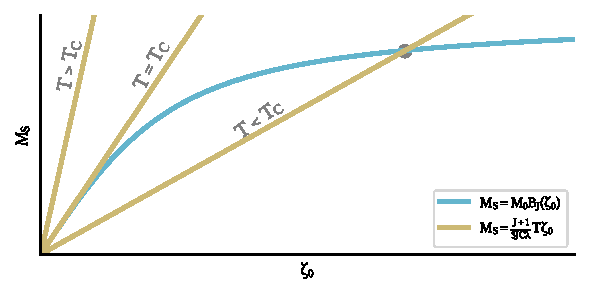
\includegraphics{figures/solgraph.pdf}
  \caption{\itshape Para $T<T\sub{C}$ aparece una magnetización espontanea
    $M\sub{S}$, resultado de la ecuación $M\sub{S} = f(M\sub{S})$.}
  \label{fig:solgraph}
\end{figure}

% Mon Apr  3 09:10:21 CEST 2017
Para $T=T\sub{C}$, la pendiente de ambas ecuaciones es la misma. Como
$\text{B}_J(ζ) ≃ \frac{J+1}{3J}ζ$ para $ζ≪1$, podemos reescribir las
ecuaciones recuadradas como
\begin{align}
  \frac{M\sub{S}}{M_0} &= \text{B}_J(ζ_0) = \frac{J+1}{3J}ζ_0 \\
  \frac{M\sub{S}}{M_0} &= \frac{J+1}{3JCλ} T ζ_0
\end{align}
igualamos los lados derechos para $T=T\sub{C}$, de forma que
\begin{equation}
  \begin{split}
    \frac{J+1}{3J}ζ_0 &=
    \frac{J+1}{3JCλ} T\sub{C}ζ_0 \\
    1 &= \frac{T\sub{C}}{Cλ} \\
    Cλ &= T\sub{C} \\
  \end{split}
\end{equation}

Normalmente, se conoce $T\sub{C}$ y se emplea esta ecuación para
averiguar $λ$. Por ejemplo, en el gadolinio
$T\sub{C}=\SI{292}{\kelvin}$ y
$C=μ_0Np^2\mb^2/3\kb=\SI{4.9}{\kelvin}$, por lo que $λ≃60$.

La susceptibilidad paramagnética ($T>T\sub{C}$) en el límite de $ζ$
pequeña se obtiene\footnote{Para obtenerla, hay que desarrolar en
  serie la función de Brillouin de la magnetización
  $M_0 \text{B}_J(ζ)$ y utilizar $χ = μ_0 M / B$.} como
\begin{equation}
  χ = \frac{C}{T-θ_p}
\end{equation}
donde $θ_p \equiv T\sub{C} = Cλ$, como se ha visto antes.
% Es un desarrollo en serie de la M(Brillouin) y dividir entre B
% Fix Rvs I prev graph

\subsection{Hamiltoniano de Heisenberg para campo medio}
El hamiltoniano de Heisenberg $\Ham = -2 \sum_{i>j} J_{ij}
\symbf{S}_i \symbf{S}_j$ se puede simplificar a una suma con una $J=f(λ)$
constante si se consideran sólo interacciones a primeros vecinos.
Para
cada espín $i$ se tiene una interacción con un campo local efectivo
$H^i = λng\mb S$:
\begin{equation}
  \Ham_i = - 2 \left( \sum_{j} J \symbf{S}_j \right) \symbf{S}_i ∼- μ_0
\end{equation}


\section{Teoría de Landau de transiciones de fase}
Se puede realizar un desarrollo similar al de los dieléctricos, pero
con las vaiables del ferromagnetismo: ahora el parámetro de orden es
$M$ en lugar de $P$.
Como se vio, al estar cerca de $T_C$ la energía libre
admite un desarrollo en serie:

\begin{equation}
  F\sub{L} (M,T,H) = -μ_0 H M + g_0 + \frac{1}{2} g_2 M^2 +
  \frac{1}{4} g_4 M^4 + \order{M^6}
  \label{eq:puraco}
\end{equation}
con $g_i = g_i(T)$.

Para $T<T\sub{C}$ el mínimo en $M=M\sub{S}$ implica que $g_2 < 0$ y
que $g_4>0$. Para $T>T\sub{C}$ el mínimo en $M=0$ indica $g_2, g_4 >
0$. Por lo tanto, $g_2$ debe cambiar de signo en $T\sub{C}$, por ello
definimos
\marginnote{
    Si no imponemos estas condiciones, no se obtienen $M=M\sub{S}$ y
    $M=0$. $g_2<0$ y $g_4>0$ hacen que salga un potencial de doble pozo
    con el pozo derecho más bajo, y $g_2, g_4>0$ hacen que salga un único
    pozo. Si $g_4<0$, los máximos se convierten en mínimos.
}
\begin{equation}
  g_2 = a(T-T\sub{C})
\end{equation}
donde $a > 0$ es una constante independiente de la temperatura.
Buscamos el mínimo de $F\sub{L}$:
\begin{equation}
  \pdv{F\sub{L}}{M} = 0 \ \rightarrow \ μ_0 H =  a (T-T\sub{C})M\sub{S} + g_4 M^3
\end{equation}

si $H→0$, $M=0$. Si no es así, simplificamos una $M\sub{S}$ y
resolvemos la ecuación de segundo grado ($H=0$):
\begin{equation}
  M = \sqrt{\frac{a}{g_4} (T\sub{C}-T)}
\end{equation}
Notar como hay dos mínimos.
Si la temperatura es muy cercana a $T\sub{C}$, se tiene $g_2 \propto
T-T\sub{C}  = 0$ y la resolución de \ref{eq:puraco} da la isoterma
crítica:
\begin{equation}
  M = \left( \frac{μ_0}{g_4} \right)^{\nicefrac{1}{3}} H^{\nicefrac{1}{3}}
\end{equation}
Existiendo un único mínimo.
En la vecindad de $T\sub{C}$,
\begin{equation}
  M^2 = \frac{μ_0}{g_4} \frac{H}{M} - \frac{2a}{g_4} (T-T\sub{C})
\end{equation}

ésta última ecuación es la base de los \emph{plots de Arrott-Belov}
(figura \ref{fig:abplot}),
empleados para hallar de forma precisa la temperatura de Curie. Se
dibujan varias isotermas $M(H)$ como $M^2, H/M$, y la única isoterma
que es extrapolable a $(0,0)$ es la crítica.

\begin{marginfigure}
  \centering
  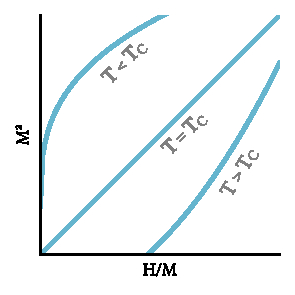
\includegraphics{figures/abplot.pdf}
  \caption{\itshape Plot de Arrott-Belov. La isoterma a $T\sub{C}$ es la única
    extrapolable al $(0,0)$.}
  \label{fig:abplot}
  \end{marginfigure}

% Errata en pdf que tienes, diapo que empieza por  For T<T_C a minimum

% Le molan los Arrot plot

% Tue Apr  4 07:45:48 CEST 2017
\section{Criterio de Stoner}
Hasta ahora, se ha establecido un paralelismo entre la teoría de
Brillouin de los ferroeléctricos y el fenómeno del ferromagnetismo
suponiendo electrones localizados, con la ayuda de la teoría de campo
molecular medio.

En los metales la hipótesis de electrones localizados no funciona, y
es necesario otro enfoque. Para ello, se establece un palalelismo con
el paramagnetismo de Pauli.

Vimos que el gas de electrones propicia una susceptibilidad $χ\sub{P}
= μ_0 \mb^2 D(E\sub{F})$ pequeña (paramagnetismo de Pauli).
En lugar del campo aplicado del paramagnetismo de Pauli, suponemos un
campo medio $\symbf{H}_i = λ \symbf{M} + \symbf{H}$ donde $λM ≫ H$
en un material ferromagnético.

\marginnote{
  \begin{flushright}
    \slshape
    ``El criterio de Stoner es un, es un criterio, que define una,
    define un parámetro, unas cantidades, lo decía mediante esto de
    aquí, que al multiplicarlo por el número de electrones en el nivel
    de Fermi, nos da idea de si el sistema está cerca de ser
    ferromagnético. En el Coey está con una letra griega un poco rara
    en vez de con una I.''
  \end{flushright}
  --- \textsc{Paulo Coelho}
}

En tres dimensiones, la densidad de estados es $D(E) ∝ \sqrt E$, y las
bandas de espin \textit{up} y \textit{down} se desplazan $ΔE = \mp μ_0 H
\mb$. La susceptibilidad generada es
\begin{equation}
  χ\sub{P} = \frac{μ_0M}{B} = \frac{μ(N_+ - N_- )}{B} = μ_0 \mb ^2 D(E\sub{F})
\end{equation}

Esta susceptibilidad es especialmente alta cuando la densidad de
estados en el nivel de Fermi $E\sub{F}$ es alta. Si es suficientemente
elevada, separar las bandas se vuelve energéticamente favorable y el
metal se vuelve de forma espontánea ferromagnético.

Asumamos, vista la teoría de campo molecular de Weiss, que el campo
interno $H^i$ es proporcional a $M$:
\begin{equation}
  H^i = λM + H
\end{equation}
La susceptibilidad de Pauli ante este $H^i$ será
\begin{equation}
  χ\sub{P} = M/H^i = \frac{M}{λM+H}
\end{equation}
Y por lo tanto, la susceptibilidad ante un campo externo $H$ será, sin
más que despejar el $H$ de la ecuación anterior,
\begin{equation}
  χ = \frac{M}{H} = \frac{χ\sub{P}}{1-λχ\sub{P}}
\end{equation}
Vemos que aumenta cuando $λχ\sub{P}<1$ y diverge cuando $λχ\sub{P}=1$.

Stoner expresó esta condición en términos de $D(E\sub{F})$. La energía
de canje su puede expresar como una función de la \emph{constante de
  Stoner}, $I = 2μ_0 λ \mb^2$:
\marginnote{Notar que se supone $H=0$.}
\begin{equation}
  - \frac{1}{2} μ_0 H^i M = - \frac{1}{2} μ_0 λ M^2 = -\frac{I}{4}
  \frac{(N_↑ - N_↓)^2}{N}
\end{equation}
empleando el número de átomos por unidad de volumen $N$ y la
magnetización $\mb (N_↑ - N_↓)$.

La divergencia se dará en metales con $λχ\sub{P}=1$. Introduciendo la
constante $N=D(E\sub{F})/2N$, se obtiene
\begin{equation}
  \boxed{
    I N(E\sub{F}) ≥ 1
  }
\end{equation}
expresión conocida como \emph{criterio de Stoner}. Los metales que lo
cumplen (hierro, cobalto, y níquel) tienen una constante de
intercambio $I$ del orden del ancho de la banda de energía y son
ferromagnéticos.

% Wed Apr  5 09:04:33 CEST 2017

\marginnote{
  \begin{flushright}
    \slshape
    ``Odio los espines.''
  \end{flushright}
  --- \textsc{A student}
}

% </endday>

% Tue Apr 18 08:05:20 CEST 2017
\section{Spin waves}

Las \textit{spin waves} son excitaciones de baja energía ($E∼\kb T$) en materiales
ferromagnéticos a bajas temperaturas. Las frecuencias involucradas están en el rango
del infrarojo y las microondas.

Para obtener la relación de dispersión para las cuasipartículas
responsables, los \emph{magnones}, se empleará una descripción
semiclásica. A continuación, se cuantizará su energía y se
interpretará dicha cuantización en términos de cambios de espín
\textit{up} a espín \textit{down}.


El estado fundamental de un material unidimensional ferromagnético con
$N$ espines $S_p$
paralelos puede describirse con un hamiltoniano de Heisenberg a
primeros vecinos:
\marginnote{$↑_1 ↓_2 ↑_3 ↑_4 ↑_5 ⋯ ↑_p ⋯ ↑_{N-1} ↓_N$}
\begin{equation}
  U = -2J \sum_{p=1}^N \symbf{S}_p \symbf{S}_{p+1}
\end{equation}

con $J$ la integral de canje y $ℏ \symbf{S}_p$ el momento angular de
un espín en la posición $p$. Suponiendo que los $\symbf{S}$ son
vectores clásicos, en el estado fundamental $\symbf{S}_p
\symbf{S}_{p+1} = S^2$ y la energía de canje resulta $U_0 = - 2NJS^2$.

Puede considerarse que la excitación de energía más baja corresponde
al \textit{flip} de un sólo espín. En tal caso, empleando el
hamiltoniano recién escrito vemos un aumento en la energía de $8JS^2$ unidades\footnotemark.
\footnotetext{
  El \textit{flip} de un espín $p$ afecta a los sumandos $-2J
  \symbf{S}_p \symbf{S}_{p+1}$ y $-2J \symbf{S}_{p-1}
  \symbf{S}_p$. Ambos valían $-2JS^2$ y ahora valen $+2JS^2$, luego
  $ΔU = 2JS^2 - (-2JS^2) = 4JS^2$ por cada sumando, $8JS^2$ teniendo
  en cuenta los dos.
}
Como $\kb T\sub{C}= \frac{2}{3}JZS(S+1) ∼ J$, la situación es cara
energéticamente. \emph{Excitaciones de menor energía pueden lograrse si se
permite que todos los espines compartan la inversión.}

Escribamos los términos del hamiltoniano involucrados en una inversión
local como la descrita anteriormente:
\begin{equation}
  \begin{split}
    \Ham_p &= [-2J \symbf{S}_p \symbf{S}_{p+1}] +
    [-2J \symbf{S}_{p-1} \symbf{S}_{p}] \\
    &=
    -2J \symbf{S}_p(\symbf{S}_{p-1}+\symbf{S}_{p+1}) = - \symbf{μ}_p
    \underbrace{\left( - \frac{2J}{g\mb} [ \symbf{S}_{p-1}+
        \symbf{S}_{p+1}] \right)}_{\symbf{B}_p} = -\symbf{μ}_p
    \symbf{B}_p
  \end{split}
\end{equation}
donde $\symbf{B}_p$ es un campo molecular promedio, igual para todos
los espines y se ha empleado $\symbf{μ}_p = -g\mb \symbf{S}_p$.
La ecuación del movimiento del momento magnético $ℏ
\symbf{S}_p$ viene regida por el momento $\symbf{μ}_p × \symbf{B}_p$:
\begin{equation}
    ℏ \dv{\symbf{S}_p}{t} = \symbf{μ}_p × \symbf{B}_p
    = - \frac{g\mb}{ℏ} \symbf{S}_p × \symbf{B}_p =
    \frac{2J}{ℏ}(\symbf{S}_p×\symbf{S}_{p-1} \ + \ \symbf{S}_p × \symbf{S}_{p+1})
\end{equation}

Suponiendo una excitación de amplitud pequeña ($S_p^x,S_p^y ≪ S ≃
S_p^z$), podemos escribir los componentes de ecuación anterior como
\begin{marginfigure}
  \centering
  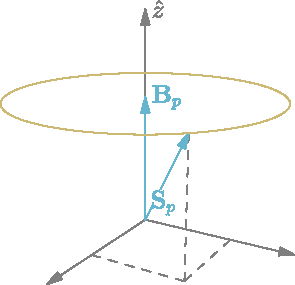
\includegraphics{figures/spin.pdf}
  \caption{\itshape Componentes del espín $\symbf{S}_p$, que gira ante el
    campo promedio $\symbf{B}_p$.}
  \label{fig:spin}
\end{marginfigure}
\begin{equation}
  \begin{split}
    \dot{S_p^x} &= \frac{2JS}{ℏ} (2S_p^y - S_{p-1}^y - S_{p+1}^y) \\
    \dot{S_p^y} &= -\frac{2JS}{ℏ} (2S_p^x - S_{p-1}^x - S_{p+1}^x) \\
    \dot{S_p^z} &= 0
  \end{split}
  \label{eq:systemloco}
\end{equation}

En analogía con los fonones, suponemos una solución estacionaria
$\symbf{S}_p = (u\hat{x} + v\hat{y}) e^{i(pka - ωt)}$ con $u,v ∈
\mathbb{R}$, $p ∈ \symbf{Z}$ y $a$ la constante de red. Al sustituir
en el sistema de ecuaciones \eqref{eq:systemloco} obtenemos
\begin{equation}
  \begin{split}
    -i ω u = \frac{2JS}{ℏ} (2- e^{-ika} - e^{ika})v &= \frac{4JS}{ℏ}
    (1-\cos ka) v \\
    -i ω v = -\frac{2JS}{ℏ} (2- e^{-ika} - e^{ika})u &= -\frac{4JS}{ℏ}
    (1-\cos ka) u \\
  \end{split}
\end{equation}
sistema de ecuaciones resoluble si el determinante de sus coeficientes
es nulo:
\begin{equation}
  \mqty| iω && \frac{4JS}{ℏ}(1-\cos ka) \\
  -\frac{4JS}{ℏ}(1-\cos ka) && iω | = 0
\end{equation}
de forma que obtenemos (figura \ref{fig:magnon})
\begin{equation}
  \boxed{ℏω(k) =4JS(1-\cos ka)}
\end{equation}
y $v=-iu$, correspondiendo a una precesión alrededor de $\symbf{B}_p
≃ \hat{z}$. Para longitudes de onda $λ=2π/k$ largas podemos aproximar
$ka≪1$ y $\cos ka ≃ \oh (k a)^2$, por lo que
\begin{equation}
  ℏω(k)≃ 2JSa^2 \ k^2
\end{equation}
\begin{marginfigure}[+1cm]
  \centering
  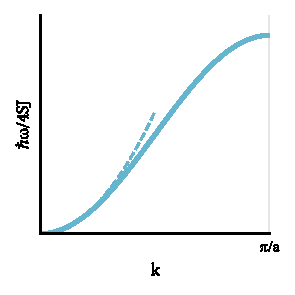
\includegraphics{figures/magnon.pdf}
  \caption{\itshape Relación de dispersión para las \textit{spin waves}. Cerca
    del origen es proporcional a $k^2$.}
  \label{fig:magnon}
\end{marginfigure}
despreciando el término constante.

Mientras para los fonones se tenía a baja $k$ que $ω ∼ k$, aquí se
obtiene $ω∼k^2$. Si suponemos un cristal cúbico tridimensional con interacciones a
primeros vecinos, la relación de dispersión se escribe como
\begin{equation}
  ℏω =2JS \left( z - \sum_{δ} \cos \symbf{k}\symbf{δ} \right)
\end{equation}
donde la suma es sobre los vectores $z$ denotados por $\symbf{δ}$ que
conectan al átomo central con sus primeros vecinos\footnote{Notar que
  la onda sólo se propaga en una dirección, que aquí se ha supuesto
  $\hat{z}$.}. Aproximando a ondas largas ($ka≪1$) se obtiene:
\begin{equation}
  ℏω =2JSa^2\ k^2 = D_{sω} k^2
  \label{eq:thisispainful}
\end{equation}
donde $D_{sω}$ es la constante de \emph{magnetic stiffness}, con
valores cercanos al \SI{}{\eV}, y $a$ es la constante de red.
\marginnote{
  \begin{center}
      \begin{tabular}{lc}
        \toprule
        Material & $D_{sω}(T=\SI{295}{\kelvin})$ \\
        \midrule
        Fe & \SI{281}{\milli\eV\angstrom\squared} \\
        Co & \SI{500}{\milli\eV\angstrom\squared} \\
        Ni & \SI{364}{\milli\eV\angstrom\squared} \\
        \bottomrule
      \end{tabular}
  \end{center}
}

La cuantización de las \textit{spin waves} es análoga a la de los
fonones o los fotones; la energía de un modo de frecuencia $ω_k$ con
$n_k$ \emph{magnones} es $E_k = (n_k + \oh) ℏω_k$. La excitación de un
magnón corresponde a la inversión de un espín $\oh$.


\marginnote{
  Otra forma de llegar a la relación de dispersión es entrar en segunda
  cuantización y emplear operadores de creación y destrucción
  $S_+,S_-$. El libro de Ashcroft tiene más detalles al respecto.
}

\subsection{Excitaciones térmicas de magnones}
\marginnote{El calor específico va como $T^2$ para fonones,
  $T^{\nicefrac{3}{2}}$ para magnones y como $T$ para electrones.}
El concepto de \textit{spin waves} es muy útil para explicar la
dependencia térmica de la magnetización en el rango de bajas
temperaturas. En equilibrio térmico, el número promedio de magnones excitados
en el modo $k$ viene dado por una distribución de Plank\footnote[][+1cm]{Es un
  caso especial de la distribución de Bose-Einstein, con $E→ℏω$.}:
\begin{equation}
  \expval{n_k} = \frac{1}{e^{β ℏω} - 1}
\end{equation}
A una temperatura $T$, podemos hallar el número total de magnones como
$ \sum_{k} n_k = \int D(ω) \expval{n(ω)} \dd{ω}$, donde $D(ω)$ es el número
de modos de magnon por rango unitario de frecuencia. La integral te
toma sobre los $\symbf{k}$ permitidos, que son los que delimitan la
primera zona de Brillouin.

A temperaturas suficientemente bajas, podemos evaluar la integral en
$ω∈[0,∞)$, ya que $n$ cae exponencialmente conforme aumentamos $ω$.
\marginnote{Los magnones tienen una sola polarización por
cada $\symbf{k}$.}
Tenemos en cuenta que en 3D el número de modos de un vector de onda
menores que $k$ es\footnote{Hay $\nicefrac{4}{3}πk^2 \dd{k}$ estados
  entre las k-esferas, dividido entre $(2π)^3$ estados totales.} $(2π)^{-3} \frac{4}{3} π k^3$, y
escribimos el número de magnones $D(ω)\dd{ω}$ con frecuencia $ω$
dentro de un $\dd{ω}$ como
\begin{equation}
  D(ω) \dd{ω} = \left( \frac{1}{2π} \right)^3 (4πk^2) \dv{k}{ω} \dd{ω}
\end{equation}
En la aproximación de onda larga ($ka≪1$) tenemos
\begin{equation}
\dv{ω}{k} =
\frac{4JSa^2}{ℏ}k = 2 (4JSa^2 / ℏ)^\oh \ (ω)^\oh
\end{equation}
empleando la ecuación \eqref{eq:thisispainful}. Sustituyendo en el
resultado anterior para $D(ω) \dd{ω}$, se obtiene
\begin{equation}
  D(ω) = \frac{1}{4π^2} \left( \frac{ℏ}{4JSa^2} \right)^{3/2} ω^{1/2}
\end{equation}

Ahora que se conoce $D(ω)$ (y $\expval{n_k}$ por la ley de plank), se
puede realizar la integral de $\sum_k n_k$, obteniendo
\marginnote{$\int_0^∞ \frac{\sqrt{x}}{e^{x}-1} \dd{x} =
  \frac{\sqrt{π}}{2} ζ(\nicefrac{3}{2}) ≃ 4π^2 ⋅ 0.0586$}
\begin{equation}
  \sum_{k} n_k = \int D(ω) \expval{n(ω)} \dd{ω} = ⋯ = 0.0587 \left(
    \frac{\kb T}{2JSa^2} \right)^{3/2}
\end{equation}

El número de átomos por unidad de volumen es $Q/a^3$, donde $Q$
depende de la red\footnotemark.
\footnotetext{
  \begin{flushleft}
    \begin{tabular}{cc}
      \toprule
      Red & Q \\
      \midrule
      SC & 1 \\
      BCC & 2\\
      FCC & 4\\
      \bottomrule
    \end{tabular}
  \end{flushleft}
}
Con él, calculamos el cambio $ΔM = M-M(0)$ de la magnetización:
\begin{equation}
  \boxed{
  \frac{ΔM}{M(0)} = \frac{\sum_{k}n_k}{NS} = \frac{0.0587}{SQ} \left(
    \frac{\kb T}{2JS} \right)^{3/2} ∝ T^{2/3}
  }
\end{equation}
relación conocida como \emph{ley de Bloch}, y confirmada
experimentalmente hasta $T\sub{C}$ e incluso superiores.

% \section{Dispersión magnética de nutrones}

% Wed Apr 19 09:30:15 CEST 2017
% </spinwaves>


% Hablemos sobre el scattering inelástico de neutrones. Mientras el
% elástico da idea de la distribución periódica de μ's, el inelástico
% aporta información sobre las excitaciones de la red y los intercambios
% de energía.

% Tue Apr 25 08:04:09 CEST 2017

\chapter{Interacciones ferromagnéticas}

El canje que hemos estado comentando hasta ahora es canje
directo\footnote{AKA \textit{Diret exchange}.}. Los átomos están
bastante próximos como para que los electrones puedan interactuar
directamente.

En otras situaciones (por ejemplo, óxidos) las nubes de carga
electrónica están separadas entre ellas. La interacción de canje
(supercanje) se da a traves de los átomos intermedios. En el caso del
canje indirecto, la interacción se transmite a traves de dipolos entre
las nubes de carga.

\section{Interacciones magnéticas en metales}

\subsection{Canje directo}
La aproximación más sencilla es la de canje directo, junto a una
aproximación de \textit{tight-binding}\footnote{Los electrones están
  prácticamente localizados en el átomo}. Esta última se traduce en
\begin{equation}
  \Ham = \sum_{ij} t_{ij} c_i^\dagger c_j
\end{equation}
donde los operadores escalera $c$ crean electrones y $t_{ij}$ es la
\textit{transfer integral}. Si la suma es a primeros vecinos, $t_{ij}
= i, \ ∀ i,j$. La anchura $W$ de la banda en este modelo es $W=2tZ ∼
\SI{1}{\eV}$, donde $Z$ es el número de primeros vecinos.

Según la ocupación de los niveles, puede predecirse si la interacción
será antiferromagnética o ferromagnética:
\begin{itemize}
\item Cuando la banda está cerca de estar medio llena la interacción
  es antiferromagnética, ya que sólo es energéticamente favorable que
  el espín se expanda hacia la banda vecina si están alineadas de
  forma antiparalela:
  \begin{center}
    \orbital{\textcolor{NiceRed}{↓}}\orbitalsep\orbital{\textcolor{NiceRed}{↓}}\orbitalsep\orbital{\textcolor{NiceRed}{↓}}
    \orbital{↑}\orbitalsep\orbital{↑}\orbitalsep\orbital{↑} →
    \orbital{\textcolor{NiceRed}{↓}}\orbitalsep\orbital{\textcolor{NiceRed}{↓}}\orbitalsep\orbital{\textcolor{NiceRed}{ }}
    \orbital{↑\textcolor{NiceRed}{↓}}\orbitalsep\orbital{↑}\orbitalsep\orbital{↑}
  \end{center}
\item Las bandas casi vacías o casi llenas suelen tener interacciones
  ferromagnéticas, ya que los espines pueden saltar en estados vacíos
  aún estando las bandas alineadas de forma paralela:
  \begin{center}
    \orbital{\textcolor{NiceRed}{↑}}\orbitalsep\orbital{\textcolor{NiceRed}{↑}}\orbitalsep\orbital{\textcolor{NiceRed}{   }}
    \orbital{↑}\orbitalsep\orbital{↑ }\orbitalsep\orbital{ } →
    \orbital{\textcolor{NiceRed}{↑}}\orbitalsep\orbital{ }\orbitalsep\orbital{\textcolor{NiceRed}{ }}
    \orbital{↑}\orbitalsep\orbital{↑}\orbitalsep\orbital{\textcolor{NiceRed}{↑}}
  \end{center}
  \begin{center}
    \orbital{\textcolor{NiceRed}{↑↓}}\orbitalsep\orbital{\textcolor{NiceRed}{↑↓}}\orbitalsep\orbital{\textcolor{NiceRed}{↑  }}
    \orbital{↑↓}\orbitalsep\orbital{↑↓}\orbitalsep\orbital{↑} →
    \orbital{\textcolor{NiceRed}{↑ }}\orbitalsep\orbital{\textcolor{NiceRed}{↑↓}}\orbitalsep\orbital{\textcolor{NiceRed}{↑}}
    \orbital{↑↓}\orbitalsep\orbital{↑↓}\orbitalsep\orbital{↑\textcolor{NiceRed}{↓}}
  \end{center}
\end{itemize}
% Coey 4 win

Conforme aumentamos $t$, los electrones se deslocalizan (saltan)
independientemente de su espín. Por encima del escandio, los
materiales ya no son ferromagnéticos por su alta $t$.

% Wed Apr 26 09:22:17 CEST 2017
\subsection{Canje indirecto}
Si los momentos localizados están muy separados, no interaccionan de
forma directa. Es necesario un intermediario, como muestra el
hamiltoniano de Zener:
\begin{equation}
  \Ham_s = - J_{Sd} Ω \abs{Ψ}^2 \symbf{S} \symbf{s}
\end{equation}
con $Ω$ el volumen del orbital \textit{d}, $\abs{Ψ}$ la función de
ondas de los electrones \textit{s} y $J_{Sd}∼ \SI{}{\eV}$.
Este modelo (llamado a veces \textit{modelo s-d}) se intentó aplicar
en las tierras raras, cuyo momento del orbital 4f está muy localizado.
En él, los electrones $\symbf{s}$ de la capa conducción interaccionan
con otros $\symbf{s}$ mediante los electrones $\symbf{S}$ de otras
capas. Se asume que la banda receptora posee una polarización
uniforme, bien paralela o antiparalela a los espines nucleares.

Otro modelo (\textit{interacción RKKY}) propone un
\begin{equation}
  J_\mathit{eff} = \frac{9πJ_{sf}^2v^2}{64ε\sub{F}} F(ζ)
\end{equation}
con $F(ζ)=(\sin ζ - ζ \cos ζ)/ζ^4$ fuertemente oscilante (figura
\ref{fig:RKKY}) y $ζ=2k\sub{F}r$.
\begin{marginfigure}[-3cm]
  \centering
  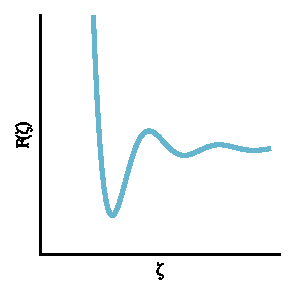
\includegraphics{figures/RKKY.pdf}
  \caption{\itshape Las oscilaciones RKKY se apagan para $ζ→∞$,
    quedando $F(ζ)→0$. En el origen, divergen.}
  \label{fig:RKKY}
\end{marginfigure}

En él un único espín crea una perturbación de espín oscilante e inhomogénea
que decae como $r^{-3}$.


%Dzyaloshinski-Moriya not in exam.

\section{Interacciones magnéticas en aislantes}
Los aislantes están caracterizados por tener electrones localizados.
Los ejemplos más representativos son los óxidos metálicos.

\subsection{Supercanje}
\marginnote{\textcolor{gray}{Go, Jhonny go, go, go, Jhonny B. Goodenough!}}

La interacción más frecuente en óxidos de metales \textit{3d} es el
\emph{supercanje}. En estos compuestos existen átomos de oxígeno entre
los del metal, lo que causa un solapamiento muy pequeño entre los
\textit{3d} del metal. El supercanje se produce a través de la
hibridación de los orbitales \textit{3d} del metal con los \textit{2d}
del oxígeno; la interacción $J$ implica la transferencia virtual de dos
electrones, con la formación instantánea de un estado excitado de
carga positiva.

La ocupación y degeneración de los orbitales \textit{3d} son críticos
para determinal el signo e intensidad de la $J$ del supercanje.
Goodenough y Kanamori establecieron una serie de reglas para
determinar $J$, que fueron reformuladas por P.\,W.\,Anderson de la
siguiente forma:
\begin{itemize}
\item Cuando dos cationes presentan lóbulos \textit{3d} monoocupados,
  uno apuntando hacia el otro, se tiene un solapamiento grande, con
  canje intenso y de tipo antiferromagnético ($J<0$). Es el caso más
  habitual para enlaces M--O--M con orientaciones entre
  \SI{120}{\degree} y \SI{180}{\degree}.
\item Cuando los dos cationes presentan una integral de solapamiento
  entre estados monoocupados nula por simetría el canje el
  ferromagnético y relativamente débil. Esta situación se da para
  enlaces M--O--M que forman ángulos de \SI{90}{\degree}.
\item Cuando los dos cationes se solapan entre un estado \textit{3d}
  monoocupado y un estado del mismo tipo doblemente ocupado o vacío,
  el canje es también ferromagnético y relativamente débil.
\end{itemize}

\subsection{Doble canje}
Se da entre algunos iones que se encuentran en distintos estados de
oxidación, un caso típico es la perovskita cúbica. En lo que sigue,
consideremos la estructura La\textsubscript{1-x}Ca\textsubscript{x}
MnO\textsubscript{3} (figura \ref{fig:hateibarra}).

\begin{marginfigure}
  \centering
  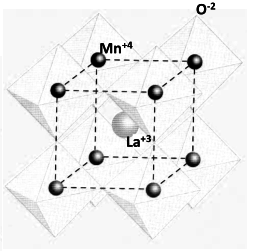
\includegraphics[width=0.8\textwidth]{figures/lacamno.png}
  \caption{\itshape Estructura del cristal de
    La\textsubscript{1-x}Ca\textsubscript{x}MnO\textsubscript{3}.}
  \label{fig:hateibarra}
\end{marginfigure}

\marginnote{Muy de entrar en el examen:
  \begin{flushright}
    \emph{``
      En el supercanje se forman funciones de onda ligadas a
      hibridaciones con el oxígeno (Goodenough) o electrones a secas
      (Anderson). En el doble canje hay distintos estados iónicos
      (Mn\textsuperscript{+3}, Mn\textsuperscript{+4}), y el oxígeno hace de
      puente por el que pueden pasar dichos electrones.''}
  \end{flushright}
}

En algunas celdas, el ion central es el La\textsuperscript{3+}, pero
en otras es el Ca\textsuperscript{2+}. Esto ocasiona cambios en el
número de oxidación de los átomos de manganeso que lo rodean y en el
campo eléctrico del cristal, que posee menor simetría en el caso del
Mn\textsuperscript{3+}.

Veamos detenidamente el proceso de doble canje, siguiendo a los dos
electrones (\textcolor{NiceRed}{↑}\textcolor{NiceBlue}{↑})
involucrados:

\begin{enumerate}
\item Al principio, tenemos un electrón de más en el manganeso de la
  izquierda. El orbital \textit{p} del oxígeno, en medio, esta lleno.
  El manganeso interactuará con el oxígeno con su orbital $e_g$.

\begin{center}
  \begin{tikzpicture}
    \draw (0,0) -- (2,0);
    \draw (0,-0.5) -- (2,-0.5) node[near start] {\textcolor{NiceRed}{↑}};
    \node[right] at (2,-0.25) {$e_g$};

    \draw (0,-1.5) -- (2,-1.5) node [near end] {↑};
    \draw (0,-2.0) -- (2,-2.0) node [midway] {↑};
    \draw (0,-2.5) -- (2,-2.5) node [near start] {↑};
    \node[right] at (2,-2.0) {$t_{2g}$};

    \node[below] at (1,-2.5) {Mn\textsuperscript{3+}};
  \end{tikzpicture}
  \quad
  \raisebox{1.5cm}{
    \begin{tikzpicture}
      \draw (0,0) to[out=-30, in=-90] (1,0) to[out=90, in=30] (0,0);
      \draw (0,0) to[out=-150, in=-90] (-1,0) to[out=90, in=150] (0,0);
      \node at (0,0) {\textcolor{NiceBlue}{↑}↓};
    \end{tikzpicture}
  }
  \quad
  \begin{tikzpicture}
    \draw (0,0) -- (2,0);
    \draw (0,-0.5) -- (2,-0.5);
    \node[right] at (2,-0.25) {$e_g$};

    \draw (0,-1.5) -- (2,-1.5) node [near end] {↑};
    \draw (0,-2.0) -- (2,-2.0) node [midway] {↑};
    \draw (0,-2.5) -- (2,-2.5) node [near start] {↑};
    \node[right] at (2,-2.0) {$t_{2g}$};

    \node[below] at (1,-2.5) {Mn\textsuperscript{4+}};
  \end{tikzpicture}
\end{center}

\item Un electrón del oxígeno pasa \emph{con la misma orientación} al
  Mn\textsuperscript{4+}, transformándolo en Mn\textsuperscript{3+}.

\begin{center}
  \begin{tikzpicture}
    \draw (0,0) -- (2,0);
    \draw (0,-0.5) -- (2,-0.5) node[near start] {\textcolor{NiceRed}{↑}};
    \node[right] at (2,-0.25) {$e_g$};

    \draw (0,-1.5) -- (2,-1.5) node [near end] {↑};
    \draw (0,-2.0) -- (2,-2.0) node [midway] {↑};
    \draw (0,-2.5) -- (2,-2.5) node [near start] {↑};
    \node[right] at (2,-2.0) {$t_{2g}$};

    \node[below] at (1,-2.5) {Mn\textsuperscript{3+}};
  \end{tikzpicture}
  \quad
  \raisebox{1.5cm}{
    \begin{tikzpicture}
      \draw (0,0) to[out=-30, in=-90] (1,0) to[out=90, in=30] (0,0);
      \draw (0,0) to[out=-150, in=-90] (-1,0) to[out=90, in=150] (0,0);
      \node at (0,0) {↓};
    \end{tikzpicture}
  }
  \quad
  \begin{tikzpicture}
    \draw (0,0) -- (2,0);
    \draw (0,-0.5) -- (2,-0.5) node[near start] {\textcolor{NiceBlue}{↑}};
    \node[right] at (2,-0.25) {$e_g$};

    \draw (0,-1.5) -- (2,-1.5) node [near end] {↑};
    \draw (0,-2.0) -- (2,-2.0) node [midway] {↑};
    \draw (0,-2.5) -- (2,-2.5) node [near start] {↑};
    \node[right] at (2,-2.0) {$t_{2g}$};
    \node[below] at (1,-2.5) {Mn\textsuperscript{3+}};
  \end{tikzpicture}
\end{center}

\item Aprovechando el hueco, el electrón del Mn\textsuperscript{3+}
  original pasa al orbital del oxígeno. El ion es ahora Mn\textsuperscript{4+}.

\begin{center}
  \begin{tikzpicture}
    \draw (0,0) -- (2,0);
    \draw (0,-0.5) -- (2,-0.5);
    \node[right] at (2,-0.25) {$e_g$};

    \draw (0,-1.5) -- (2,-1.5) node [near end] {↑};
    \draw (0,-2.0) -- (2,-2.0) node [midway] {↑};
    \draw (0,-2.5) -- (2,-2.5) node [near start] {↑};
    \node[right] at (2,-2.0) {$t_{2g}$};

    \node[below] at (1,-2.5) {Mn\textsuperscript{4+}};
  \end{tikzpicture}
  \quad
  \raisebox{1.5cm}{
    \begin{tikzpicture}
      \draw (0,0) to[out=-30, in=-90] (1,0) to[out=90, in=30] (0,0);
      \draw (0,0) to[out=-150, in=-90] (-1,0) to[out=90, in=150] (0,0);
      \node at (0,0) {\textcolor{NiceRed}{↑}↓};
    \end{tikzpicture}
  }
  \quad
  \begin{tikzpicture}
    \draw (0,0) -- (2,0);
    \draw (0,-0.5) -- (2,-0.5) node[near start] {\textcolor{NiceBlue}{↑}};
    \node[right] at (2,-0.25) {$e_g$};

    \draw (0,-1.5) -- (2,-1.5) node [near end] {↑};
    \draw (0,-2.0) -- (2,-2.0) node [midway] {↑};
    \draw (0,-2.5) -- (2,-2.5) node [near start] {↑};
    \node[right] at (2,-2.0) {$t_{2g}$};
    \node[below] at (1,-2.5) {Mn\textsuperscript{3+}};
  \end{tikzpicture}
\end{center}

\end{enumerate}

Ha habido un movimiento neto de un electrón de un ion al otro, que se
ve facilitado si no cambia su espín en el proceso. Si bien el proceso
puede parecerse superficialmente al supercanje, hay que notar que aquí
es necesario que una de las especies tenga un electrón de más.

Los electrones de la capa $t_{2g}$ inferior dotan al sistema de
momentos magnéticos, mientras que el electrón en $e_g$ que salta de un
ion a otro va ordenando los momentos magnéticos y alineándolos.
Además, hace que el estado doblete sea inestable y causa distorsiones
locales en la red, que causan el ya visto efecto Jahn-Teller. La
interacción $J$ es completamente indirecta, sin solapamiento en las
distribuciones de carga de los iones magnéticos, de tipo
ferromagnético, e intensa. La integral de transferencia es
\begin{equation}
  t = t_0 \cos \nicefrac{Θ}{2}
\end{equation}
con $Θ$ la desviación angular respecto a \SI{180}{\degree} causada por
los cambios en el estado iónico; la red está deformada (figura
\ref{fig:deformed}). Cuanto más deformación existe, mayor es la
interacción ferromagnética.

\begin{marginfigure}
  \centering
  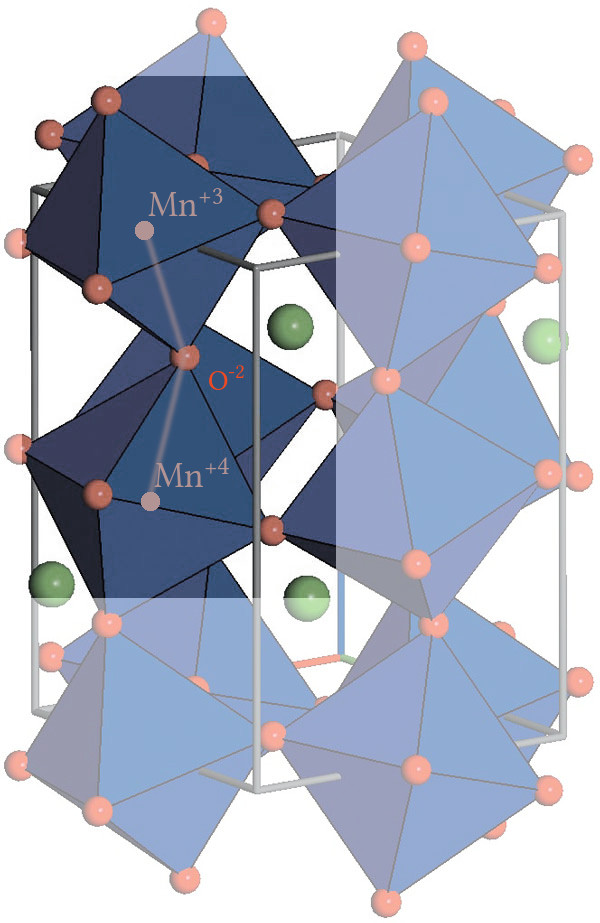
\includegraphics[width=0.8\textwidth]{figures/deformed.jpg}
  \caption{\itshape La estructura de la perovskita está deformada, lo que hace
    que el ángulo Mn--O--Mn no sea de \SI{180}{\degree}.}
  \label{fig:deformed}
\end{marginfigure}

La interacción de doble canje permite explicar el fenómeno de la
\emph{magnetoresistencia colosal}, en el cual un material puede variar
su resistencia \emph{ordenes de magnitud} al variar el campo magnético
aplicado, en lugar de un 5\% típico en la magnetoresistencia típica.
En la fase paramagnética ($T>T\sub{C}$) el material se comporta como
un aislante y aumenta su resistencia al disminuir la temperatura,
hasta alcanzar súbitamente su $ρ$ máxima. Si se disminuye más la
temperatura, se produce un ordenamiento magnético del material y pasa
a ser un conductor ferromagnético, bajando de forma muy marcada su
resistividad. El efecto es mucho menos marcado para campos externos
altos, siendo $ρ$ más baja y fluctuando menos.

Los electrones itinerantes de una red cristalina pueden verse
localizados por fenómenos de desorden (no considerados aquí) o bien
por distorsiones locales como las vistas anteriormente. Las
distorsiones locales dan lugar a $\cancel{\text{catedráticos}}$ pozos
de potencial llamados \emph{polarones} que hacen tender a los
electrones a permanecer en determinados puntos del material.

% Skipping antiferro.
\section{Antiferromagnetismo y ferrimagnetismo}
Un ejemplo clásico de material antiferromagnético es el MnO, de
estructura FCC. Un análisis de scattering de netrones a menos de
\SI{80}{\kelvin} da un parámetro de red de \SI{8.85}{\angstrom},
mientras que si se realiza con rayos X se obtienen
\SI{4.43}{\angstrom}. Esto permite concluir la ordenación
cristalográfica (química) tiene un parámetro de red de
\SI{4.5}{\angstrom}, pero a temperaturas bajas los momentos magnéticos
se ordenan en planos (111) de espín \textit{up} y espín \textit{down},
de forma que se obtiene una celda unidad magnética el doble de grande
(figura \ref{fig:mno}). Esto se manifiesta como unos picos extra en la
difracción de neutrones para temperaturas bajas.

\begin{marginfigure}
  \centering
  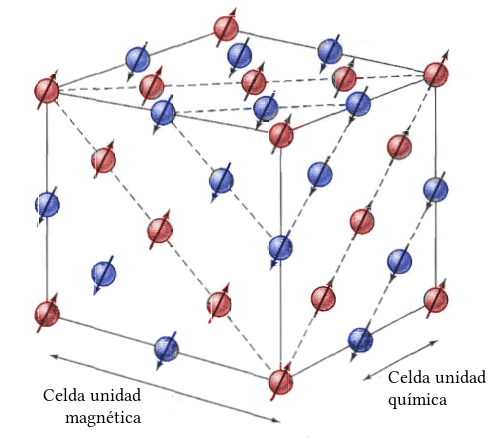
\includegraphics[width=0.8\textwidth]{figures/mno.png}
  \caption{\itshape La celda unidad magnética del MnO es el doble de
    grande que la celda química. Se muestran los espines
    \textcolor{BrickRed}{up} y \textcolor{NavyBlue}{down}.}
  \label{fig:mno}
\end{marginfigure}

Los materiales antiferromagnéticos ordenan sus espines de forma
antiparalela con momento neto cero a temperaturas por debajo de la
\emph{temperatura de Neel}, $T\sub{N}$. Su susceptibilidad no diverge
en ella, sino que tiene un pequeño pico, como muestra la figura \ref{fig:susccompare}.

\begin{figure}
  \centering
  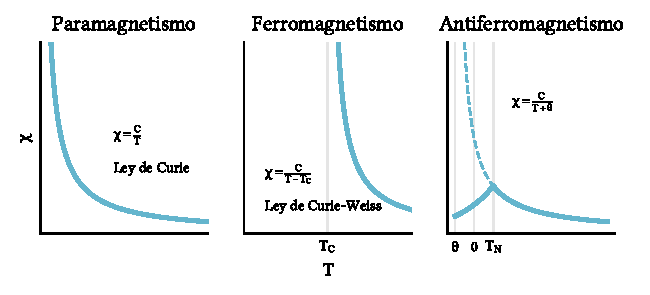
\includegraphics{figures/susccompare.pdf}
  \caption{ \itshape La susceptibilidad magnética es siempre la
    paramagnética por encima de las temperaturas críticas $T\sub{N}$y
    $T\sub{C}$, con comportamientos diferentes por debajo.}
  \label{fig:susccompare}
\end{figure}

Los materiales ferrimagnéticos, como la magnetita Fe\textsubscript{3}
O\textsubscript{4}, pueden modelarse como materiales
antiferromagnéticos con dos subredes distintas. La magnetización de
saturación a $T=\SI{0}{\kelvin}$ no corresponde a la alineación
paralela de los momentos magnéticos de los iones paramagnéticos;
analicemos el caso de la magnetita.

En su estructura cristalina, los iones Fe\textsuperscript{3+} se
encuentran en un estado con espín $\nicefrac{5}{2}$ y momento orbital
nulo. Cada uno de ellos debería contribuir con $5\mb$ al momento
magnético de saturación. Por otra parte, los Fe\textsuperscript{2+}
tienen espín $2$ y deberían contribuir con $4\mb$. Dado que cada
molécula de magnetita tiene 2 iones Fe\textsuperscript{3+} y un
Fe\textsuperscript{2+}, deberíamos tener $(2×5 + 4)\mb = 14\mb$ si
todos los espines estuvieran paralelos.

El valor expermental es $4.1\mb$, consistente con que los iones
Fe\textsuperscript{3+} se ordenen de forma antiparalela y los
Fe\textsuperscript{2+} de forma paralela, obteniéndose
$5\mb+(-5)\mb+4\mb = 4\mb$. Experimentos de difracción de neutrones
confirman esta teoría.

% Tue May  9 09:15:43 CEST 2017


\section{Dominios ferromagnéticos}
\marginnote{Es tentador (o a mí me lo pareció) pensar que los espines
deberían tender a alinearse entre todos, y la energía debería ser
mínima para un solo dominio magnético, no para muchos antiparalelos.
No obstante, si todos los espines están alineados, la energía dipolar
magnética es brutal. ↑↑↑↑ son 4 polos norte pegados y 4 polos sur
pegados, eso no es estable. ↑↓↑↓ sí lo es. Esta energía quiere crear
↑↓↑↓, la de canje quiere ↑↑↑↑, y compiten.}

En ausencia de campo magnético, los materiales ferromagnéticos se
dividen en dominios magnéticos de imanación local no nula e imanación
global nula. Es necesario un campo magnético para crear una imanación
global neta.

Si bien al principio su observación experimental dependía de
suspensiones de coloides magnéticos sobre placas de materiales
ferromagnéticos\footnote{Recordar que $\symbf{F}∝∇\symbf{B}$, no
  $\symbf{F}∝\symbf{B}$, lo que hace que las partículas se acumulen
  en los bordes de los dominios en lugar de en los dominios.},
actualmente el uso de microscopía de fuerza atómica con
\textit{cantilever} magnético es el método frecuente.

La \emph{microscopía de Lorentz} es otra forma de observar
experimentalmente los dominios. Consiste en utilizar microscopía
electrónica de transmisión y observar la deflexión de los electrones
debida a la fuerza de Lorenz.

\subsection{Energía de anisotropía}

En los cristales ferromagnéticos existe una energía que dirige la
magnetización a lo largo de ciertos ejes cristalográficos, denotados
\emph{ejes de magnetización fácil}. Esta energía recibe el nombre de
\emph{anisotropía magnetocristalina}. Su origen es diverso, siendo una
de sus causas la asimetría en el solapamiento de distribuciones
electrónicas (figura \ref{fig:anisotro}).

\begin{marginfigure}
  \centering
  \begin{tikzpicture}
    \fill[NiceBlue!80!white] (0,0) ellipse (0.5 and 0.25) node[white] {\Large ↑};
    \fill[NiceBlue!80!white] (1,0) ellipse (0.5 and 0.25) node[white] {\Large ↑};
    \fill[NiceBlue!80!white] (2,0) ellipse (0.5 and 0.25) node[white] {\Large ↑};
    \fill[NiceBlue!80!white] (3,0) ellipse (0.5 and 0.25) node[white] {\Large ↑};

    \fill[NiceBlue!80!white] (0,1) ellipse (0.25 and 0.5) node[white] {\Large →};
    \fill[NiceBlue!80!white] (1,1) ellipse (0.25 and 0.5) node[white] {\Large →};
    \fill[NiceBlue!80!white] (2,1) ellipse (0.25 and 0.5) node[white] {\Large →};
    \fill[NiceBlue!80!white] (3,1) ellipse (0.25 and 0.5) node[white] {\Large →};
  \end{tikzpicture}
  \caption{\itshape Asimetría en el solapamiento de densidades electrónicas.
    Ambas configuraciones no tienen la misma energía, de forma que una
    se favorece respecto a la otra.}
  \label{fig:anisotro}
\end{marginfigure}

En estructuras de tipo uniaxial, como el cobalto, la
energía\footnote{Técnicamente energía \emph{libre}, but who cares.} de
anisotropía magnetocristalina es
\begin{equation}
  U\sub{K} = K_1' \sin^2θ + K_2'\sin^4θ
\end{equation}
donde $θ$ es el ángulo entre la dirección de la magnetización y el eje
y $K'_i = f(T)$. Para estructuras cúbicas, como la del hierro, se
tiene
\begin{equation}
  U\sub{K} = K_1(α_1α_2^2 + α_2^2α_3^2 + α_3^2 + α_1^2) + k_2 (α_1α_2α_3)^2
\end{equation}
donde $α_i$ son los cosenos directores de los lados del cubo.

\subsection{Paredes de dominio}
Debido a estas energías, las transiciones entre dominios no se pueden
realizar de forma instantánea, ya que las energías implicadas serían
enormes. En lugar de ello, las transiciones son suaves y se extienden
incluso 300 celdas unidad en el caso del hierro. La rotación dentro de
la pared puede ser en el plano de la lámina (\emph{paredes de Neel})
perpendicular (\emph{paredes de Bloch}).

\begin{marginfigure}
  \centering
  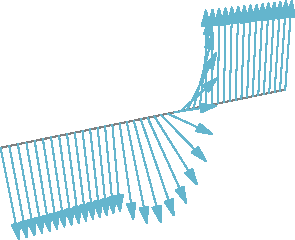
\includegraphics{figures/blochwall.pdf}
  \caption{\itshape Ejemplo de pared de Bloch.}
  \label{fig:blochwall}
\end{marginfigure}

Consideremos una pared de Bloch (figura \ref{fig:blochwall}), y razonemos sobre su grosor.
A partir del hamiltoniano de Heisenberg $U=2J\symbf{S}_1\symbf{S}_2$
se obtiene la energía de canje para los dos espines:
\begin{equation}
  ω_\mathit{ex} =2JS_1S_2\cos(φ) ∼ JS^2φ^2
\end{equation}
con $φ$ el ángulo entre los espines y $J$ la integral de canje, tras
emplear $\cos φ ∼ 1 + \oh φ^2$ para ángulos pequeños y redefinir el
origen de energías. El cambio es de $π$ radianes en $N$ pasos, luego $φ = π/N$:
\begin{equation}
  ω_\mathit{ex} = JS^2(π/N)^2
\end{equation}
La energía de canje total será $Nω_\mathit{ex} =
JS^2π^2/N$. Suponiendo una red cúbica, tenemos $1/a^2$ líneas de
átomos perpendiculares a la pared, de forma que podemos definir la
energía de canje por unidad de area de pared como
\begin{equation}
  σ_\mathit{ex} = \frac{1}{a^2} Nω_\mathit{ex} = \frac{JS^2π^2}{Na^2}
\end{equation}

La pared se expandiría sin límites si no fuera por la energía de
anisotropía, que es grande para los espines rotados de la pared.
Podemos aproximar la energía de anisotropía como la anchura $Na$ de la
pared salvo por una constante $K$, quedando la energía total de la
pared como
\begin{equation}
  E_\mathit{w} = σ_\mathit{ex} + σ_\mathit{anis} =
  \frac{JS^2π^2}{Na^2} +KNa
\end{equation}

Si minimizamos esa energía en función de $N$, obtenemos
\begin{equation}
  N_\textit{min} = \sqrt{\frac{π^2JS^2}{Ka^3}}
\end{equation}

Si la energía de anisotropía, proporcional a $K$, es alta, las paredes
serán estrechas para minimizar el número de electrones ``mal
colocados''. Si la energía de canje es alta, la pared crece para
minimizar el número de electrones no alineados y minimizar el ángulo
entre ellos. Estas dos energías compiten entre ellas para determinar
el grosor de la pared.

\chapter{Superconductividad}

\begin{marginfigure}
  \centering
  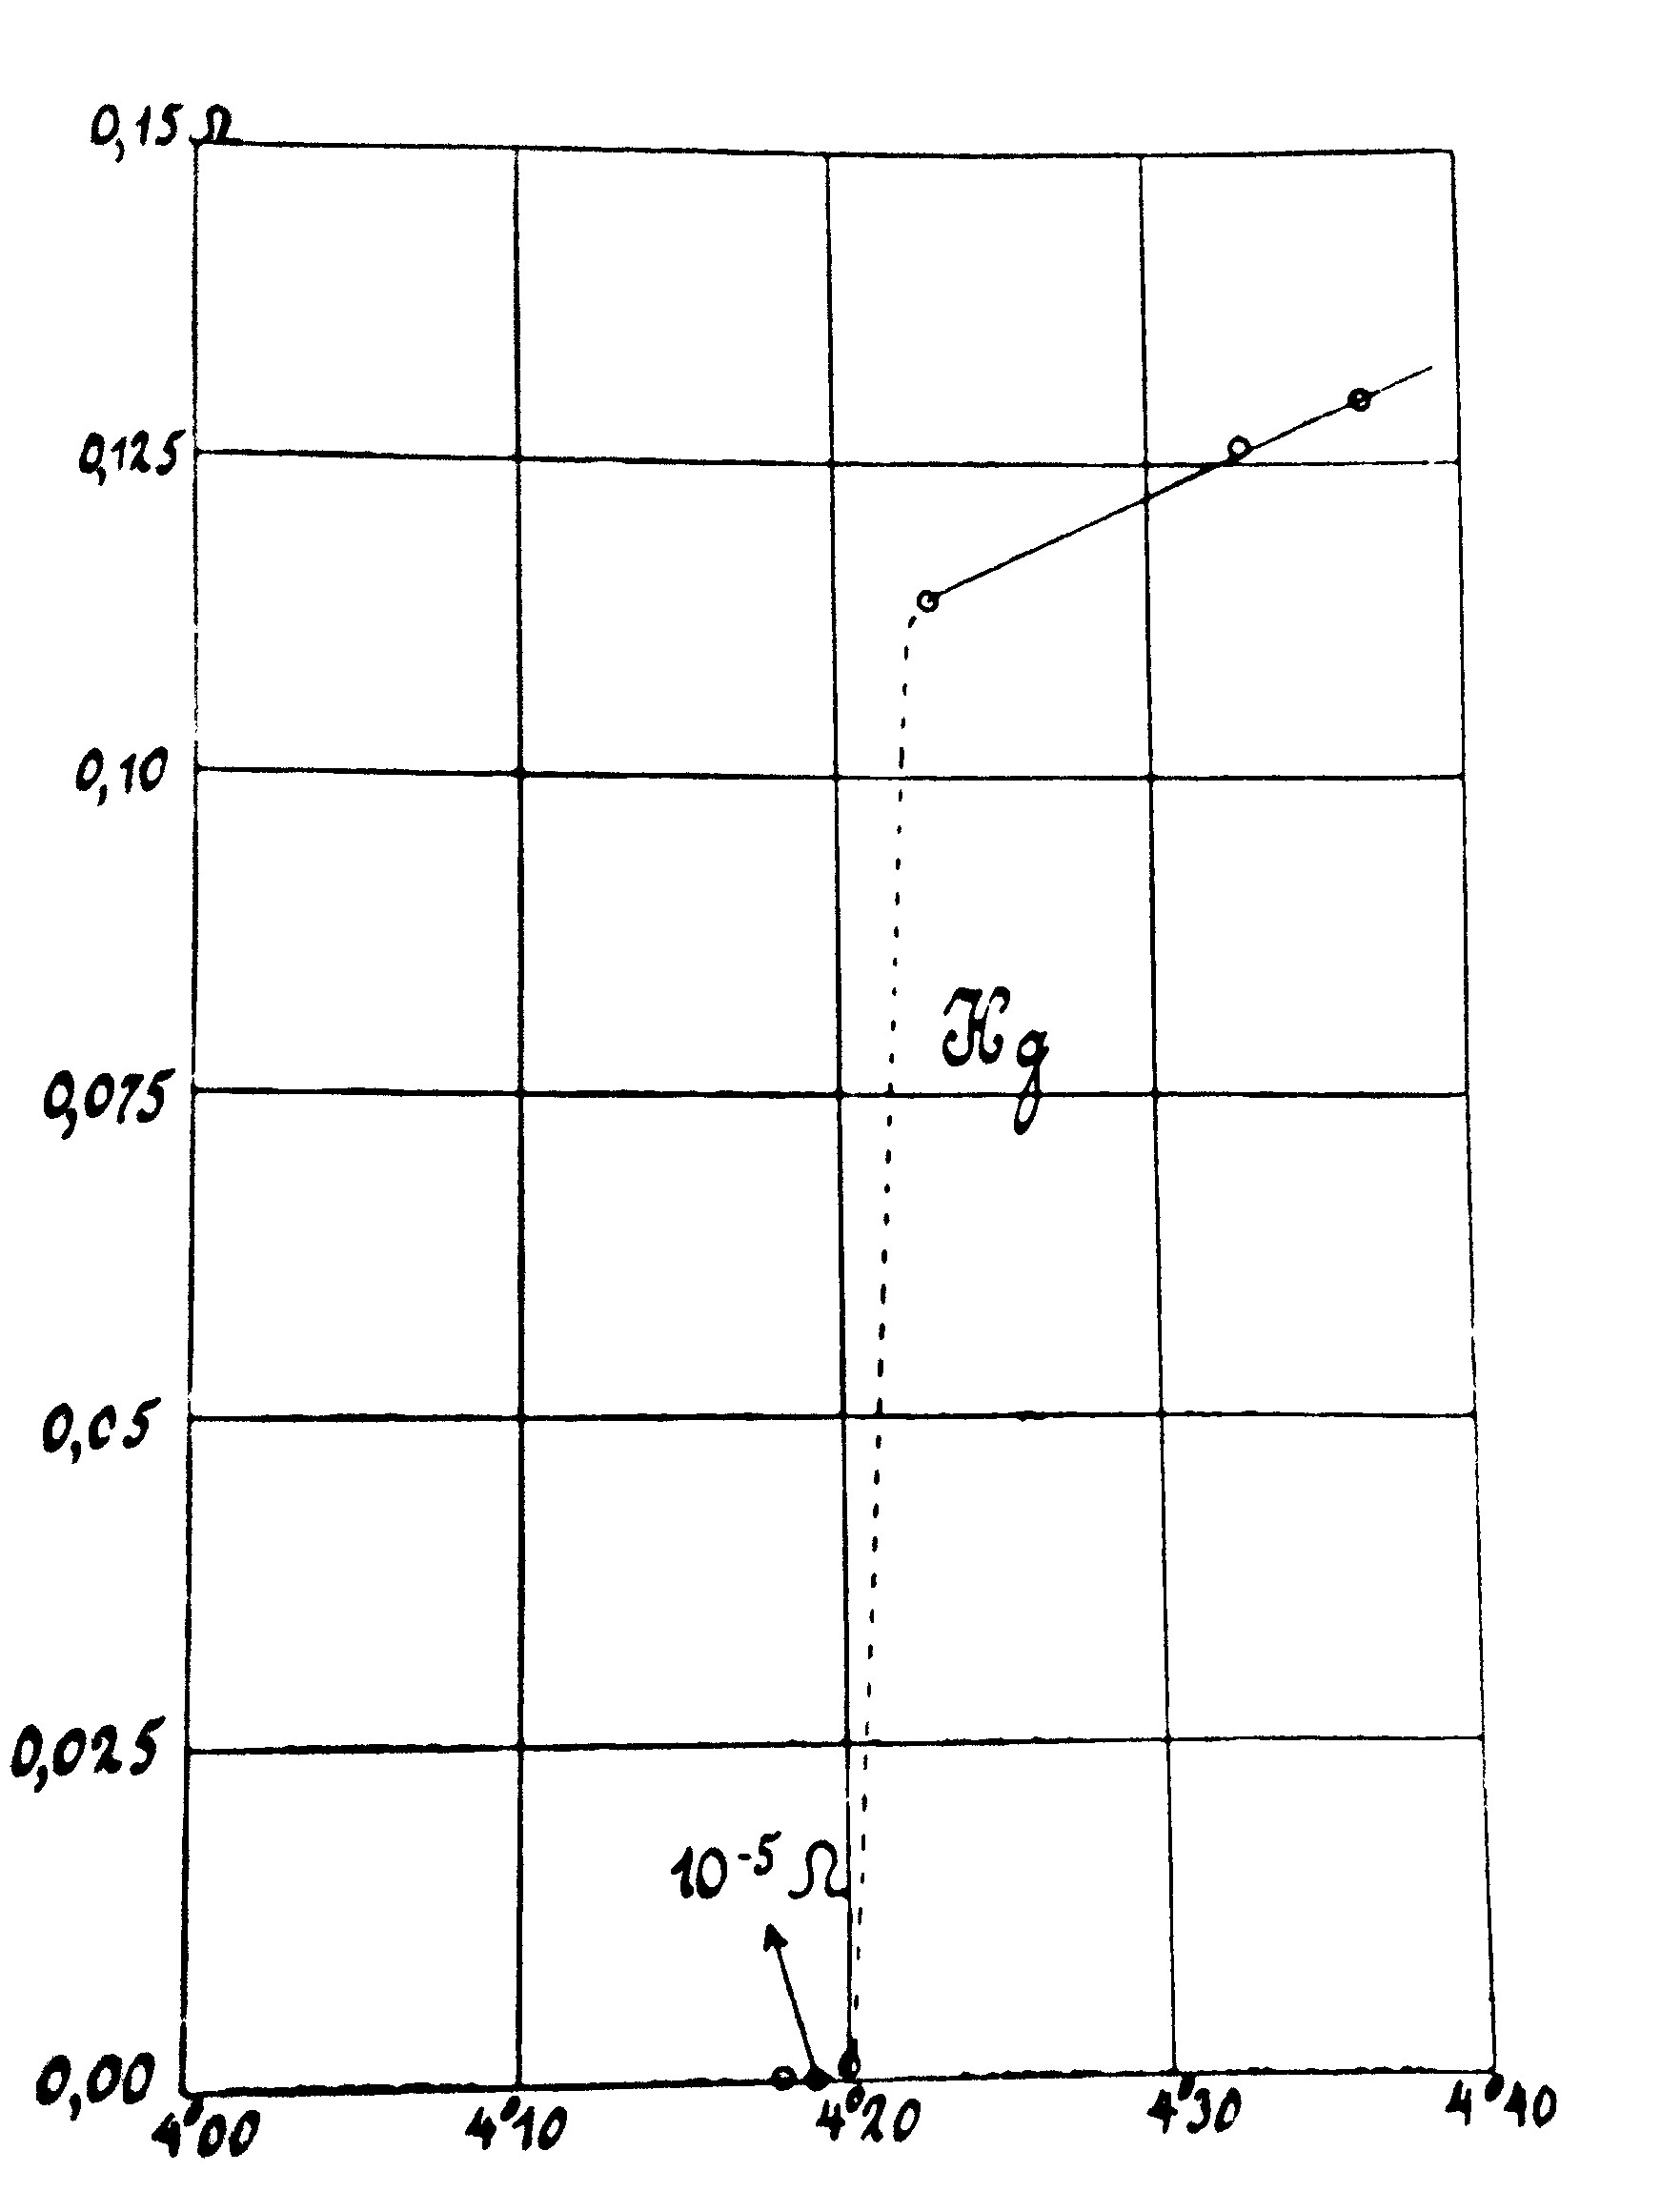
\includegraphics[width=\textwidth]{figures/smoothkamerlingh.jpg}
  \caption{\itshape Resistencia en ohmnios del mercurio frente a la temperatura
  absoluta. Esta preciosa gráfica a mano de Kamerlingh Onnes fue la
  primera observación de la superconductividad. Prestar atención a la
  belleza del $0.075$ del eje vertical.}
  \label{fig:smoothkamerlingh}
\end{marginfigure}

La resistencia de algunos compuestos se anula de forma brusca cuando
se enfrían a temperaturas suficientemente bajas, del orden de la del
helio líquido($\SI{4.2}{\kelvin}$. Este fenómeno se denota
\emph{superconductividad}, y esta caracterizado por tres propiedades:

\begin{itemize}
\item \textit{Resistencia nula} por debajo de una temperatura crítica.
\item \textit{Exclusión del flujo} de líneas de campo del interior del
  conductor, o \emph{efecto Meissner}. Es un fenómeno púramente
  cuántico, en el que el material se comporta como un diamagnético
  perfecto de $χ=-1$.
\item \textit{Un gap semiconductor}, simétrico respecto a la energía
  de Fermi y mucho más estrecho que el \textit{gap} semiconductor.
\end{itemize}

% Mon May 15 08:15:52 CEST 2017

De forma general, los superconductores se pueden clasificar en dos clases.

\begin{description}
\item[Tipo I] La transición del estado normal al semiconductor es
  abrupta, y se define mediante una temperatura de transición
  $T\sub{C}$. Repelen por completo las líneas de campo.
\item[Tipo II] La transición es progresiva, y se produce entre por dos
  temperaturas críticas. En ellos, algunas líneas de campo pueden
  penetrar en el material; tras pasar por la segunda temperatura
  crítica nada de flujo penetra, como en los de tipo I.
\end{description}

La presencia de campos magnéticos intensos puede destruir este efecto;
el valor umbral del campo se denota $H\sub{C}(T)$ y es nulo para la
temperatura crítica.

\section{Efecto Meissner}
Las propiedas magnéticas de los superconductores son tan
\textit{ósom} como las eléctricas, y no se pueden explicar
suponiendo que estos materiales son conductores típicos con
resistencia nula. Meissner y Ochsonfeld encontraron que si un
superconductor se enfría por debajo de su $T\sub{C}$ mientras se
aplica un campo $B$, en la transición superconductora este expulsa las
líneas de flujo. A continuación veremos que esto contradice las
predicciones de la electrodinámica clásica.

En un conductor normal se verifican la ley de Ohm y las relaciones de
Maxwell, en concreto:
\begin{align}
  \symbf{E} = ρ \symbf{J}\qquad \pdv{\symbf{B}}{t}=-∇×\symbf{E}
\end{align}

De la ley de Ohm deducimos que si $ρ→0$ con $\symbf{J}$ finita,
entonces $\symbf{E}$ necesariamente se anula. Si llevamos este
resultado a la ley de Maxwell $\dot{\symbf{B}}=-∇×\symbf{E}$, vemos
que el campo magnético en el material ha de mantenerse constante. No
obstante, los resultados experimentales contradicen este resultado: el
campo magnético se expulsa al bajar la temperatura por debajo de
$T\sub{C}$, variando hasta $B=0$.

Para entender el efecto Meissner, consideremos una muestra constituída por
un cilindro hueco cuyo eje es paralelo a $\symbf{B}$, que se lleva
por diferentes caminos (figura \ref{fig:paths}) a través de su
transición superconductora.

\begin{marginfigure}
  \centering
  \begin{tikzpicture}[scale=3]
    \draw[->] (0,0) -- (1.5,0) node[at end, below] {$T$};
    \draw[->] (0,0) -- (0,1.1) node[at end, left] {$B$};
    \draw[-|] (0,0) -- (0,0.5) node[at end, left] {$B\sub{R}$};
    \draw[PlotDefault, thick] (0,1) to[out=0,in=100] (0.75,0);
    \draw[dashed,->] (1,0) -- (1,0.25); \draw[dashed] (1,0.25) -- (1,0.5);
    \draw[dashed,->] (0.5,0) -- (0.5,0.25); \draw[dashed] (0.5,0.25) -- (0.5,0.5);
    \draw[dashed,->] (1,0) -- (0.75,0); \draw[dashed] (0.75,0) -- (0.5,0);
    \draw[dashed,->] (1,0.5) -- (0.75,0.5); \draw[dashed] (0.75,0.5) -- (0.5,0.5);
    \node[above left] at (0.5,0.5) {R};
    \node[below left] at (0.5,0) {S};
    \node[above right] at (1,0.5) {Q};
    \node[below right] at (1,0) {P};
  \end{tikzpicture}
  \caption{Diagrama de fases de una muestra superconductora.}
  \label{fig:paths}
\end{marginfigure}

\textit{Si seguimos P→Q→R}, el cilindro se somete primero a un campo
magnético $B\sub{R}$ y después se enfría hasta el estado
superconductor. El campo en el interior del cilindro antes de
atravesar la línea de transición es $B\sub{R}$ tanto dentro como fuera
del cilindro. Al atravesar la línea, el campo externo se expulsa, de
forma que el campo interno sigue siendo $B\sub{R}$ aunque se varíe el
valor del campo externo posteriormente: el interior del cilindro
superconductor está aislado de dichas variaciones por el efecto
Meissner\footnote{Para profundizar más en cómo el ser superconductor
  conduce a este apantallamiento, ver
  \url{http://tinyurl.com/physicsbatman}}. Notar que esto implica una
corriente interna de valor $-B\sub{R}/μ_0$ que no se disipa y compensa
el campo externo, y por lo tanto un almacenamiento de energía.

\textit{Si en cambio realizamos P→S→R}, primero la muestra se enfría
hasta el estado superconductor con $B=0$ dentro y fuera, y luego se le
aplica un campo $B\sub{R}$. El campo en el interior era nulo cuando la
muestra atravesó la línea de transición, y lo seguira siendo aunque se
aumente en S→R, debido al apantallamiento del efecto Meissner. Notar
como el camino diferente da lugar a una situación diferente que P→Q→R,
a pesar de que el punto inicial (P) y el final (R) son el mismo.

El material superconductor (las paredes del cilindro) siempre tiene
$B=0$ cuando está en la fase superconductora.

\section{Gap superconductor}
El \textit{gap} energético de los superconductores ($∼\SI{1}{\milli\eV}$) es
mucho más pequeño que el de los semiconductores ($∼\SI{1}{\eV}$), y de
naturaleza completamente distinta. En los aislantes, está causado por
la interacción de los electrones con la red. En los superconductores,
el mecanismo principal es la ligadura de electrones con otros
electrones formando \emph{pares de Cooper}, y jugando la red
\marginnote{
\includegraphics[width=0.2\textwidth]{figures/koopa.png}}
únicamente un papel indirecto. Además, sólo existe por debajo de la
temperatura crítica en estos últimos.
El \textit{gap} es simétrico respecto a la temperatura de Fermi, y fue medido
experimentalmente por Giaver (1960) en un ``sandwich''
metal-aislante-superconductor de capas ultrafinas.

Si se establece un $ΔV$ entre el metal y el semiconductor, los
electrones sólo pueden cruzar por efecto tunel. Para $ΔV$ pequeño, no
se detectaba corriente túnel, empezando a aparecer para cierto valor
$±V_0$ (figura \ref{fig:ohmnicmyass}). A partir de dichos valores, el
comportamiento es ohmnico. Esto sugiere la existencia de un \textit{gap} de
anchura $2V_0$, que
queda perfectamente caracterizando teniendo en cuenta que la derivada
de la corriente túnel es proporcional a la densidad de estados.

\begin{marginfigure}
  \centering
  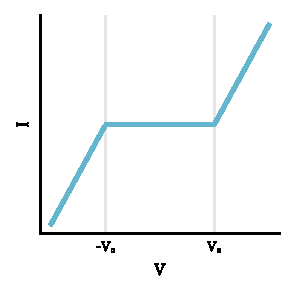
\includegraphics{figures/ohmnicmyass.pdf}
  \caption{\itshape Corriente túnel en un ``sandwich'' de capas ultrafinas
    metal-aislante-superconductor.}
  \label{fig:ohmnicmyass}
\end{marginfigure}

La anchura del \textit{gap} disminuye al aumentar la temperatura, ya
que la agitación térmica de los electrones les facilita superar la
barrera de potencial del semiconductor.

\section{Ecuación de London}
En secciones anteriores se ha achacado a la existencia de
\emph{supercorrientes} en la superficie del superconductor la
expulsión del flujo magnético del su interior se puede tratar de
analizar estas corrientes mediante electrodinámica clásica.

Partamos de la ley de Ohm, $\symbf{J}=σ\symbf{E}$. London propuso
modificarla de forma que la densidad de corriente $\symbf{J}$ fuera
proporcional al vector $\symbf{A}$ del campo magnético local:
\marginnote{Recordar que $\symbf{B}=∇×\symbf{A}$.}
\begin{equation}
  \symbf{J} = \frac{-1}{μ_0λ\sub{L}^2} \symbf{A}
\end{equation}
donde la constante de proporcionalidad se justificará posteriormente.
Este postulado se conoce como \emph{ecuación de London}, y también
puede expresarse como
\begin{equation}
  ∇×\symbf{J} = \frac{-1}{μ_0} \symbf{B}
\end{equation}
De las leyes de Maxwell conocemos que $∇×\symbf{B}=μ_0 \symbf{J}$,
tomado el rotacional a ambos lados de esta expresión concluímos que
\begin{equation}
  \begin{split}
    ∇×(∇×\symbf{B}) &= μ_0∇×\symbf{J} \\
    \cancelto{0}{∇(∇⋅\symbf{B})} - ∇^2 \symbf{B} &= μ_0∇×\symbf{J}\\
    ∇^2 \symbf{B} &= \frac{\symbf{B}}{λ\sub{L}^2}
  \end{split}
\end{equation}
donde se ha sustituído $∇×\symbf{J}$ con la ecuación de London,
$∇×\symbf{J} = \frac{-1}{μ_0} \symbf{B}$, y se han usado propiedades
oscuras del operador $∇$ de esas que nos enseñaba Esteve. La ecuación
no admite soluciones uniformes en el espacio excepto por $B=0$, de
forma que $B=\text{cte.}$ no es posible. La única solución es un campo
$B=B_0 e^{-x/λ\sub{L}}$ con decaimiento exponencial, de forma que
identificamos $λ\sub{L}$ con la \emph{longitud de penetración de
  London}. Es un parámetro medible experimentalmente que indica la
distancia que penetra el campo externo en el superconductor, y cobra
especial relevancia en el estudio de los de tipo II.

Es posible\footnote{Quiero mi cinco.} estimar teóricamente su valor.
La expresión habitual para la densidad de corriente es $\symbf{J}=nq
\symbf{v}$, donde $n$ es la concentración de portadores (pares de
Cooper) y $q=-2e$ su carga. Bajo un campo magnético caracterizado por
un potencial vector $\symbf{A}$, la velocidad $\symbf{v}$ se relaciona
con el momento total de los portadores mediante
\begin{equation}
  \symbf{p} = m \symbf{v} + \frac{q}{c} \symbf{A}
\end{equation}
de forma que
\begin{equation}
  \symbf{v} = \frac{1}{m} \left( \symbf{p}-q \symbf{A} \right)
\end{equation}
Esto nos permite reescribir la expresión para la densidad de corriente
$\symbf{J}$ como
\begin{equation}
  \symbf{J} = \frac{nq}{m} \symbf{p} - \frac{nq^2}{m} \symbf{A}
\end{equation}
Igualando dicha $\symbf{J}$ con la $\symbf{J} =
-\symbf{A}/μ_0λ\sub{L}^2$ hallada para la ecuación de London, se
obtiene
\begin{equation}
  λ\sub{L} = \sqrt{\frac{m}{μ_0nq^2}}
\end{equation}

% Wed May 17 09:07:41 CEST 2017
\section{Aspectos básicos de la teoría BCS}
Es la teoría más completa en la actualidad, abarcando un amplio rango
de superconductores. En ella las funciones de onda describen
cuasipartículas constituídas por parejas de electrones, los pares de
Cooper ya nombrados. Están caracterizados por $Q=-2e$, y sus
electrones poseen $S_1=-S_2$ y $\symbf{k}_1=-\symbf{k}_2$.

La red juega un paper % Pun intended
indirecto en crear estas parejas. Un electrón desapareado deforma la
red, y otro aprovecha esta deformación para disminuir su energía; la
distancia a la que estos electrones se correlacionan viene dada por $ξ$.

Esta unión también recibe el nombre de \emph{emparejamiento de onda
  S}. Las funciones de onda BCS permiten justificar algunos hechos de
la superconductividad:
\begin{itemize}
\item Una interacción atractiva entre electrones conduce a un estado
  fundamental separado de los excitados por un \textit{gap} energético. El
  campo crítico $H\sub{C}$, las propiedades térmicas, y la mayoría de
  las propiedades electromagnéticas son consecuencia de la existencia
  de este \textit{gap}.
\item El \textit{gap} energético de la interacción e \textsuperscript{-}→red→e\textsuperscript{-}
  tiene una magnitud consistente con la observada.
\item Se predice la existencia de dos escalas de longitud, dadas por
  la penetracíón de $B$ en el material ($λ\sub{L}$) y la longitud de
  correlación $ξ$ de los pares de Cooper.
\item El flujo magnético en un anillo conductor está cuantizado, y su
  unidad efectiva de carga es $2e$ en lugar de $e$.
\end{itemize}

\subsection{Longitudes características}
La ecuación de London presenta un carácter local, mientras que la
descripción de los superconductores requiere introducir la
\emph{longitud de correlación electrónica} $ξ$ ya vista para
caracterizar el rango sobre el que debería promediarse $\symbf{A}$ a
la hora de obtener $\symbf{J}$. También es una medida del grosor
mínimo que debe tener la capa de transición entre un material normal y
uno superconductor.

Una modulación de la función de ondas\footnote{Suponemos que es
  plana.} del electrón requiere de un aporte de energía cinética
externa; denominando a $q$ al número de ondas de la onda modulante, se
requiere\footnote{La energía va como $k^2=k⋅k∼k⋅q$.}
\begin{equation}
  E_k = \frac{ℏ^2kq}{2m}
\end{equation}
Si esta energía es mayor que la $E_g$ del \textit{gap}, la
superconductividad se destruye. Hallamos el valor crítico $q_0$
despejando de la ecuación anterior con $E_k = E_g$:
\begin{equation}
  \frac{ℏ^2}{2m}k\sub{F}q_0 = E_g
\end{equation}
donde se ha tomado $k=k\sub{F}$ ya que prácticamente todos los
electrones están en el nivel de Fermi. A partir de esta modulación se
define la \emph{longitud de correlación intrínseca}:
\begin{equation}
  ξ_0 = \frac{1}{q_0} = \frac{ℏ^2k\sub{F}}{2mE_g} = \frac{ℏ^2v\sub{F}}{2E_g}
\end{equation}

Pippard también halló un valor para $ξ_0$ considerando que únicamente
las energías del orden de $\kb T\sub{C}$ podían ser responsables
de fenómenos que tuviesen lugar a temperaturas por debajo de
$T\sub{C}$; únicamente los electrones dotados de la \emph{velocidad de
Fermi}, $v\sub{F}$, se ven involucrados.\footnote{Son los que están
cerca del gap, teniendo $E∼E\sub{F}$.}

Bajo esta hipótesis, el rango de valores del momento permitidos es del
orden de $δp∼\kb T\sub{C}/v\sub{F}$. El principio de incertidumbre
nos da una longitud asociada:
\begin{equation}
  δx ≳ \frac{ℏ}{δp} = \frac{ℏ^2v\sub{F}}{\kb T\sub{C}} ∼ ξ_0
\end{equation}

La longitud de correlación intrínseca $ξ_0$ apareció por primera vez
en las \emph{ecuaciones de Landau-Ginzburg}, derivadas de la teoría
BCS. Describen la zona de transición entre un material superconductor
y uno normal. Tanto $ξ_0$ como $λ\sub{L}$ son parámetros intrínsecos
cuyos valores reales $ξ, λ$ son diferentes a los teóricos. En
particular, $ξ<ξ_0$ y $λ > λ\sub{L}$, estando los parámetros
condicionados por el recorrido libre medio $ℓ$ de los electrones en el
material, medido en el estado normal.

En el \emph{dirty limit}, cuando $ℓ$ es muy pequeño por estar el
material altamente impurificado, se puede aproximar
\begin{equation}
  ξ ≃ \sqrt{ξ_0ℓ} \qquad λ ≃ λ\sub{L} \sqrt{\frac{ξ_0}{ℓ}}
\end{equation}

Al cociente $κ≃λ/ξ≃λ\sub{L}/ℓ$ se le denota \emph{parámetro de Landau-Ginzburg}.

\marginnote[-2cm]{
  \begin{flushright}
    \slshape ``Las redes tienen un efecto muy importante y por lo
    tanto la masa. Y eso además se supo porque la primera observación
    no se encontraba por qué un material que parámetro característico
    de un material fuera superconductor. Hasta que alguien notó que
    estaba relacionada con la masa.''
  \end{flushright}
  --- \textsc{Paulo Coelho}
}

\section{Superconductores tipo II}

Justifiquemos la existencia de una región de transición en los
superconductores tipo II. Nos basamos en un criterio energético,
encontrando que la penetración del campo magnético es energéticamente
favorable.

En los materiales de tipo I $λ≪ξ$, mientras que en los de tipo II
$λ≫ξ$. Consideremos las dos contribuciones principales a la energía:
\begin{itemize}
\item \textit{La energía magnética} es cero en el estado normal (N) y
  aumenta hasta $B\sub{C}^2/2μ_0$ en el superconductor
  (S).\footnote{Viene de integrar la energía de Gibbs, que va como $B \dd{B}$.}
  El cambio ocurre en una región de
  longitud $λ$.
\item \textit{La energía de los electrones} es más baja en el estado S
  debido a la energía de condensación asociada a la formación de pares
  de Cooper. El cambio ocurre en una región de grosor $ξ$.
\end{itemize}

Ambas energías se balancean (figura \ref{fig:balance}), dando lugar a
un punto de equilibrio, estable o inestable en función del tipo de
superconductor. Únicamente en los de tipo II generar una zona de
transición es energéticamente favorable.

\begin{marginfigure}
  \centering
  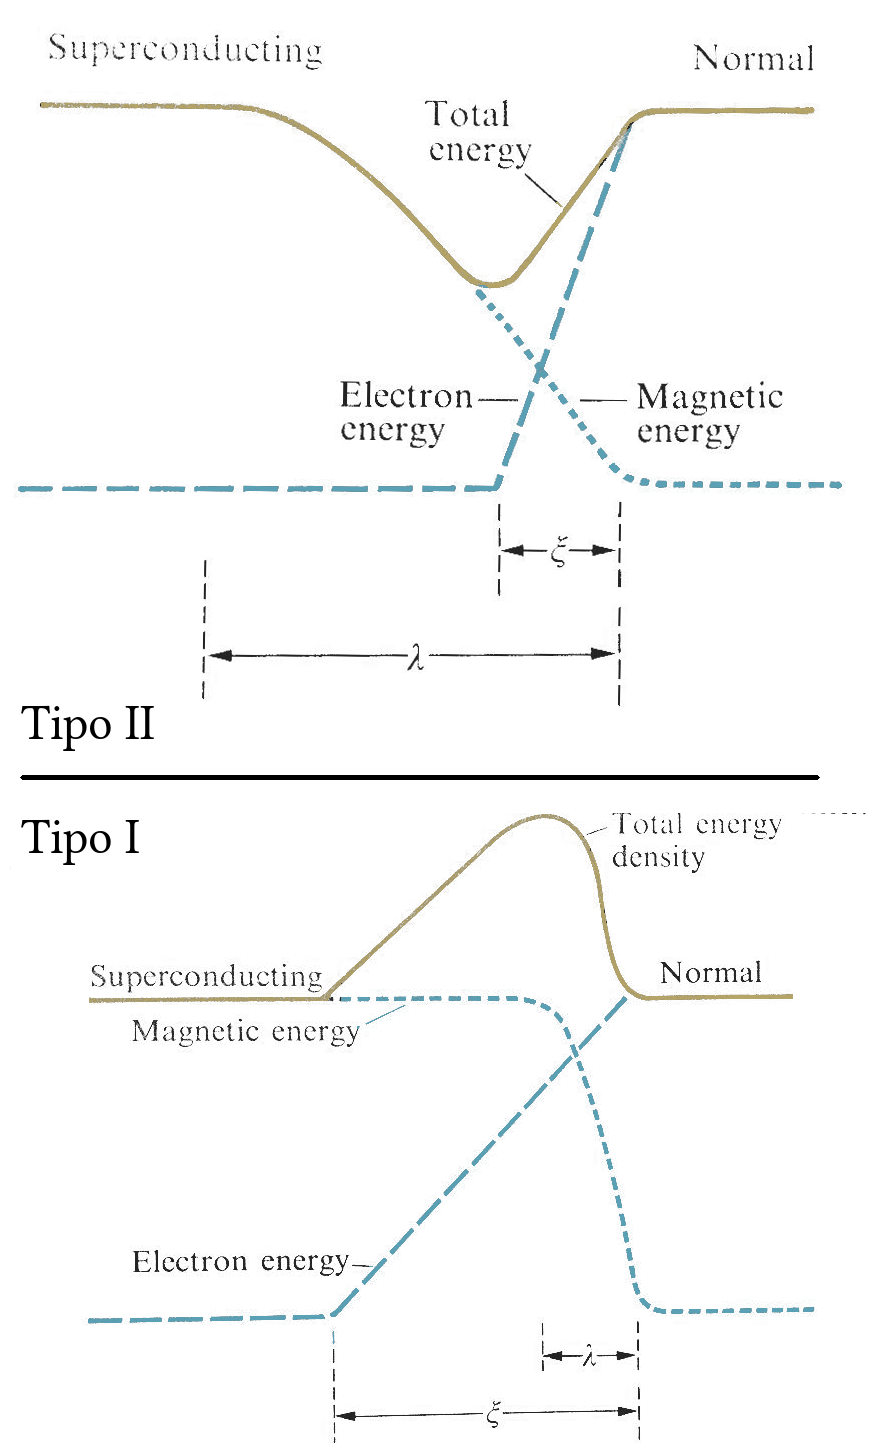
\includegraphics[width=\textwidth]{figures/tipos.png}
  \caption{\itshape Energías involucradas en la creación de una barrera
    normal-semiconductor. En los superconductores tipo I la barrera es
    energéticamente desfavorable.}
  \label{fig:balance}
\end{marginfigure}

\subsection{Cuantización del flujo}

% Mon May 22 09:31:09 CEST 2017

% Bleany kickin' it
Dentro de un superconductor como el cilindro hueco visto anteriormente
existen supecorrientes en las superficies, que se atenúan conforme nos
adentramos en el material. La corriente consiste en un flujo de pares
de Cooper, cada uno con un vector de ondas $\symbf{k}$ y un momento
$\symbf{p}=ℏ \symbf{k}$, que debe cumplir la \emph{regla de
  cuantización de Bohr-Sommerfeld}:
\begin{equation}
  \oint \symbf{p} \dd{\symbf{s}} = N h
\end{equation}
con $h$ la constante de Plank y $N∈\mathbb{Z}$, estando la integral
definida sobre un \textit{loop} de corriente. Sustituyendo
$\symbf{p}=m \symbf{v}+ q \symbf{A}$,
\marginnote{$\symbf{J}= n q \symbf{v}$}
\begin{equation}
  \begin{split}
    Nh &= \oint (m \symbf{v} + q \symbf{A} ) \dd{s} \\
    &= \oint \frac{m}{nq} \symbf{J} \dd{s} + \oint q \symbf{A} \dd{s}
  \end{split}
\end{equation}

En puntos del interior del metal $\symbf{J}=0$, anulándose la primera
integral. Identificando\footnote{$\oint \symbf{A} \dd{s} = \iint ∇×
  \symbf{A} \dd{S} = \iint \symbf{B} \dd{S}$} la segunda integral con
el flujo $Φ$ a través del \textit{loop} de corriente, vemos que
\begin{equation}
  \abs{Φ} = N \abs{\frac{h}{2e}} = NΦ_0
\end{equation}
sustituyendo $q$ con la carga $-2e$ de un par de Cooper. Hemos
obtenido que el flujo está cuantizado en unidades de $Φ_0$, muy
pequeñas y difíciles de observar.

\subsection{Vórtices}
\marginnote{Notar que este efecto sólo ocurre entre los dos $H$ de
  transición del superconductor.}
La penetración de flujo característica de los superconductores tipo II
se produce mediante estructuras tubulares llamadas \emph{vórtices},
dentro de las cuales el material no es superconductor. Están
dispuestos en una red triangular (\emph{red vorticial de Abrikosov})
cuya escala de longitud viene dada por $λ\sub{L}$,
siendo su colocación es independiente de la red cristalina.

La densidad de corriente y el número de pares de Cooper disminuye al
adentrarnos en ellos.


\section{Reflexiones de Andreev}

\begin{marginfigure}
  \centering
  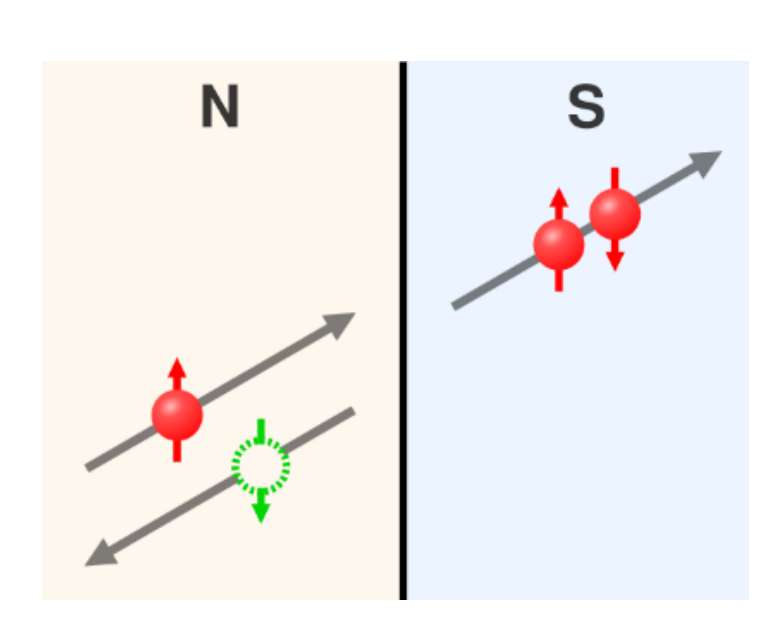
\includegraphics[width=\textwidth]{figures/andreev.png}
  \caption{Unión metal-superconductor experimentando una reflexión de Andreev.}
  \label{fig:andreev}
\end{marginfigure}

Supongamos una unión metal-superconductor en la que se aplica una
diferencia de potencial. Si el $ΔV$ es mayor que el \textit{gap} del
superconductor los electrones circularán por él, con una conductancia
$G$. Si en cambio $ΔV$ es del orden del \textit{gap}, los electrones
que se adentren en la banda prohibida han de formar necesariamente
pares de Cooper. Esto fuerza a un segundo\footnotemark electrón a
cruzar o, de forma equivalente, a un hueco a venir de la zona
superconductora, de forma que la conductancia sube a $2G$.
\footnotetext{Recordar que en un superconductor \emph{no} hay
  electrones desapareados.}

Debido a las características de los pares de Cooper, el segundo
electrón ha de tener espín opuesto. Si el material normal tiene toda
la banda polarizada en la misma dirección (\emph{full spin
  polarization}) no podrá aportar el segundo electrón, y la
conductancia caerá a cero en lugar de crecer.

\chapter{Nanociencia}

Las propiedades de los materiales eléctricos y magnéticos estudiados
hasta ahora presentan cambios muy importantes cuando el tamaño del
sistema que constituyen se reduce mucho (hasta la escala de los
nanometros). La nanociencia y la nanotecnología son las disciplinas
encargadas de caracterizar y describir estas nuevas propiedades, así
como de encontrar aplicaciones útiles para las mismas. La aparición de
la nanotecnología viene con la era cuántica, cuyo inicio puede
fecharse en 1897 cuando J.\,J.\,Thomson descubre el electrón.
Posteriormente Max Planck pondría la primera piedra en el camino al
presentar la cuantificación de la radiación térmica en 1918; seguido
por la presentación del fotón como cuanto electromagnético por
Einstein en 1920. En 1929 de Broglie propuso la hipótesis ondulatoria;
y en 1932 Heisenberg dio coherencia a todo lo anterior sentando las
bases de la mecánica cuántica.

La nueva era cuántica venía condicionada por la instrumentación
disponible. El microscopio óptico, utilizado hasta entonces, estaba
limitado por la longitud de onda de la luz; pudiendo obtener
resoluciones de hasta el orden de los µm. En 1933 se inventó el
microscopio electrónico; que utilizaba radiación de electrones en vez
de luz visible. La diferencia fundamental es que la longitud de onda
asociada a los electrones depende del voltaje de aceleración al que
éstos sean sometidos; lo cual permite alcanzar resoluciones mucho
mayores que el microscopio óptico. En 1986, Binning y Rhorer
inventaron el microscopio de sonda local por efecto túnel; abriendo
todo un abanico de nuevas posibilidades en el campo de la microscopía.

\section{Nanopartículas}

Tenemos, en varias dimensiones, partículas (3D), \textit{thin films}
(2D), nanohilos (1D) y puntos cuánticos (0D). Conforme bajamos las
dimensiones, la densidad de estados parabólica se va aproximando a
deltas de Dirac con niveles energéticos discretos.

La parte activa de los materiales suele ser la superficie, que es un
porcentaje mayor de los átomos conforme disminuimos el tamaño. Esto es
vital, por ejemplo, en catalizadores, donde la nanotecnología juega un
papel importante.

\begin{margintable}
  \begin{tabular}{lcc}
    \toprule
    Capas atómicas & Átomos & Superficie (\%) \\
    \midrule
    1              & 13     & 92               \\
    2              & 55     & 76               \\
    3              & 147    & 36               \\
    4              & 309    & 52               \\
    5              & 561    & 45               \\
    6              & 1415   & 35               \\
    \bottomrule
  \end{tabular}
\end{margintable}

El crecimiento de \textit{thin films} es extraordinariamente
complicado, ya que se hace que las capas se depositen átomo a átomo. A
esto se le denomina \emph{crecimiento epitaxial}.


\section{Espectroscopía}
\marginnote{Las energías de las partículas incidentes o salientes se puede estimar
con el tiempo de vuelo (neutrones) o mediante selección por un prisma
magnético (electrones).}
Para poder analizar una muestra en el microscopio electrónico de
transmisión, es necesario que tenga un grosor máximo de unos pocos
nanómetros. Es especialmente interesante analizar los rayos X
generados por la muestra.

\begin{flushleft}
  \textbf{Nota de examen}: \emph{nunca} se dice que en TEM los
  electrones sufren difracción en la muestra, sufren \emph{scattering}.
\end{flushleft}

% Tutoría viernes a las 10:30

% Mon May 29 08:01:00 CEST 2017

\section{Nanopartículas}
El tratamiento de enfermedades con nanopartículas es un tema
\textit{jot}. Una vía de administración es el uso de virus decorados
con nanopartículas magnéticas.

Llamamos \emph{sistemas nanoparticulados} a sistemas con partículas
por debajo de los \SI{100}{\nano\metre} de diámetro.
Un campo grande de investigación hoy en día es el recubrimiento de
nanopartículas con otros materiales; un método elegante es mediante
evaporación (\emph{plasma de Krästchmer-Hoffman}).

En partículas pequeñas, el efecto de la anisotropía magnetocristalina
se hace muy pequeño. A este límite (por debajo de los
\SI{25}{\nano\metre}) se le llama \emph{superparamagnético}, y esta
caracterizado por no estar el momento magnético fijo en una dirección
cristalográfica.

\marginnote{
  \begin{flushright}
    \textit{
      ``It can't be bargained with, it can be reasoned with. It doesn't
      feel pain, or remorse, or fear and it absolutely will not stop,
      EVER, until you have voted.''
    }
  \end{flushright}

  --- \textsc{A Student, on the Ibarraton}
}

Si la partícula es muy pequeña, sólo tiene un dominio magnético. El
campo coercitivo desaparece en esta situación. Pasa de tener un ciclo
de histéresis a no tenerlo, como en un material paramagnético.

El comportamiento del campo coercitivo con el tamaño no es trivial. En
lugar de aumentar monótonamente con el tamaño, tiene un máximo para un
diámetro $D_s$, para despues tender asintóticamente a un valor para
$L→∞$ (figura \ref{fig:hcwithsize}).

\begin{marginfigure}
  \centering
  \begin{tikzpicture}[scale=3]
    \draw[->] (0,0) --(1.5,0) node[below, at end] {Diámetro};
    \draw[->] (0,0) --(0,0.6) node[left, at end] {$H\sub{C}$};
    \draw[thick, PlotDefault] (0.05,0) to[out=75, in=180] (0.4,0.5) to[out=0, in=180] (1.25,0.2);
  \end{tikzpicture}
  \caption{\itshape El campo coercitivo depende del tamaño de las nanopartículas.}
  \label{fig:hcwithsize}
\end{marginfigure}

Otra característica de estos \emph{supermomentos} es que siguen la ley
de Langevin.
Además, tienen un comportamiento $H/T$ universal y fluctúan entre dos
estados de magnetización. La fluctuación depende de $t$ y viene
descrita por la \emph{ley de Arrhenius}, que regula el comportamiento
de estos sistemas bajo una barrera energética. El tiempo
característica para un \emph{magnetization reversal} es
\begin{equation}
  τ = τ_0 e^{-βKV}
\end{equation}
Esto es relevante en discos duros. Si se aumenta la densidad de
información esta $τ$ disminuye, haciendo que el sistema pierda fiabilidad.

% Tue May 30 09:05:11 CEST 2017
\subsection{Magnetic hyperthermia}
Cuando las partículas son suficientemente pequeñas, su capacidad para
absorber radiación (y calentarse) cambia. Esto es especialmente
interesante en el tratamiento de cánceres, donde se llevan las
nanopartículas al tumor para a continuación calentarlo y destruirlo.

Existen dos mecanismos, la \emph{rotación Browniana} (movimiento
físico de las nanopartículas) y la \emph{Neel relaxation} (movimiento
del vector de imanación), que generan disipación térmica.

\section{Thin films}
\marginnote{
  \begin{flushright}
    \textit{
    ``I would build a great thin film, and nobody builds thin films
    better than me. Believe me. And I'll build it very inexpensively. I'll
    build a great, great thin film on our southern border and I will have
    Mexico pay for that thin films. Mark my words.''
    }
  \end{flushright}
  --- \textsc{Paulo Cohelo}
}

El equipo de fabricación (\emph{un maquinón}) mediante \emph{pulse
  laser deposition} (PLD) consiste en un láser pulsado de alta potencia,
que se lleva al interior de una campana donde se sitúan unos blancos,
de los que se arranca material. Como la deposición es a escala
atómica, todo el proceso se realiza en ultra alto vacío.
El proceso es tan preciso que se pueden depositar capas monoatómicas,
diseñando materiales que no existen en la naturaleza.

Otro método es el \emph{sputtering}. Los átomos se proyectan mediante
un campo electromagnético sobre el material para depositarlos.

Por último, también se puede realizar deposición mediante \emph{ion
  beam} y \emph{electron beam}. El rayo excita al substrato, que
absorbe partículas de un gas en el que está inmersa.

No hay que olvidar que los \textit{thin films} se depositan sobre un
sustrato, que hay que escoger cuidadosamente en función de la
aplicación, considerando propiedades mecánicas, red cristalográfica,
etc. Por ejemplo, al tensionar las películas se pueden obtener nuevos
fenómenos físicos y transiciones de fase.

Las multicapas pueden ser de \emph{materiales granulares}, cuando el
espesor es muy pequeño y no se tiene una ``banda'' continua de
material.

Otra técnica de deposición es la CVD, \emph{chemical vapor
  deposition}. En ella, gases no inertes reaccionan con el substrato,
recubriéndolo. Existen variantes \emph{atmospheric pressure},
\emph{low pressure}, \emph{plasma enhanced}, \emph{high density
  plasma}, \ldots



\part{Ejercicios}
\chapter*{Tema 1}
% 1.1
\begin{tcolorbox}[halign=left]
  \lettrine[lines=2]{\color{ExerciseNumberColor}1.1}{}
  \emph{ Demostrar que en simetría cúbica el campo eléctrico en un
    átomo del interior de un material es $\symbf{E}_0$, el campo externo.
  }
\end{tcolorbox}

El campo local será $\symbf{E}_0$, el campo externo, más
$\symbf{E}_1+\symbf{E}_2+\symbf{E}_3$. Por simplicidad, y sin
perder generalidad, supondremos $\symbf{E}_0 = E_0 \hat{z}$.

\begin{flushright}
  \emph{Campo de despolarización E\textsubscript{1}}
\end{flushright}

El cálculo del campo de despolarización, $E_1$, es inmediato.
\begin{equation}
  E_1 = \frac{-NP}{ε_0} = \frac{-P}{3ε_0}
\end{equation}
en dirección $\hat{z}$, y suponiendo una cavidad de Lorentz esférica
($N=\nicefrac{1}{3}$).


\begin{flushright}
  \emph{Campo de Lorentz E\textsubscript{2}}
\end{flushright}

Para calcular $E_2$, suponemos una densidad de carga esférica (figura
\ref{fig:int_geometry}) con $σ=-\symbf{P}\hat{n}=-P\cos θ$ causada
por la polarización del material.
\begin{marginfigure}
  \centering
  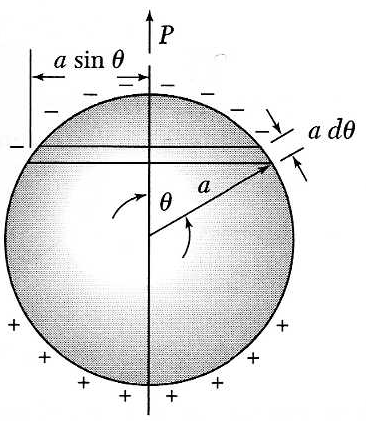
\includegraphics[width=\textwidth]{figures/int_geometry.png}
  \caption{\itshape El campo eléctrico va de las cargas positivas a las
    negativas, de forma que $\symbf{E} ∥ \hat{z}$.}
  \label{fig:int_geometry}
\end{marginfigure}

La mitad superior está cargada
negativamente, y la inferior positivamente (siguiendo el signo de
$\cos θ$), de forma que
\begin{equation}
  \dd{\symbf{E}} = \frac{-1}{4πε_0} \frac{σ \dd{\symbf{S}}}{r^2}
  = \frac{1}{4πε_0} \frac{P \cos θ \dd{\symbf{S}}}{r^2}
\end{equation}
donde $r$ es el radio de la cavidad de Lorentz. El signo menos implica
que se escogen los $\dd{\symbf{S}}$ apuntando hacia fuera de la
esfera; notar como $\hat{z}\dd{\symbf{E}} > 0, \ ∀θ$.

Calculamos la única componente no nula por simetría, $E_z$:
\begin{equation}
  \iint \dd{E_z} = \iint \dd{E} \cos θ = \frac{P}{4πε_0} \underbrace{\int_0^π
    \cos^2θ\sin θ}_{\nicefrac{2}{3}} \int_0^{2π} \dd{φ} = \frac{P}{3ε_0}
\end{equation}


\begin{flushright}
  \emph{Campo del material E\textsubscript{3}}
\end{flushright}

Por último, estudiamos el campo $\symbf{E}_3$ de los átomos del
material. Se tiene
\begin{equation}
  \symbf{E}_3 = \sum_{} \frac{3(\symbf{p}_i\symbf{r}_i)\symbf{r}_i^2-r^2 \symbf{p}_i}{4πε_0 r_i^5}
\end{equation}
suponemos que todos los átomos tienen el mismo momento dipolar
$\symbf{p} = p\hat{z}$, por lo
que la única componente no nula ($E_{3z}$) será
\begin{equation}
  E_{3z} ∝ \sum_{} \frac{3z_i^2 - r_i^2}{r_i^5} = \sum_{} \frac{2z_i^2
  -x_i^2 -y_i^2}{r_i^5}
\end{equation}

Pero como estamos en una simetría cúbica todas las direcciones son
equivalentes y $\sum x^2_i=\sum y^2_i=\sum
z^2_i$ y $\symbf{E}_{3} = 0$.

\begin{flushright}
  \emph{Conclusión}
\end{flushright}

Sumando todo, obtenemos (en la dirección del campo, $\hat{z}$):
\begin{equation}
  \begin{split}
    E_\mathit{local} & = E_0 + E_1 + E_2 + E_3\\
    & = E_0 + \frac{-P}{3ε_0} + \frac{P}{3ε_0} +0\\
    & = E_0
  \end{split}
\end{equation}

% 1.2
\begin{tcolorbox}[halign=left]
\lettrine[lines=2]{\color{ExerciseNumberColor}1.2}{}
  \emph{
    Demostrar que la ecuación de movimiento $m \ddot{x} + m γ \dot{x}
    + mω_0^2 x = eE_\mathit{loc}$ tiene una solución
  }
  \begin{equation*}
    x = \frac{eE_\mathit{loc}}{m(ω_0^2-ω^2+iγω)}
  \end{equation*}
\end{tcolorbox}


Sin más que sustituir $x(t)=a e^{iωt}$, obtenemos
\begin{equation}
a m \left(i γ ω - ω^{2} + ω_{0}^{2}\right) e^{i ω t} = e E_\mathit{loc}
\end{equation}

Despejando $x=a e^{iωt}$, obtenemos la ecuación del enunciado.

\begin{tcolorbox}[halign=left]
  \emph{
    Obtener la polarizabilidad.
  }
\end{tcolorbox}

Como $\symbf{p} = q x = α_\mathit{elec} \symbf{E}$, obtenemos
\begin{equation}
  α_\mathit{elec} = \frac{e x}{E_\mathit{loc}} = \frac{e^{2}}{m \left(i γ ω - ω^{2} + ω_{0}^{2}\right)}
\end{equation}


\begin{tcolorbox}[halign=left]
  \emph{
    Emplear la ecuación de Clausius-Mossoti para obtener la parte real
    e imaginaria de la constante dieléctrica en función de una
    constante $ω_1$.
  }
\end{tcolorbox}

Despejamos\footnote{Here we go...} de $\frac{ε-1}{ε+2} = \frac{1}{3ε_0} N_\mathit{e}
α_\mathit{elec}$ la constante dieléctrica, obteniendo

\begin{equation}
  \begin{split}
    \frac{ε-1}{ε+2} &= \frac{N_e e^2}{3ε_0m[(ω_0^2-ω^2]+iγω)} \\
    ε-1 &= (ε+2)\frac{N_e e^2}{3ε_0m[(ω_0^2-ω^2]+iγω)} \\
    ε\left(1- \frac{N_e e^2}{3ε_0m[(ω_0^2-ω^2]+iγω)}\right) &= 1 + 2\frac{N_e
      e^2}{3ε_0m[(ω_0^2-ω^2]+iγω)}\\
    &⋯ \\
    ε &= 1 + \frac{N_e e^2}{ε_0 m ([ω_0^2-ω^2] + iγω) - N_e e^2 / 3}
  \end{split}
\end{equation}

Definiendo $ω_1 = \sqrt{ω_0^2 - N_e e^2 / 3 ε_0 m}$, obtenemos
\begin{equation}
  ε = 1 + \frac{N_e e^2 / ε_0 m}{(ω_1^2 - ω^2) +iγω}
\end{equation}
Multiplicando y diviendo por el conjugado del denominador,
\begin{equation}
  ε = 1 + \frac{N_e e^2}{ε_0m} \frac{ ([ω_1^2-ω^2] - iγω)}{(ω_1-ω^2)^2
    + γ^2ω^2}
\end{equation}

De forma que obtenemos $ε = \Re (ε) + \Im (ε)$, con
\begin{align}
  \Re (ε) &= 1 + \frac{N_e e^2}{ε_0 m} \frac{ω_1^2 - ω^2}{(ω_1^2-ω^2)^2 +
  γ^2 ω^2} \\
  \Im (ε) &= - \frac{N_e e^2}{ε_0 m} \frac{γω}{(ω_1^2-ω^2)^2 + γ^2 ω^2}\\
\end{align}

\begin{tcolorbox}[halign=left]
  \emph{
    Obtener el punto de inflexión de $\Re(ε)$ y emplearlo para
    determinar $γ,ω_1,ω_0, \frac{N_ee^2}{ε_0m}$ y $β=\frac{ω_0^2}{m}$
    para un sólido en el que la parte real de la susceptibilidad tiene
    un máximo en $ω = \SI{1.67e15}{\second}$ y un mínimo
    ($\Re(ε)=0.25$) en $ \SI{3.6e15}{\second}$.
  }

  \emph{Deberías concluir que la fuerza recuperadora para los
    electrones del sólido viene regida por $β=\SI{10}{\newton\per\metre}$.
    }
\end{tcolorbox}

La derivada de la parte real de la susceptibilidad tiene tres raíces:
\begin{equation}
  \dv{\Re(ε) }{ω} = 0 \ \rightarrow \
  \begin{cases}
    ω = 0 & \text{(trivial)} \\
    ω = \sqrt{ω_1(ω_1+γ)} & \text{(mínimo)} \\
    ω = \sqrt{ω_1(ω_1-γ)} & \text{(máximo)}
  \end{cases}
\end{equation}

Donde se conoce qué $ω$ corresponde al mímimo porque el enunciado
muestra que corresponde a la mayor frecuencia. Estas dos ecuaciones
(donde se conocen las $ω$ del máximo y el mínimo por el enunciado)
justo a que en el mínimo $\Re (ε) = 0.25$ nos ofrecen un sistema de tres
ecuaciones con tres incógnitas, $ω_1, γ$ y $\frac{N_e e^2}{ε_0 m}$:
\begin{align}
  ω_1 &= \SI{2.81e15}{\per\second} \\
  γ  &= \SI{1.81e15}{\per\second} \\
  \frac{N_e e^2}{ε_0 m} &= \SI{1.01e31}{\per\second\squared}
\end{align}

Conocido $ω_1$ hallamos $ω_0 =\SI{3.36e15}{\per\second} $ de $ω_1 =
\sqrt{ω_0^2 - N_e e^2 / 3ε_0m}$, de forma que
\begin{equation}
  β = ω_0^2 m_e = 10.26
\end{equation}
muy cercano al valor propuesto por el enunciado.

\begin{tcolorbox}[halign=left]
  \emph{Dibujar las curvas para $\Re (ε), \Im (ε)$. Deberías encontrar que
    $\Re (ε) ≃ 2.25$ a bajas frecuencias.}
\end{tcolorbox}

En efecto. Dibujico\footnote{Muchas veces se representan los módulos
  de $\Re(ε), \Im(ε)$, pero hay que notar que $\Im(ε)$ puede ser
  negativa perfectamente. En esta representación \emph{no} se emplea
  el módulo.}:

\begin{center}
  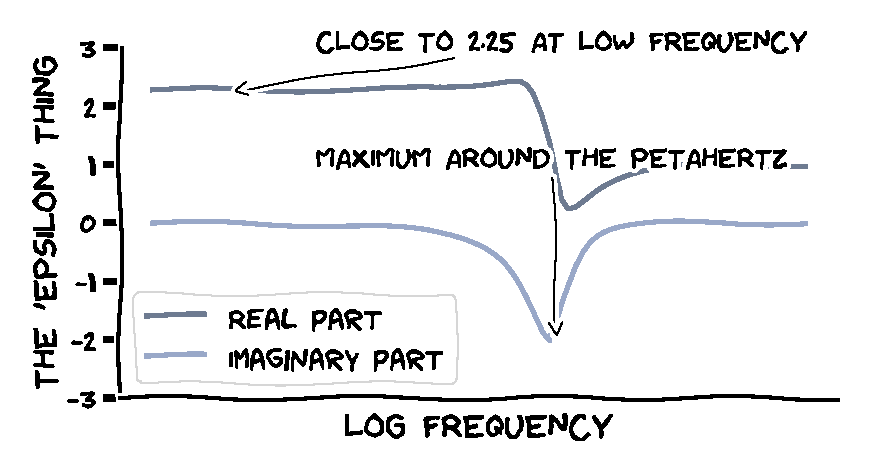
\includegraphics{figures/xkcd12.pdf}
\end{center}




% 1.3
\begin{tcolorbox}[halign=left]
  \lettrine[lines=2]{\color{ExerciseNumberColor}1.3}{}
  \emph{
    En un dieléctrico polar con dos direcciones preferentes $θ_1$ y
    $θ_2$ respecto a la dirección del campo del campo aplicado,
    obtener la polarización en términos de las poblaciones de ambos
    niveles y el campo eléctrico, que se puede considerar estacionario
    frente al tiempo de relajación.
  }
\end{tcolorbox}

Como se demostró en teoría, suponiendo una distribución de Boltzman
para las poblaciones (figura \ref{fig:populations}) se tiene
\begin{equation}
  \frac{N_1}{N_2} = e^{βpE(\cos θ_2 - \cos θ_1)}
\end{equation}

Notar que se está suponiendo un sistema de dos estados, en que $θ$
pertenece estrictamente a $\{θ_1,θ_2\}$.

\begin{marginfigure}
  \centering
  \begin{tikzpicture}
    \draw[thick, PlotDefault] (0,0) -- (3,0)
    node[black, midway, fill=white] {$N_2$}
    node [black, right] {$E_{θ_2}$};
    \draw[thick, PlotDefault] (0,-1) -- (3, -1)
    node[black, midway, fill=white] {$N_1$}
    node [black, right] {$E_{θ_1}$};
  \end{tikzpicture}
  \caption{\itshape Poblaciones para un modelo de dos estados en un dieléctrico
    con dos direcciones preferentes.}
  \label{fig:populations}
\end{marginfigure}

Sin más que despejar $p$, obtenemos
\begin{equation}
  p = \frac{\log N_1/N_2}{βE(\cos θ_2 - \cos θ_1)}
\end{equation}

% 1.4
\begin{tcolorbox}[halign=left]
  \lettrine[lines=2]{\color{ExerciseNumberColor}1.4}{}
  \emph{
    Se observa a diferentes temperaturas la parte real e imaginaria de la constante dieléctrica
    para un sólido polar con temperatura de Debye
    $Θ\sub{D}=\SI{153}{\kelvin}$. Las medidas se realizan a
    $\SI{110}{\kilo\hertz}$ y muestran un factor de pérdidas máximo a
    $\SI{270}{\kelvin}$. Demostrar que esto es consistente con la
    existencia de dos orientaciones dipolares con una barrera de
    $\SI{0.4}{\eV}$ entre ellas.
  }
\end{tcolorbox}


En primer lugar, hallamos
\footnote{
 Es trivial (pero no inmediato) utilizando
  \begin{align*}
    \Im(z) &= \frac{z - \bar{z}}{2i} \\
    \Re(z) &= \frac{z + \bar{z}}{2}
  \end{align*}
}
las partes real e imaginaria de la constante dieléctrica:
\begin{equation}
  \Re(ε) + \Im(ε) = 5 + \frac{15}{1-iωτ} = 5+ \frac{15}{1+ω^2τ^2} + 15 \frac{ωτ}{1+ω^2τ^2}
\end{equation}

El factor máximo de atenuación para la onda que atraviesa el material
se dará cuando la parte imaginaria de la constante dieléctrica sea
máxima. Como el máximo de $\frac{ζ}{1+ζ^2}$ está en $ζ=1$, se obtiene
$ω^2τ^2 = 1$, de forma que $τ=ω^{-1}$. Como se vio en teoría, la
altura de la barrera $Y=ΔU$ viene dada por
\begin{equation}
  τ = \frac{1}{ω\sub{D}} e^{βY}
\end{equation}
de forma que $ΔU = Y = β^{-1} \log \frac{ω\sub{D}}{ω}$ empleando
$τ=ω^{-1}$. Sustituyendo los \SI{270}{\kelvin} del enunciado,
$ω=2π\cdot \SI{110}{\kilo\hertz}$ y $ω\sub{D} = 2π \frac{\kb
  θ\sub{D}}{h}$, se obtiene
\begin{equation}
  ΔU = \SI{0.40}{\eV}
\end{equation}

\begin{tcolorbox}[halign=left]
  \emph{
    Representar $\Re(ε)$ y $\Im(ε)$ para el sólido a
    $\SI{110}{\kilo\hertz}$. Considerar $A=5$ y $B=15$ en la ecuación
    }

    \begin{equation*}
      ε_R + i ε_I = A + \frac{B}{1- i wt}
    \end{equation*}

    \emph{
      Deberías encontrar que $\Im(ε)$ excede el 50\% de su valor de pico
      en el rango de temperaturas entre $\SI{250}{\kelvin}$ y $\SI{290}{\kelvin}$.
    }
\end{tcolorbox}

Como puede verse en la figura, la parte imaginaria de $ε$ supera el
50\% de su valor entre $T = \SI{251}{\kelvin}$ y
$T=\SI{293}{\kelvin}$. La dependencia con $T$ la da $τ(T) = e^{βΔU}/ω\sub{D}$.

\begin{fullwidth}
  \centering
  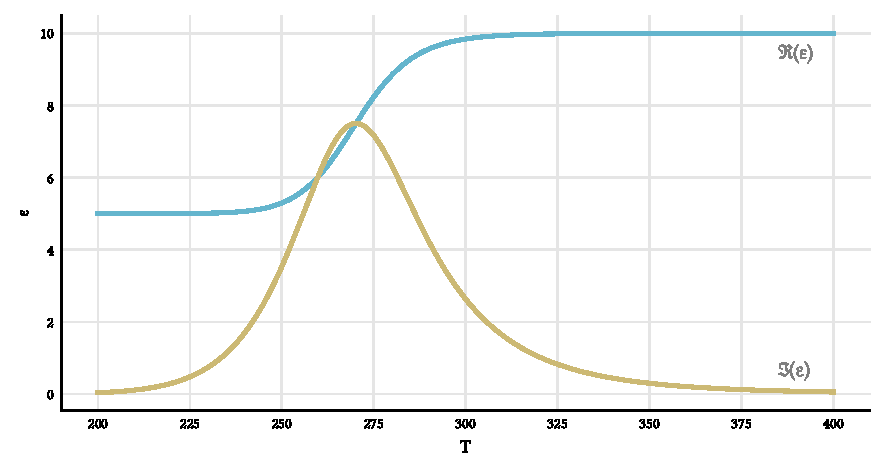
\includegraphics{figures/debye_1_4.pdf}
\end{fullwidth}

% 1.5
\begin{tcolorbox}[halign=left]
  \lettrine[lines=2]{\color{ExerciseNumberColor}1.5}{}
  \emph{Obtener las relaciones de Kramers-Kronig:}
  \begin{align*}
    χ'(ω_0)
    &= \frac{2}{π} \int_0^∞ \frac{ω χ'' \dd{ω}}{ω^2-ω_0^2} + χ'(∞) \\
    χ''
    &= - \frac{2}{π} \int_0^∞ \frac{ωχ' \dd{ω}}{ω^2-ω_0^2}
  \end{align*}
  \emph{donde $χ'(ω)$ y $χ''(ω)$ son respectivamente las partes real e
    imaginaria de la susceptibilidad.}
\end{tcolorbox}

Tomamos una función compleja analítica $f(z)$,
\marginnote{
  \begin{align*}
    f_1 &= \Re [f(z)] \\
    f_2 &= \Im [f(z)]
  \end{align*}
}
sobre la que aplicamos la \emph{integral de Cauchy}:
\begin{equation}
  \int_{-∞}^∞ \frac{f(z)}{z-z_0} \dd{z} = π i f(z) = π i (f_1 + i f_2)
  = π (if_1 - f_2)
  \label{eq:cauchyint}
\end{equation}

Además,
\begin{equation}
  \int_{-∞}^∞ \frac{f(z)}{z-z_0} \dd{z} =
  \int_{-∞}^∞ \frac{f_1}{z-z_0} \dd{z} + i\int_{-∞}^∞ \frac{f_2}{z-z_0} \dd{z}
  \label{eq:splitme}
\end{equation}

Como las ecuaciones \eqref{eq:cauchyint} y \eqref{eq:splitme}
comparten el mismo término a la izquierda, podemos igualar las partes
reales e imaginarias, obteniendo las \emph{transformadas de Hilbert}:
\begin{align}
  f_1 &= \frac{1}{π} \int_{-∞}^∞ \frac{f_2}{z-z_0} \dd{z} \label{eq:f1eq} \\
  f_2 &= \frac{-1}{π} \int_{-∞}^∞ \frac{f_1}{z-z_0} \dd{z} \label{eq:f2eq}
\end{align}

Si particularizamos para el caso $χ(ω)$ se cumple que $χ(-ω)=-χ(ω)$,
de forma que identificamos $f_1 → χ'(ω)$ y $f_2 → χ''(ω)$.

Utilizando \eqref{eq:f1eq} para $χ'(ω)$, obtenemos
\begin{equation}
  \begin{split}
    χ'(ω) &= \frac{1}{π} \int_{-∞}^∞ \frac{χ''(ω)}{ω-ω_0} \dd{ω} \\
    &= \frac{1}{π} \int_{-∞}^0 \frac{χ''(ω)}{ω-ω_0} \dd{ω}
    + \frac{1}{π} \int_0^{∞} \frac{χ''(ω)}{ω-ω_0} \\
    &= \frac{-1}{π} \int_0^∞ \frac{χ''(-ω)}{ω+ω_0} \dd{ω}
    + \frac{1}{π} \int_0^∞ \frac{χ''(ω)}{ω-ω_0} \dd{ω} \\
    &= \frac{1}{π} \int_0^∞ \frac{χ''(ω)}{ω+ω_0} \dd{ω}
    + \frac{1}{π} \int_0^∞ \frac{χ''(ω)}{ω-ω_0} \dd{ω} \\
    &= \frac{1}{π} \int_0^∞ \frac{χ''(ω)⋅(2ω+ω_0-ω_0)}{(ω+ω_0)(ω-ω_0)}
    \\
    &= \frac{2}{π} \frac{ωχ''(ω)}{ω^2-ω_0^2}
  \end{split}
\end{equation}

Q.E.D.\footnote{
  El enunciado tiene un $χ'(∞)$ extra, pero me importa entre cero y nada.
} La otra relación (parte imaginaria de la susceptibilidad) se puede
obtener procediendo igual con $χ''$ y \eqref{eq:f2eq}.

% 1.6
\begin{tcolorbox}[halign=left]
  \lettrine[lines=2]{\color{ExerciseNumberColor}1.6}{}
  \emph{
    Aplicamos un campo eléctrico en una cámara de vacío en la que se genera
    una molécula diatómica. Demostrar que la polarización electrónica
    depende del ángulo entre el eje de la molécula y la dirección del
    campo eléctrico.
  }
\end{tcolorbox}


Supongamos que los dos átomos de la molécula diatómica son idénticos,
para simplificar el análisis. Un campo externo $\symbf{E}_0$ casa una
redistribución de cargas, que a su vez crea un momento dipolar
$\symbf{p} = α_e \symbf{E}_\mathit{local}$. Esta expresión es válida
para todos los átomos, con $\symbf{E}_\mathit{local}$ escrito como
$\symbf{E}_1+\symbf{E}_2+\symbf{E}_3$ en la teoría.

En el caso de una molécula diatómica, podemos escribir el campo
$\symbf{E}_\mathit{local}$ para un átomo como la suma del externo más
el de polarización del átomo con el que forma la molécula:
\begin{equation}
  \begin{split}
    \symbf{E}_\mathit{local} &= \symbf{E}_0 + \symbf{E}_d \\
    &= \symbf{E}_0 + k α_e \symbf{E}_\mathit{local}
  \end{split}
\end{equation}

donde $k$ es una constante de proporcionalidad. Obtenemos el momento
dipolar $\symbf{p}$ de cada átomo en función de $\symbf{E}_0$:
\begin{equation}
  \symbf{p} = α_e \symbf{E}_\mathit{local} = \frac{α_e}{1-kα_e} \symbf{E}_0
\end{equation}

Para cada molécula, $\symbf{p}\sub{T} = 2 \symbf{p}$. La
polarización total del gas será
\begin{equation}
  \symbf{P} = \frac{1}{V} \frac{2α_e}{1-kα_e} \symbf{E}_0 ≃
  \frac{2α_e}{V} (1+kα_e) \symbf{E}_0
\end{equation}
para $kα_e≪1$. Notar que si $k$ es una función del ángulo $θ$
del eje de la molécula con $\symbf{E}_0$, $\symbf{P}$ también lo
será. Comprobamos si realmente $k=f(θ)$ utilizando que el campo
dipolar se puede escribir como $\symbf{E}_d = \frac{3(\symbf{p}
  \symbf{r})\symbf{r} - r^2 \symbf{p}}{4πε_0r^5}$ y que
$\symbf{p}=α_e \symbf{E}_\mathit{local}$:
\begin{equation}
  \symbf{E}_d = \frac{3α_e \symbf{E}_\mathit{local} \cos θ
    \symbf{r} - r^2 α_e \symbf{E}_\mathit{local}}{4πε_0r^5}
\end{equation}

Si $θ=0$ (molécula alineada con $\symbf{E}_0$), empleando que
$\symbf{r}=\symbf{d}∥\symbf{E}$ en dicho caso, se tiene
\begin{equation}
  \symbf{E}_d = k_∥ α_e \symbf{E}_\mathit{local}
\end{equation}
donde $k_∥ = \frac{1}{2πε_0d^3}$.

Si $θ=\nicefrac{π}{2}$ (molécula perpendicular a $\symbf{E}_0$), se
tiene
\begin{equation}
  \symbf{E}_d = k_⟂ α_e \symbf{E}_\mathit{local}
\end{equation}
donde $k_⟂ = \frac{-1}{4πε_0d^3}$.

Notamos que $\symbf{E}_d = k(θ)α_e \symbf{E}_\mathit{local}$, de
forma que $\symbf{E}_d$ depende la orientación $θ$ del dipolo, Q.E.D.

\begin{tcolorbox}[halign=left]
  \emph{
    El alineamiento completo de las moléculas se logra aplicando un
    campo eléctrico grande. Bajo esta situación, obtener como cambia
    el índice de refracción si la luz incidente está polarizada de
    forma paralela o de forma perpendicular  al eje de la molécula .
    Suponer moléculas diatómicas de longitud $d$ y con $α_e$ similar
    para cada átomo.
  }
\end{tcolorbox}
Partimos de la ecuación de Clausius-Mossoti:
\begin{equation}
  \frac{ε-1}{ε+2} = \frac{1}{3ε_0} \sum_{} N_i α_i = \frac{Nα}{3ε_0} =
  \frac{n^2 - 1}{n^2 +2}
\end{equation}
donde se ha empleado que $n^2 = ε$. Despejando $n$ y suponiendo
$\frac{Nα}{3ε_0}≪1$,
\begin{equation}
  n = \frac
    {  \sqrt{ 1+2 \frac{Nα}{3ε_0}  }  }
    {    \sqrt{   1 -\frac{Nα}{3ε_0}}  }  ≃ 1 + \frac{Nα}{2ε_0}
\end{equation}
de forma que $Δn = n_∥ - n_⟂ = \frac{N}{2ε_0}(α_∥-α_\perp)$.
Utilizando $α=2α_e(1+kα_e)$ y los valores hallados para $k_∥,k_⟂$, se
obtiene
\begin{equation}
  Δn = \frac{N}{2ε_0} (2α_e + 2k_∥α_e^2 - 2α_e + 2k_⟂α_e^2) = \frac{3Nα_e^2}{4πε_0^2d^3}
\end{equation}

\begin{tcolorbox}[halign=left]
  \emph{
    Este es el principio de las células Kerr.
  }
\end{tcolorbox}
k


% 1.7
\begin{tcolorbox}[halign=left]
  \lettrine[lines=2]{\color{ExerciseNumberColor}1.7}{}
  \emph{
    Aplicamos un voltaje oscilante con amplitud constante en los
    brazos de un condensador que contiene un dieléctrico polar con
    tiempo de relajación uniforme. Obtener una expresión para las
    pérdidas caloríficas en función de la frecuencia y demostrar que
    el valor máximo de $\Im(ε)$ se obtiene a una frecuencia en la que las
    pérdidas caloríficas son justo de la mitad de su valor máximo.
  }
\end{tcolorbox}
En el marco de la teoría de Debye, asumimos $α_i = \frac{α_0}{1-iωτ}$.
Para escribir $ε=ε_0(1+χ)$ calculamos $χ_i$ en función de las $α_i$:
\begin{equation}
  χ  = \frac{P}{ε_0 E} = \frac{1}{ε_0 E} \sum_{} N_j α_j \symbf{E}_\mathit{local}
\end{equation}
donde $α_j$ puede ser la polarizabilidad iónica ($α_i$) o la electrónica ($α_e$).
Suponiendo un campo local igual al aplicado, podemos cancelar las $E$
de numerador y denominador:
\begin{equation}
  χ = \frac{1}{ε_0} (Nα_i + Nα_e)
\end{equation}
De forma que, finalmente, obtenemos
\begin{equation}
  ε = ε_0(1+χ) = ε_0 \left( 1+\frac{Nα_0}{1-iωτ} + \frac{Nα_e}{ε_0}
  \right)
\end{equation}

Introducimos la constante dieléctrica estática $ε(0)$ y la de
frecuencias ópticas $ε(∞)$:
\begin{align}
  \frac{ε(0)}{ε_0} &= 1 + \frac{α_eN}{ε_0} + \frac{α_0N}{ε_0} \\
  \frac{ε(∞)}{ε_0} &= 1 + \frac{α_eN}{ε_0}
\end{align}
con ellas, escribimos $ε$ como suma de una parte real y una
imaginaria:
\begin{equation}
  ε = \frac{ε(∞)}{ε_0} + \frac{1}{ε_0}\frac{ε(0) -ε(∞)}{1+ω^2τ^2} \ \ + \ \ i ⋅ \frac{1}{ε_0}\frac{[ε(0) -
    ε(∞)] ωτ}{1+ω^2τ^2}
\end{equation}
La parte de interés es la imaginaria, ya que es la causa del calor
disipado, igual a $Q=ω\Im(ε)$. Vemos que su máximo ($\dv{ω}\Im(ε) =0$)
ocurre en $ω^2τ^2 =1$, de forma que la frecuencia del máximo es
$\nicefrac{1}{τ}$. Sustituyendo de vuelta en $\Im(ε)$, obtenemos
\begin{equation}
  \eval{\Im(ε)}_{\nicefrac{1}{τ}} =\frac{1}{ε_0} \frac{ε(0)-ε(∞)}{2}
\end{equation}
mientras que el calor disipado alcanza su máximo en $ω→∞$, debido al
factor $ω$ extra:
\begin{equation}
  \lim_{ω→∞} Q = \lim_{ω→∞} \frac{1}{ε_0} \frac{ω^2τ}{1+ω^2τ^2} [ε(0)-ε(∞)] =
  \frac{1}{ε_0} [ε(0)-ε(∞)]
\end{equation}

De forma que el máximo de $\Im(ε)$ vale la mitad del máximo calor
disipado, Q.E.D (figura \ref{fig:sopainful}).

\begin{tcolorbox}[halign=left]
  \emph{
    ¿Por qué este método no es idoneo para obtener la frecuencia de rejación?
  }
\end{tcolorbox}

Porque se ha supuesto que todas las medidas de disipación se han hecho
a la misma temperatura. Debido a que el sistema está disipando calor,
esto es más falso que las peleas de los power rangers.

\begin{marginfigure}
  \centering
  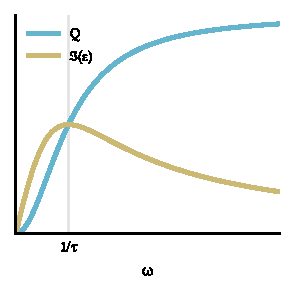
\includegraphics{figures/sopainful.pdf}
  \caption{\itshape $\Im(ε)$ alcanza como máximo $Q/2$.}
  \label{fig:sopainful}
\end{marginfigure}


% 1.8
\begin{tcolorbox}[halign=left]
  \lettrine[lines=2]{\color{ExerciseNumberColor}1.8}{}
  \emph{
    Un plasma a baja presión contiene $n$ electrones libres por unidad
    de volumen. Demostrar que la constante dieléctrica a frecuencia
    $f$ es
  }
  \begin{equation}
    ε_r = 1 - \frac{ne^2}{4π^2f^2mε_0}
  \end{equation}
  \emph{Discutir la propagación de la radiación electromagnética a
    través del plasma en función de la frecuencia.}
\end{tcolorbox}
Un electron libre bajo un campo eléctrico local
$E_\mathit{local}=E_0\sin ωt$ experimenta una fuerza $-eE_0\sinωt$.
La ecuación del movimiento queda como $m\ddot{x} = F$, con $x$ el
desplazamiento respecto a la posición de equilibrio.
Probamos con una solución $x=x_0 \sin ωt$, obteniendo
\begin{equation}
  x_0 = \frac{eE_0}{mω^2}
\end{equation}
Como el momento dipolar es $p_0=-ex_0 = \frac{-e^2E_0}{mω^2}$, se
tiene una susceptibilidad
\begin{equation}
  χ = \frac{P}{ε_0E_0} = \frac{-ne^2 E_0}{mω^2}\frac{1}{ε_0E_0} = \frac{-ne^2}{ε_0mω^2}
\end{equation}
donde se ha empleado $P=np_0$. Empleando $ε_r = χ+1$ y $ω=2πf$,
obtenemos la expresión del enunciado.

Vemos que para frecuencias muy bajas $ε_r$ es negativa y la radiación se
absorbe ($n$ imaginaria). Para frecuencias muy altas, $ε=1$ y el plasma
transparente a la radiación.
\begin{tcolorbox}[halign=left]
  \emph{
    Un metal experimenta un efecto similar por ser equiparable a un
    gas de electrones; aplicar los resultados previos al caso del
    sodio y comparar la frecuencia del valor crítico $ε\sub{R}=0$ con
    las observaciones experimentales.
  }
\end{tcolorbox}
Se emplean los
datos del sodio\footnote{
  $\SI{22.9}{\gram\per\mole}$ y $ρ=\SI{968}{\kilo\gram\per\cubic\metre}$
}, obteniendo $ε=0 → f=\SI{1.43e15}{\per\second}$, que equivale a
$\SI{2097.9}{\angstrom}$.

No hablo con experimentales.

\chapter*{Tema 2}
% 2.1
\begin{tcolorbox}[halign=left]
  \lettrine[lines=2]{\color{blue!50!white}2.1}{}
  \emph{Applying Hund's rules, obtain the lowest-lying J-multiplet for
    ions in a solid for the case of 1 to 9 electron occupancy in a \emph{d}
    shell ($ℓ=2$) and 1 to 13 electrons in a \emph{f} shell ($ℓ=3$).
    Use spectroscopic notation to give those states.
    }
\end{tcolorbox}
\marginnote{
  \begin{center}
    
\includegraphics[width=2cm]{figures/flag.pdf}
  \end{center}
}

Each one of Hund's rules gives us a restriction in the spectroscopic
term of the lowest lying J-multiplet.

\begin{flushright}
\textit{Hund's Rules}
\end{flushright}

\begin{flushleft}
  \textsc{First Hund's Rule:}
  \emph{
    For a given electron configuration, the term with maximum
    multiplicity has the lowest energy. The multiplicity is equal to $2S +
    1$, where $S = \sum_{i} S_i$ is the total spin angular momentum for
    all electrons.
  }
\end{flushleft}

This rule implies that we must place the greatest amount possible of
electrons in the ``empty boxes'' (different values of $\ell_z$) of the
orbital without any partner.

For example, in a \emph{p} orbital (three boxes), is preferable to have
the configuration {\orbital{↓}\orbitalsep\orbital{↓}\orbitalsep\orbital{ }} than the configuration
{\orbital{↓↑}\orbitalsep\orbital{ }\orbitalsep\orbital{ }}.

\begin{flushleft}
  \textsc{Second Hund's Rule:}
  \emph{
    For a given multiplicity, the term with the largest value of the total
    orbital angular momentum quantum number $L$ has
    the lowest energy.
  }
\end{flushleft}

This means that we have to fill the boxes starting by the ones with
the greatest $\ell_z$.

\begin{flushleft}
  \textsc{Third Hund's Rule:}
  \emph{
    For a given term, in an atom with outermost subshell half-filled
    or less, the level with the lowest value of the total angular momentum
    quantum number $J$ (where $\symbf{J} = \symbf{L} + \symbf{S}$) lies
    lowest in energy. If the subshell is more than half-filled, then
    the lowest-lying level is the one with the greatest $J$.
  }
\end{flushleft}

Once $S = \sum_{i} S_i$ (with $S_i ∈ \pm \oh$) and $L = \sum_{i} \ell_z$
are computed, $J = \abs{L \pm S}$, since $J = L ⊗ S = \{L+S , ⋯,
\abs{L-S}\}$ in jumps of 1. If the subshell is half-filled or less, we
choose $J = \abs{L-S}$, else we take $J = \abs{L+S}$.

\begin{flushright}
d \textit{subshell}
\end{flushright}

To find the spectroscopic terms of each ground state configuration
(with $n$ electrons each), we fill the orbitals from the highest
$\ell_z$ to the lowest, trying to keep the maximum possible number of
unpaired electrons.

\begin{center}
  \begin{tabular}[center]{l|lccccc|c|c|c|c}
    $n$ & $\ell_z=$ & $2$  & $1$  & $0$  & $-1$ & $-2$ & $S=\sum_{}s$      & $L = \sum_{} \ell_z$ & J                 &                                                 \\ \hline
    1   &           & {↓}  & {}   & {}   & {}   & {}   & $\nicefrac{1}{2}$ & $2$                  & $\nicefrac{3}{2}$ & \isotope[2]{D}\textsubscript{$\nicefrac{3}{2}$} \\
    2   &           & {↓}  & {↓}  & {}   & {}   & {}   & $1              $ & $3$                  & $2              $ & \isotope[3]{F}\textsubscript{$2              $} \\
    3   &           & {↓}  & {↓}  & {↓}  & {}   & {}   & $\nicefrac{3}{2}$ & $3$                  & $\nicefrac{3}{2}$ & \isotope[4]{F}\textsubscript{$\nicefrac{3}{2}$} \\
    4   &           & {↓}  & {↓}  & {↓}  & {↓}  & {}   & $2              $ & $2$                  & $0              $ & \isotope[5]{D}\textsubscript{$0              $} \\
    5   &           & {↓}  & {↓}  & {↓}  & {↓}  & {↓}  & $\nicefrac{5}{2}$ & $0$                  & $\nicefrac{5}{2}$ & \isotope[6]{S}\textsubscript{$\nicefrac{5}{2}$} \\
    6   &           & {↓↑} & {↓}  & {↓}  & {↓}  & {↓}  & $2              $ & $2$                  & $4              $ & \isotope[5]{D}\textsubscript{$4              $} \\
    7   &           & {↓↑} & {↓↑} & {↓}  & {↓}  & {↓}  & $\nicefrac{3}{2}$ & $3$                  & $\nicefrac{9}{2}$ & \isotope[4]{F}\textsubscript{$\nicefrac{9}{2}$} \\
    8   &           & {↓↑} & {↓↑} & {↓↑} & {↓}  & {↓}  & $1              $ & $3$                  & $4              $ & \isotope[3]{F}\textsubscript{$4              $} \\
    9   &           & {↓↑} & {↓↑} & {↓↑} & {↓↑} & {↓}  & $\nicefrac{1}{2}$ & $2$                  & $\nicefrac{5}{2}$ & \isotope[2]{D}\textsubscript{$\nicefrac{5}{2}$} \\
    10  &           & {↓↑} & {↓↑} & {↓↑} & {↓↑} & {↓↑} & $0              $ & $0$                  & $0              $ & \isotope[1]{S}\textsubscript{$0              $} \\
  \end{tabular}
\end{center}

Notice how until $n=5$ included we have $J = \abs{L-S}$ (the subshell
is half-filled or less) and from there $J = \abs{L+S}$.

The case $n=10$ (complete subshell) has been included for completeness.


\begin{flushright}
f \textit{subshell}
\end{flushright}

The process is completely identical to the one shown when solving
the \emph{d} subshell, but now there is room for 14 electrons and 7
possible $\ell_z$ values.

\begin{center}
  \begin{tabular}[center]{l|lccccccc|c|c|c|c}
    $n$ & $\ell_z=$ & $3$  & $2$  & $1$  & $0$  & $-1$ & $-2$ & $-3$ & $S=\sum_{}s$      & $L = \sum_{} \ell_z$ & J                   &                                                   \\ \hline
    1   &           & {↓}  & { }  & { }  & { }  & { }  & { }  & { }  & $\nicefrac{1}{2}$ & $3$                  & $\nicefrac{5}{2}  $ & \isotope[2]{F}\textsubscript{$\nicefrac{5}{2}  $} \\
    2   &           & {↓}  & {↓}  & { }  & { }  & { }  & { }  & { }  & $1              $ & $5$                  & $4                $ & \isotope[3]{H}\textsubscript{$4                $} \\
    3   &           & {↓}  & {↓}  & {↓}  & { }  & { }  & { }  & { }  & $\nicefrac{3}{2}$ & $6$                  & $\nicefrac{9}{2}  $ & \isotope[4]{I}\textsubscript{$\nicefrac{9}{2}  $} \\
    4   &           & {↓}  & {↓}  & {↓}  & {↓}  & { }  & { }  & { }  & $2              $ & $6$                  & $4                $ & \isotope[5]{I}\textsubscript{$4                $} \\
    5   &           & {↓}  & {↓}  & {↓}  & {↓}  & {↓}  & { }  & { }  & $\nicefrac{5}{2}$ & $5$                  & $\nicefrac{5}{2}  $ & \isotope[6]{H}\textsubscript{$\nicefrac{5}{2}  $} \\
    6   &           & {↓}  & {↓}  & {↓}  & {↓}  & {↓}  & {↓}  & { }  & $2              $ & $3$                  & $0                $ & \isotope[7]{F}\textsubscript{$0                $} \\
    7   &           & {↓}  & {↓}  & {↓}  & {↓}  & {↓}  & {↓}  & {↓}  & $\nicefrac{7}{2}$ & $0$                  & $\nicefrac{7}{2}  $ & \isotope[8]{S}\textsubscript{$\nicefrac{7}{2}  $} \\
    8   &           & {↓↑} & {↓}  & {↓}  & {↓}  & {↓}  & {↓}  & {↓}  & $3              $ & $3$                  & $6                $ & \isotope[7]{F}\textsubscript{$6                $} \\
    9   &           & {↓↑} & {↓↑} & {↓}  & {↓}  & {↓}  & {↓}  & {↓}  & $\nicefrac{5}{2}$ & $5$                  & $\nicefrac{15}{2} $ & \isotope[6]{H}\textsubscript{$\nicefrac{15}{2} $} \\
    10  &           & {↓↑} & {↓↑} & {↓↑} & {↓}  & {↓}  & {↓}  & {↓}  & $2              $ & $6$                  & $8                $ & \isotope[5]{I}\textsubscript{$8                $} \\
    11  &           & {↓↑} & {↓↑} & {↓↑} & {↓↑} & {↓}  & {↓}  & {↓}  & $\nicefrac{3}{2}$ & $6$                  & $\nicefrac{15}{2} $ & \isotope[4]{I}\textsubscript{$\nicefrac{15}{2} $} \\
    12  &           & {↓↑} & {↓↑} & {↓↑} & {↓↑} & {↓↑} & {↓}  & {↓}  & $1              $ & $5$                  & $6                $ & \isotope[3]{H}\textsubscript{$6                $} \\
    13  &           & {↓↑} & {↓↑} & {↓↑} & {↓↑} & {↓↑} & {↓↑} & {↓}  & $\nicefrac{1}{2}$ & $3$                  & $\nicefrac{7}{2}  $ & \isotope[2]{F}\textsubscript{$\nicefrac{7}{2}  $} \\
    14  &           & {↓↑} & {↓↑} & {↓↑} & {↓↑} & {↓↑} & {↓↑} & {↓↑} & $0              $ & $0$                  & $0                $ & \isotope[1]{S}\textsubscript{$0                $} \\
  \end{tabular}
\end{center}

This time $J = \abs{L-S}$ was used until $n=6$ included, from there $J = \abs{L+S}$ was employed.


% 2.2
\begin{tcolorbox}[halign=left]
  \lettrine[lines=2]{\color{ExerciseNumberColor}2.2}{}
  \emph{Demonstrate that the magnetization of a set of atoms or ions with identical angular momentum $J$ is proportional to the Brillouin function:}
  \begin{equation*}
    \text{B}_J(x)=\frac{2J+1}{2J}\coth \left( \frac{2J+1}{2J}x \right)-\frac{1}{2J}\coth\left( \frac{1}{2J}x \right)
  \end{equation*}
\end{tcolorbox}

Según la física estadística, la magnetización de un sistema se puede
escribir, usando la esatadística de Boltzmann, como:

\begin{equation}
M=\frac{\sum_J m_Je^{-E_J\beta}}{\sum_J e^{-E_J\beta}}
\end{equation}

donde $Z ≔ \sum_J e^{-E_J\beta}$ es la función de partición.
La energía de un microestado viene dada por:

\begin{equation}
E_J=m_J g \mu_B\abs{\vec{B}}
\end{equation}

donde $m_J \in \left[ -J,J \right]$ es la tercera componente del
momento angular mangético total. Por tanto, $m_J$ toma $2N+1$ valores
enteros. Realizando el cambio de variable $x=gJ_{\mu_B}\beta$, la
magnetización se puede escribir como:

\begin{equation}
M=\frac{\displaystyle \sum_{m_J=-J}^{J}m_Je^{-xm/J}}{\displaystyle\sum_{m_J=-J}^{J}e^{-xm/J}}
\end{equation}

Se puede demostrar que
$\frac{\partial}{\partial x}\sum_{m_J} e^{-xm/J}=-\sum_{m_J}
\frac{m}{J} e^{-xm/J}$. Esto permite escribir la magnetización como
proporcional a la derivada del logaritmo de la función de partición:

\begin{equation}
M\propto\frac{\partial \ln Z}{\partial x}
\label{eq:2.2_log}
\end{equation}

%pls kill me

Por tanto, operando para obtener $Z$ explíticitamente:

\begin{align*}
Z&=\sum^J_{m_J=-J}e^{-xm/J}=e^{-\left( -\frac{x}{J}\right)J}\sum^{2J+1}_{m_J=0}e^{-xm/J}=
e^x\frac{1-e^{-x\left( 2J+1 \right)/J}}{1-e^{-x/J}}\\
&=\frac{e^x-e^{-x\left( 2+1/J -1\right)}}{1-e^{-x/J}}=\frac{e^x-e^{-x\left( J+1\right)/J}}{1-e^{-x/J}}=\frac{e^{-x/2J}}{e^{-x/2J}}\frac{e^{x(1+1/2J)}-e^{-x[(J+1)/J-1/2J]}}{e^{x/2J}-e^{-x/2J}}\\
&=\frac{e^{x(1+1/2J)}-e^{-x[(J+1)/J-1/2J]}}{e^{x/2J}-e^{-x/2J}}=\frac{e^{x(2J+1)/2J}-e^{-x(2J+1)/2J}}{e^{x/2J}-e^{-x/2J}}\\
&=\frac{2\sinh\left( \frac{(2J+1)x}{2J} \right)}{2\sinh \left(\frac{x}{2J}\right)}
\end{align*}

donde se han usado las propiedades de la serie geométrica. Definiendo
$\alpha=(2J+1)/2J$ y $\gamma=1/2J$ y sustituyendo en
\eqref{eq:2.2_log}:

\begin{align*}
M&\propto \frac{\partial\ln Z}{\partial x}=\frac{\alpha\cosh(\alpha x)\sinh(\beta x)-\beta\sinh(\alpha x)\cosh(\beta x)}{\sinh^2(\beta x)}\left(\frac{\sinh(\alpha x)}{\sinh(\beta x)}\right)^{-1}\\
&=\alpha \coth(\alpha x)-\beta \coth(\beta x)\\
&=\left( \frac{2J+1}{2J}x \right) \coth \left(\frac{2J+1 x}{2J}\right)-\left( \frac{1}{2J}\right) \coth\left( \frac{x}{2J} \right)
\end{align*}

Q.E.D.

\begin{tcolorbox}[halign=left]
  \lettrine[lines=2]{\color{ExerciseNumberColor}2.3}{}
  \emph{El teorema de Wigner-Eckart establece que los elementos de
    matriz de cualquier operador vectorial en el espacio de $2J+1$
    dimensiones de autoestados de $J^2$ y $J_z$ para un valor dado de
    $J$ es proporcional a los elementos de matriz de $\symbf{J}$:}
  \begin{equation*}
    \mel{JLSJ_z}{\symbf{L}+g_0 \symbf{S}}{JLSJ_z} = g(JLS)
\mel{JLSJ_z}{\symbf{J}}{JLSJ_z}
  \end{equation*}
  donde $g$ es el factor de Landé. Demostrar que
  \begin{equation*}
    g(JLS)  = \frac{1}{2}(g_0+1) - \frac{1}{2} (g_0 -1) \frac{L(L+1) -
    S(S+1)}{J(J+1)}
  \end{equation*}
\end{tcolorbox}

El teorema de la proyección establece que
\begin{equation}
  \expval{\symbf{A}} = \frac{\expval{\symbf{A} ⋅
      \symbf{J}}}{\expval{J^2}} \expval{\symbf{J}}
\end{equation}
Si tomamos $\symbf{A} = \symbf{L} + g_0 \symbf{S}$ y lo aplicamos a
la primera expresión del enunciado, obtenemos
\begin{equation}
  \expval{\symbf{L}+ g_0 \symbf{S}} =
  \frac{\expval{(\symbf{L})⋅\symbf{J}}}{\expval{J^2}}
  \expval{\symbf{J}}
  +
  \frac{\expval{(g_0\symbf{S})⋅\symbf{J}}}{\expval{J^2}}
  \expval{\symbf{J}}
  = g(JLS) \expval{\symbf{J}}
\end{equation}
de forma que
\begin{equation}
  g(JLS) =
  \frac{\expval{\symbf{L}⋅\symbf{J}}}{\expval{J^2}}
  +
  g_0\frac{\expval{\symbf{S}⋅\symbf{J}}}{\expval{J^2}}
\end{equation}
Para obtener los valores medios de $\symbf{L}⋅\symbf{J}$ y
$\symbf{S}⋅\symbf{J}$ los reescribimos en términos de $J^2,L^2$ y $S^2$:
\marginnote{$\symbf{J} = \symbf{L} + \symbf{S}$}
\begin{align}
  S^2 &= (\symbf{J}-\symbf{L})^2 = J^2 + L^2 - 2 \symbf{J} ⋅
        \symbf{L} \ \rightarrow \ \symbf{J}⋅\symbf{L} =
        \frac{J^2+L^2-S^2}{2} \\
  L^2 &= (\symbf{J}-\symbf{S})^2 = J^2 + S^2 - 2 \symbf{J} ⋅
  \symbf{S} \ \rightarrow \ \symbf{J}⋅ \symbf{S} = \frac{J^2+S^2-L^2}{2}
\end{align}
En unidades de $ℏ^2$, los valores medios son
\begin{align}
  \expval{\symbf{L}⋅\symbf{J}} &= \expval{\symbf{J}⋅\symbf{L}} = ⋯ = \frac{J(J+1) + L(L+1) - S(S+1)}{2} \\
  \expval{ \symbf{S} ⋅ \symbf{J}} &= \expval{ \symbf{J} ⋅
                                      \symbf{S}} = ⋯ = \frac{J(J+1) + S(S+1) -L(L+1)}{2}
\end{align}
sin más que sustituir en los resultados anteriores los valores de los
$\expval{ζ^2}=ζ(ζ+1)$ con $ζ$ igual a $J$, $L$ o $S$. Sustituyendo en
la expresión de $g(JLS)$ y simplificando, obtenemos el resultado del enunciado.

Notamos varias cosas interesantes\footnote{\verb~</s>~}:
\begin{itemize}
\item Para un electron libre se tiene $L=0, S=J=\oh$ y se recupera
  $g(JLS)=g_0$. Conocemos, de la ecuación de Dirac, que $g_0=2$.
\item En el caso más general habría que considerar el operador
  $g\sub{L} \symbf{L} + g_0 \symbf{S}$, con $g\sub{L}$ dando cuenta
  del acoplamiento entre el campo magnético y el momento angular
  orbital. En el caso del enunciado, $g\sub{L}=1$, muy usual y válido
  para protones y electrones. Para neutrones, que no poseen momento
  magnético orbital por no estar cargados, $g\sub{L}=0$.
\end{itemize}


% 2.4
\begin{tcolorbox}[halign=left]
  \lettrine[lines=2]{\color{blue!50!white}2.4}{}
  \emph{Las funciones propias de un electrón libre 3D con degeneración
    $S$ vienen dadas por}
  \begin{equation*}
    \begin{split}
      Ψ_1 &= xz ⋅ f(r) \\
      Ψ_2 &= yz ⋅f(r) \\
      Ψ_3 &= xy⋅ f(r) \\
      Ψ_4 &= (x^2-y^2)⋅ f(r) \\
      Ψ_5 &= (3z^2-1)⋅ f(r) \\
    \end{split}
  \end{equation*}
  \emph{Obtener el splitting del estado fundamental degenerado cuando
    el electrón está bajo un campo eléctrico de simetría rómbica:}
  \begin{equation*}
    V = Ax^2 + By^2 + Cz^2
  \end{equation*}
  \emph{Demostrar el quenching del momento orbital. Discutir
    utilizando los resultados previos el caso con simetría tetragonal ($A=B$). }
\end{tcolorbox}

Estudiamos como cambian los niveles de energía al aplicar un $V=Ax^2 +
By^2 + Cz^2$, quedando el hamiltoniano como $ \Ham = \Ham_0 + V$. Sus
elementos de matriz, que corresponden a los $ΔE$, serán
\begin{equation}
  \Ham_{ij} = \mel{ψ_i}{V}{ψ_j} = \Ham_{ji}
\end{equation}
Muchos elementos son nulos por estar integrándose funciones impares en
$\mathbb{R}^3$. Esto ocurre para todos los términos
\textit{off-diagonal} excepto el $\Ham_{4,5}$, de forma que la matriz
será diagonal excepto por un bloque 2×2 en las filas y columnas 4 y 5.
\marginnote{$\Ham ∼ \mqty(\dmat{○,○,○,○,    ○&○\\○&○})$}


Las integrales que se obtienen en los $\Ham_{ij}$ se pueden resumir en
tres tipos:

\begin{align}
  S_1 &= \iiint \abs{f(r)}^2 x^4z^2 \dd{V} = ⋯ =
        \frac{4π}{35} \int_0^∞ \abs{f(r)}^2 r^8 \dd{r} \\
  S_2 &= \iiint \abs{f(r)}^2 x^2 y^2 \dd{V} = ⋯ =
        \frac{4π}{15} \int_0^∞ \abs{f(r)}^2 r^6 \dd{r}\\
  S_3 &= \iiint \abs{f(r)}^2 z^2 \dd{V}= ⋯ =
        \frac{4π}{3} \int_0^∞ \abs{f(r)}^2 r^4 \dd{r}
\end{align}
donde se han pasado $x, y, z$ a coordenadas esféricas\footnote{
  \begin{align*}
    x &= r \sin θ \cos φ \\
    y &= r \sin θ \sin φ \\
    z &= r \cos θ \\
    \dd{V} &= r^2 \sin θ \ \dd{r} \dd{θ} \dd{φ}
  \end{align*}
} para llegar a integrales que sólo dependan de $r$.

Con ellas podemos expresar de forma concisa los elementos de matriz,
notando que
\begin{align}
  \iiint \abs{f(r)}^2 x^2 y^2 z^2 \dd{V} &= ⋯ =
                                           \frac{4π}{105}\int_0^∞
                                           \abs{f(r)}^2 r^8 \dd{r}=
                                           \nicefrac{1}{3} S_1 \\
  \iiint \abs{f(r)}^2 x^6 \dd{V} &=
                                   ⋯ =
                                   \frac{4π}{7}\int_0^∞
                                   \abs{f(r)}^2 r^8 \dd{r}
                                   = 5 S_1
\end{align}
pasando de nuevo a coordenadas esféricas. Expresemos los términos de
la diagonal, el procedimiento el el mismo para todos: expandir la
integral de $\mel{Ψ_i}{V}{Ψ_j}$y ponerla en función de las $S_i$.

\begin{align}
  \Ham_{11} &= \iiint \abs{f(r)}^2 x^2 z^2 (Ax^2 - By^2 + Cz^2) \dd{V}
              = (A+\nicefrac{1}{3}B + C) S_1 \\
  \Ham_{22} &= ⋯ = (\nicefrac{1}{3}A+B+C)S_1 \\
  \Ham_{33} &= ⋯ = (A+B+\nicefrac{1}{3}C)S_1 \\
  \Ham_{44} &= ⋯ = (A+B+\nicefrac{1}{3}C)4S_1 \\
  \Ham_{55} &= ⋯ = 9(A+B+5C)S_1 - 6(A+B+3C)S_2 + (A+B+C)S_3
\end{align}

falta por calcular el $\Ham_{45}$, el único fuera de la diagonal. Se obtiene
\begin{equation}
  \Ham_{45} = 2(A-B)(S_1-S_2)
\end{equation}

Para ver los niveles energéticos en este campo, calculamos los
autovalores de la matriz. Se tienen tres autovalores triviales
($\Ham_{11}, \Ham_{22}, \Ham_{33}$) por los
términos diagonales, y dos no triviales tras diagonalizar la caja 2×2:

\begin{equation}
  \mqty| \Ham_{44} -λ& \Ham_{45} \\ \Ham_{45} & \Ham_{55} - λ | =
  (\Ham_{44} - λ)(\Ham_{55}-λ) - \Ham_{45}^2 = 0
\end{equation}
obteniendo
\begin{align}
  ΔE_4 &= \frac{\Ham_{44} + \Ham_{55} + \sqrt{(\Ham_{44} - \Ham_{55})^2
  + 4 \Ham_{45}^2} }  { 2  }\\
  ΔE_5 &= \frac{\Ham_{44} + \Ham_{55} - \sqrt{(\Ham_{44} - \Ham_{55})^2
  + 4 \Ham_{45}^2} }  { 2  }
\end{align}

Notamos que los $ΔE_i$ son diferentes, lo que indica que el estado
fundamental se desdobla en 5 singletes.

% Wed Mar 22 09:03:44 CET 2017

En el caso del campo tetragonal, $A=B$ y se obtiene una matriz
puramente diagonal

\begin{align}
  \Ham_{11} &= \left( \frac{4}{3} A + C \right)S_1 \\
  \Ham_{22} &= \left( \frac{4}{3} A + C \right)S_1 \\
  \Ham_{33} &= \left( 2 A + ⅓C \right)S_1 \\
  \Ham_{44} &= 4\left( 2 A + ⅓C \right)S_1 \\
  \Ham_{55} &= 9\left( 2 A + 5C \right)S_1 - 6 (2A+3C)S_2 + (2A+C)S_3 \\
  \Ham_{45} &= \Ham_{54} = 0
\end{align}

Vemos que ahora solo hay tres $ΔE_i$ únicos; se forman dos dobletes y
un singlete.

Para estudiar si hay \textit{quenching} orbital, calculamos el valor
de $\expval{L_z}=\expval{ - i ℏ \pdv{φ}}$, si se anula habrá \textit{quenching}.

Para cada orbital $\mel{Ψ_i}{L_z}{Ψ_i}$ obtenemos un puro de cuidado,
pero como las integrales no se hacen, se huelen\footnote[][-1.5cm]{
    
\includegraphics[width=0.15\textwidth]{figures/joke.png}
}, con paciencia vemos
que se anulan. Por lo tanto, hay quenching orbital para ambos
potenciales del problema.


% 2.5
\begin{tcolorbox}[halign=left]
  \lettrine[lines=2]{\color{blue!50!white}2.5}{}
  \emph{Un sistema paramagnético de $N$ átomos por unidad de volumen
    con $L=0$ y $S=\oh$ tiene diferentes poblaciones para sus niveles
    a temperatura $T$, que se han dividido bajo un campo magnético.
    Obtener la población de los niveles y la magnetización suponiendo
    $N=\SI{1e22}{\per\cubic\centi\metre}$, $H=\SI{25}{\kilo\oersterd}$
    y $T∈\{\SI{300}{\kelvin}, \SI{4}{\kelvin}\}$.}
\end{tcolorbox}
\begin{margintable}
  In case you are still living in 1930:

  \vspace{0.55cm}

  \begin{tabular}[center]{rccr}
    \toprule
    Unidad & CGS & SI & Conversión\\
    \midrule
    $H$    & \SI{}{Oe} & \SI{}{\ampere\per\metre} & $\SI{1}{\oersterd}
                                                    = \frac{1000}{4π}\SI{}{\ampere\per\metre} $ \\
    $B$    &  \SI{}{\gauss}   &  \SI{}{\tesla} & $\SI{1}{\gauss} = \SI{1e-4}{\tesla}$  \\
    \bottomrule
  \end{tabular}
\end{margintable}

El momento magnético de un átomo libre es
$\symbf{μ} = -gμ_0 \symbf{J}$, de $J=L+S=0+\oh = \oh$ deducimos que
$m\sub{J}= \{J,J-1,\ldots,-J\} = ±\oh$. Por lo tanto,
\begin{equation}
  U = - \symbf{μ} \symbf{B} ∈ ±g \mb B = ± \mb B
\end{equation}
empleando los posibles valores de $J$ y $g=1  + \frac{J(J+1) + S(S+1)
  - L(L+1)}{2J(J+1)}= 2$. Tenemos dos niveles energéticos, separados
una distancia $2\mb B$.
\marginnote{$\mb = \SI{9.27e-24}{\joule\per\tesla}$}. Hallamos el
campo $B$ como
\begin{equation}
  B = μ_0 H =
  \underbrace{4π\SI{1e-7}{\newton\per\ampere\squared}}_{μ_0}
  \underbrace{\SI{25}{\kilo\oersterd} ⋅ \frac{1000}{4π}
    \frac{\mathrm{A\ m^{-1}}}{\mathrm{Oe}} }_{H} = \SI{2.5}{\tesla}
\end{equation}
de forma que $U ∈ ± \SI{2.32e-23}{\joule}$ sin más que sustituir el
valor de $\mb$. Obtenemos las poblaciones suponiendo una estadística
de Boltzmann:
\begin{align}
  \frac{N_{+\oh}}{N} &= \frac{e^{-βU_{+\oh}}}{e^{-βU_{+\oh}} +
                       e^{-βU_{\moh}}} \\
  \frac{N_{-\oh}}{N} &= \frac{e^{-βU_{-\oh}}}{e^{-βU_{+\oh}} +
                       e^{-βU_{\moh}}}
\end{align}
Sustituyendo las temperaturas propuestas, se obtiene
\begin{center}
  \begin{tabular}{lcc}
    \toprule
    T & $N_{+\oh}$& $N_{\moh}$ \\
    \midrule
    \SI{300}{\kelvin} & \SI{4.97e27}{\per\cubic\metre}&
                                                        \SI{5.03e27}{\per\cubic\metre} \\
    \SI{4}{\kelvin} & \SI{3.03e27}{\per\cubic\metre}&
                                                        \SI{6.97e27}{\per\cubic\metre} \\
    \bottomrule
  \end{tabular}
\end{center}
 A temperaturas altas las poblaciones están más equilibradas que a
 temperatura baja, donde la población de menor energía predomina.
 Conocidas las poblaciones hallamos la magnetización como
 \begin{equation}
 M = ΔN ⋅ μ (N_{\moh} - N_{+\oh}) \underbrace{g}_{2} \mb
\underbrace{S}_{\oh} = (N_{\moh} -N_{+\oh})\mb
 \end{equation}
 hallando $M=
 \SI{556}{\joule\per\tesla\per\cubic\metre}$ a \SI{300}{\kelvin} y
 $\SI{36253}{\joule\per\tesla\per\cubic\metre}$ a \SI{4}{\kelvin}. El
 desequilibrio de las poblaciones a \SI{4}{\kelvin} crea una
 magnetización notablemente mayor.

% 2.6
\begin{tcolorbox}[halign=left]
  \lettrine[lines=2]{\color{blue!50!white}2.6}{}
  \emph{Demostrar que el diamagnetismo no se puede explicar mediante
    física clásica. Utiliza la integral de la función de partición y
    obtenen un valor nulo para la susceptibilidad orbital del gas de electrones.}
\end{tcolorbox}
\marginnote{A este resultado se le denota \emph{teorema de Bohr y Van-Leuven}.}

Para simplificar los cálculos, supongamos un $\symbf{B} = B_0
\hat{z}$, de forma que $\symbf{A}$ es simplemente $\frac{1}{2}
\symbf{B} × \symbf{r} = \oh B (-y, x, 0)^{\mathit{T}}$.
Utilizamos el modelo de Drude para tratar el metal como un gas de
electrones no interactuantes, de hamiltoniano descomponible:
\begin{equation}
  \Ham = \sum_{j=1}^N \left[  \symbf{p}_j + \frac{e}{c}
    \symbf{A}(\symbf{r}) \right] = \sum_{j} \Ham_j
\end{equation}

El momento magnético total en el eje $\hat{z}$ es $μ_z =
\sum_{j}μ_{jz}$. En el espacio $V$ tenemos
\begin{equation}
  \begin{split}
    \expval{μ_z} &= \frac{1}{V} \frac{\iint \dd{\symbf{r}_j} \dd{\symbf{p}_j} μ_z e^{-β \Ham}
    }{\iint \dd{\symbf{r}_j} \dd{\symbf{p}_j} e^{-β \Ham}} \\
    &= \frac{1}{V} \frac{\prod_j \iint \dd{\symbf{r}_j}
      \dd{\symbf{p}_j} \sum_i μ_{iz} e^{-β \Ham_j}}
    {\prod_j \iint \dd{\symbf{r}_j} \dd{\symbf{p}_j} e^{-β \Ham_j} }
  \end{split}
\end{equation}
donde se ha empleado que $\exp(β \Ham) = \exp(β \sum_{j} \Ham_j) =
\prod_j \exp(β \Ham_j)$. Empleando que $μ_{jz}= \frac{-e}{2cB}
\symbf{v}_j \symbf{A}$,
\begin{equation}
  \expval{μ_z} ∝ \prod_j \int \dd{\symbf{p}_j} \symbf{v}_j \symbf{A}
  e^{-β \Ham_j}
\end{equation}
Por otro lado, $\dot{\symbf{r}_i} = \symbf{v}_i = -
\pdv{\Ham}{\symbf{p}_i} ∝ - \symbf{p}_i$, de forma que
\begin{equation}
  \expval{μ_z} ∝ \int \prod_j \dd{\symbf{p}_j} \ \symbf{p}_j e^{-β \Ham_j}
\end{equation}
Notamos que el hamiltoniano, función par en $\symbf{p}_j$, está
multiplicado por $\symbf{p}_j$, función impar. Por lo tanto, la
integral se anula y no existe momento magnético promedio permanente,
Q.E.D.

% 2.7
\begin{tcolorbox}[halign=left]
  \lettrine[lines=2]{\color{blue!50!white}2.7}{}
  \emph{El ion Cu\textsuperscript{2+} está en el centro de un octaedro
    de seis moléculas de H\textsubscript{2}O. Debido a su influencia
    los orbitales del estado fundamental sufren splitting por el campo
    cristalino, como muestra la figura. Obtener la contribución
    anisotrópica al factor de Landé en función de la constante $λ$ de
    acoplo espín-órbita.}
  \begin{center}
    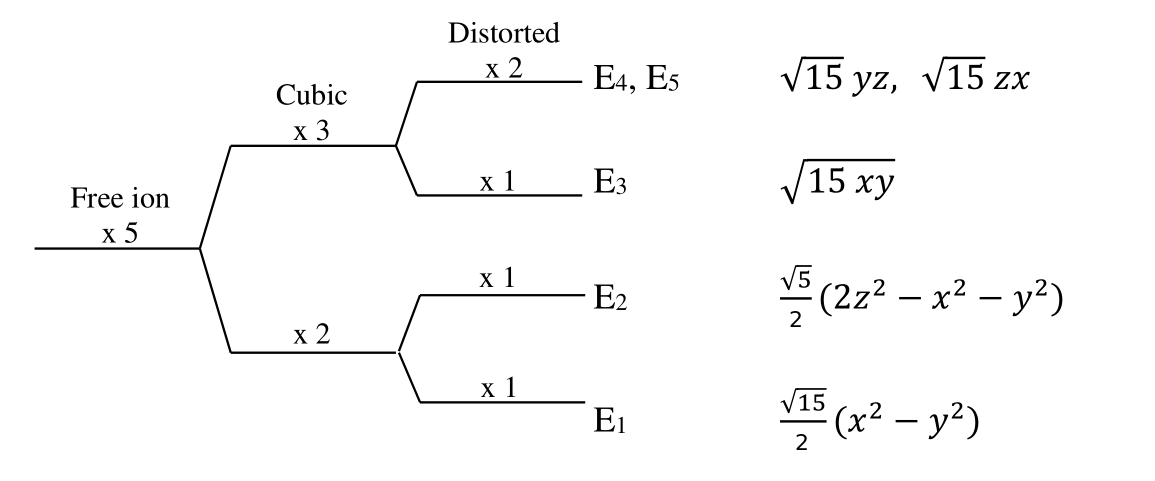
\includegraphics[width=\textwidth]{figures/figure2-7.png}
  \end{center}
\end{tcolorbox}
\marginnote[-3cm]{En el enunciado original, en lugar de $\frac{1}{2}$ ponía
  $\frac{1}{z}$. De nada.}

El factor de Landé sería simplemente $2$, pero el campo cristalino
modifica los niveles energéticos. Esta perturbación en la energía se
debe a una variación en el factor de \textit{splitting}
espectroscópico, que podemos escribir a primer orden de teoría de
perturbaciones como
\marginnote{Recordar que $δ_{ij}$ es la delta de Kronecker.}
\begin{equation}
  g_{ij} = 2(δ_{ij}-λΛ_{ij})
\end{equation}
con $i,j∈\{x,y,z\}$ y
\begin{equation}
  Λ_{ij} = \sum_{n} \frac{\mel{1}{L_i}{n} \mel{n}{L_j}{1}}{E_n-E_1}
  \label{eq:bicho}
\end{equation}
\marginnote{
  \begin{equation*}
    \symbf{L} = \symbf{r}×\underbrace{\symbf{p}}_{-i ℏ∇} =
    -i ℏ \mqty|
    \hat{i} & \hat{j} & \hat{k} \\
    x & y & z \\
    \partial_x & \partial_y & \partial _z \\
    | = -i ℏ\mqty(
    z\partial_y - y \partial_z \\
    x\partial_z + z\partial_x \\
    y\partial_x - x \partial_y \\
    )
  \end{equation*}
}
Las funciones de onda $\ket{n}$ están en el enunciado. Comenzamos por
calcular elementos de matriz con los $L_i$. Sin más que sustituir las
funciones del enunciado, derivarlas, y tener paciencia, se halla

\begin{align}
  L_x \ket{1} &= ⋯ = -i ℏ \ket{4} \\
  L_y \ket{1} &= ⋯ = -i ℏ \ket{5} \\
  L_z \ket{1} &= ⋯ =  2i ℏ \ket{3}
\end{align}
El resto de elementos se han de hallar de igual forma.
Vemos que las proyecciones sobre los estados de fuera de la diagonal
de $L_x$ se anulan:
\begin{align}
  \mel{1}{L_x}{1} &= -i ℏ \bra{1}\ket{4} = 0 \\
  \mel{1}{L_x}{2} &= \mel{2}{L_x}{1}* = ⋯ = 0 \\
  \mel{1}{L_x}{3} &= \mel{3}{L_x}{1}* = ⋯ = 0 \\
  \mel{1}{L_x}{4} &= \mel{4}{L_x}{1}* = ⋯ = i ℏ \\
  \mel{1}{L_x}{5} &= \mel{5}{L_x}{1}* = ⋯ = 0 \\
\end{align}

Si calculamos todos los demás elementos de matriz, vemos que los
únicos que no se anulan son
\begin{align}
  \mel{5}{L_y}{1} &= -i ℏ \\
  \mel{3}{L_z}{1} &= 2i ℏ
\end{align}

Con todos los bichos calculados, podemos obtener los $Λ_{ij}$
sustituyendo en la ecuación \eqref{eq:bicho}. Por ejemplo, para
$Λ_{xx}$:
\begin{equation}
  \begin{split}
    Λ_{xx} &= \underbrace{\frac{\mel{1}{L_x}{2}
        \mel{2}{L_x}{1}}{E_2-E_1}}_{\frac{0}{E_2-E_1}} +
    \underbrace{\frac{\mel{1}{L_x}{3}
        \mel{3}{L_x}{1}}{E_3-E_1}}_{\frac{0}{E_3-E_1}} +
    \underbrace{\frac{\mel{1}{L_x}{4}
        \mel{4}{L_x}{1}}{E_4-E_1}}_{\frac{ (i ℏ) (-i ℏ)}{E_4-E_1}} +
    \underbrace{\frac{\mel{1}{L_x}{5}
        \mel{5}{L_x}{1}}{E_5-E_1}}_{\frac{0}{E_5-E_1}} \\
    &= \frac{ℏ^2}{E_4-E_1}
  \end{split}
\end{equation}
Se obtiene, tras hacer las cuentas, que todos los elementos fuera de
la diagonal son nulos. Esto puede preveerse, ya que al menos uno de
los productos de cada sumando es nulo en los $Λ_{ij},\ i≠j$.
Finalmente, hallamos que
\begin{align}
  Λ_{xx} &= \frac{ℏ^2}{E_4-E_1} \\
  Λ_{yy} &= \frac{ℏ^2}{E_5-E_1} =  \frac{ℏ^2}{E_4-E_1} = Λ_{xx}\\
  Λ_{zz} &= \frac{4 ℏ^2}{E_3 -E_1}
\end{align}
donde se ha usado que $E_4=E_5$, según el enunciado. Sustituyendo en
la expresión de $g_{ij}$, se obtiene
\begin{equation}
  g = 2 \mathbb{I} -  \mqty( \dmat{
    \frac{λ ℏ^2}{E_4-E_1},
    \frac{λ ℏ^2}{E_4-E_1},
    \frac{4λ ℏ^2}{E_3-E_1}
  } )
\end{equation}

% 2.8
\begin{tcolorbox}[halign=left]
  \lettrine[lines=2]{\color{blue!50!white}2.8}{}
  \emph{Demostrar que con un campo $\symbf{H}$ aplicado en el eje
    $\hat{z}$ las siguientes expresiones para el potencial vector
    $\symbf{A}$ resultan en el mismo valor para el momento magnético de un
    gas de electrones libres.}
  \begin{enumerate}
  \item $ \symbf{A} = (\moh Hy, \ \oh Hx,\  0)^\mathit{T} $
  \item $ \symbf{A} = ( -Hy, \ 0,\  0)^\mathit{T}         $
  \item $ \symbf{A} = (0, \ Hx,\  0)^\mathit{T}           $
  \end{enumerate}
\end{tcolorbox}

\begin{flushright}
  \textit{Apartado 1}
\end{flushright}

Al ser un gas de electrones libres se tiene que $V=0$. Escribimos su
hamiltoniano sustituyendo el $\symbf{A}$ propuesto:
\begin{equation}
  \begin{split}
    \Ham &= \frac{1}{2m} \left( \symbf{p} + \frac{e}{c} \symbf{A}
    \right)^2 + \cancelto{0}{V} \\
    &= \frac{p^2}{2m} +  \frac{e \symbf{p}\symbf{A}}{mc} + \frac{e^2
      A^2}{2mc^2} \\
    &= \frac{p^2}{2m} + \frac{eH}{2mc} (xp_y -y p_x) +
    \frac{e^2H^2}{8mc^2}(x^2+y^2) \\
    &= \frac{p^2}{2m} + \frac{eH}{2mc}L_z +
    \frac{e^2H^2}{8mc^2}(x^2+y^2) \\
    &= \Ham_0 + \frac{eH}{2mc}L_z + \frac{p_z^2}{2m}
  \end{split}
\end{equation}
donde $\symbf{p}=(p_x\ p_y\ p_z)^\mathit{T}$ y
\begin{equation}
  \Ham_0 = \frac{p_x^2+p_y^2}{2m} + \frac{e^2H^2}{8mc^2}(x^2+y^2)
\end{equation}
con $\oh mω^2 = \frac{e^2H^2}{8mc^2}$. $\Ham_0$ corresponde a un
oscilador armónico bidimensional con $ω=\frac{eH}{2mc}$. Notamos que
$\Ham_0$, $L_z$ y $p_z$ conmutan entre ellos y definen por completo a
$\Ham$, formando un CSCO. Les asignamos los números cuánticos
$n,m_ℓ,p_z$:
\marginnote{Para aliviar la notación, $Ψ_{nm_ℓp_z} \equiv Ψ$.}
\begin{align}
  \Ham_0 Ψ_{nm_ℓp_z} &= (n_x + \oh + n_y + \oh) ℏω Ψ_{nm_ℓp_z} = (n+1)
                       ℏω Ψ_{nm_ℓp_z} \\
  L_z Ψ_{nm_ℓp_z} &=  ℏm_ℓ Ψ_{nm_ℓp_z}  \\
  p_z Ψ_{nm_ℓp_z} &=  p_z Ψ_{nm_ℓp_z}
\end{align}

Calculamos la energía mediante los valores propios del hamiltoniano:
\begin{equation}
  \begin{split}
    \Ham Ψ &= \Ham_0 Ψ + \underbrace{\frac{eH}{2mc}}_{ω} L_z Ψ +
    \frac{p_z^2}{2m} Ψ \\
    &= \left[ (n+1) ℏω + m_ℓ ℏω + \frac{p_z^2}{2m}\right] Ψ \\
    &= \left[ (2η+1) ℏω + \frac{p_z^2}{2m}\right] Ψ \\
    &= EΨ
  \end{split}
\end{equation}

donde se ha definido $2η =n+m_ℓ$. Notamos que $η∈\mathbb{Z}^+$, ya que
$n,m_ℓ$ son siempre o pares o impares\footnote{Demostración por
  criterio de autoridad.}.
Hallamos el momento dipolar mediante
\begin{equation}
  \boxed{
  μ = -\pdv{E}{H} = \frac{-e}{2mc} \pdv{E}{ω} = \frac{e ℏ}{2mc}
  (2η+1), \quad η∈ \mathbb{Z}^+
  }
\end{equation}

Como veremos a continuación, en los siguientes apartados se obtiene el
mismo resultado.

\begin{flushright}
  \textit{Apartado 2}
\end{flushright}

En este caso, el hamiltoniano queda

\begin{equation}
  \Ham = \frac{p}{2m} + \underbrace{\frac{e}{mc}(-p_xHy) + \frac{e^2}{2mc^2}H^2y^2}_{V_y}
\end{equation}

Notamos que $x$ y $z$ son coordenadas cíclicas\footnote{Esto signifca
  que su momento se conserva. El hamiltoniano no depende de ellas}, y
por lo tanto la función de ondas se podrá escribir de forma separable como
\begin{equation}
  Ψ = Ψ_xΨ_yΨ_z = e^{ik_xx}e^{ik_zz}F(y)
\end{equation}
donde
\begin{equation}
  \left( \frac{p_y^2}{2m} - V_y \right) F(y) = E'(y)F(y)
\end{equation}
siendo $E'=E- p_x^2/2m - p_z^2/2m$. Definimos $y_0=\frac{cp_x}{eH}$ y
sustituímos en la expresión anterior, quedando esta como
\begin{equation}
  \begin{split}
    \left( \frac{p_y^2}{2m} + \frac{1}{2} \frac{e^2H^2}{mc^2}(y-y_0)^2
    \right)F(y) &= \left( E' + \frac{p_x^2}{2m} \right) F(y) \\
    &= \left( E- \frac{p_z^2}{2m} \right)F(y)
  \end{split}
\end{equation}
La ecuación es similar a la ecuación de autovalores de un oscilador
armónico de frecuencia $ω_1=-eH/mc=2ω$, con $ω$ la frecuencia del
apartado anterior. Su energía es
\begin{equation}
  \begin{split}
    E_n &= (n+\oh)ℏω_1 + \frac{p_z^2}{2m} \\
    &=(2n+1) ℏω + \frac{p_z^2}{2m}
  \end{split}
\end{equation}
Hallamos finalmente el momento dipolar $μ= - \pdv{E}{H}$, que queda igual que en el
apartado anterior tras sustituir $ω=-eH/mc$ y asociar $η ↔ n$:
\begin{equation}
  \boxed{
  μ = (2n+1) \frac{e ℏ}{2mc}
  }
\end{equation}

\begin{flushright}
  \textit{Apartado 3}
\end{flushright}

Es idéntico al anterior, sin más que sustituir $\hat{x} ↔ \hat{y}$. El
oscilador vibra en $x_0 = -cp_y/eH$.

% Wed May 17 09:48:37 CEST 2017

\chapter*{Tema 3}

% 3.1

\begin{tcolorbox}[halign=left]
  \lettrine[lines=2]{\color{blue!50!white}3.1}{}
  \emph{
    Considerando $J=\oh$ y $g=2$, demostrar que el calor especifico
    asociado con la magnetización espontánea $M(T)$, con
    $T∈[0,T\sub{C}]$, puede expresarse como
    }
    \begin{equation*}
      C_\mathit{sp} = \frac{1}{\mathcal{T}}
      \frac{
        \mathcal{M}^2 (1-\mathcal{M}^2)
      }{
        \mathcal{T}-(1-\mathcal{M})^2
      }
    \end{equation*}
    donde $\mathcal{M} = M(T)/M(0)$ y $\mathcal{T} = T/T\sub{C}$.
\end{tcolorbox}

Podemos expresar la energía interna de un sistema como
\begin{equation}
  U = U_0 - \int_0^M H^i \dd{M}
\end{equation}
empleando la aproximación de campo molecular de Weiss. El campo
molecular para el caso $H=0$ del enunciado (magnetización
\emph{espontánea}) será $\symbf{H}^i = λ \symbf{M}$; con ello,
\begin{equation}
  U = U_0 - \frac{1}{2}λ M(T)^2
\end{equation}
Como el calor específico viene dado por $C_\mathit{sp} = \pdv{U}{T}$,
\begin{equation}
  C_\mathit{sp} = -\frac{1}{2} λ \dv{[M(T)]^2}{T}
\end{equation}

Vemos que necesitamos conocer $M(T)$ para efectuar el cálculo.
Empleando la teoría de Brillouin del ferromagnetismo, $\mathcal{M}=
\text{B}_j(ζ_0)$ con $ζ_0 = βμ_0\mb λM_s$ en el caso $H=0$ y
sustituyendo $J, g$. Para dicho caso, la función de
Brillouin se simplifica y queda como
\marginnote{$\coth(2x) = \oh \tanh(x) + \oh \coth(x)$}
\begin{equation}
  \mathcal{M} = 2\coth(2ζ_0) - \coth(ζ_0) = \tanh(ζ_0)
\end{equation}
De las expresiones para $M_0$, $ζ_0$ y $T\sub{C}=λC$
obtenemos\footnote{Consultar la sección sobre teoría de campo medio de
Weiss en la parte de teoría.}
\begin{equation}
  \mathcal{M} = \frac{J+1}{3J} \mathcal{T} ζ_0
\end{equation}
Y de ambas ecuaciones, llegamos a
\begin{equation}
  \mathcal{M} = \tanh(\mathcal{M}/\mathcal{T})
\end{equation}
Ya podemos hallar $C_\mathit{sp}$ derivando:
\begin{equation}
  C_\mathit{sp} = \frac{-1}{2}λ \dv{[M(T)]^2}{T} =
  \frac{-M(0)^2}{2T\sub{C}} λ \dv{\mathcal{M}^2}{\mathcal{T}} =
  \frac{-1}{2}N\kb \dv{\mathcal{M}^2}{\mathcal{T}}
\end{equation}
sustituyendo los valores de $T\sub{C}$ y $M(0)$, además de las $J, g$
del enunciado. Derivamos $\mathcal{M}^2$ teniendo en cuenta que
$\mathcal{M}=\tanh(\mathcal{M}/\mathcal{T})$, y obtenemos
\begin{equation}
  \begin{split}
    \dv{\mathcal{M}^2}{\mathcal{T}}&= 2\mathcal{M}
    \pdv{\mathcal{M}}{\mathcal{T}} = 2 \tanh(\mathcal{M}/\mathcal{T})
    \left( 1 - \tanh^2(\mathcal{M}/\mathcal{T}) \right) \left(
      \frac{\pdv{\mathcal{M}}{\mathcal{T}}\mathcal{T}-\mathcal{M}}{\mathcal{T}^2}
    \right) \\ &= \mathcal{M}(1-\mathcal{M}^2)
    \frac{\dv{\mathcal{M}}{\mathcal{T}} \mathcal{T} -
      \mathcal{M}}{\mathcal{T}^2}
  \end{split}
\end{equation}
Despejando la derivada, obtenemos
\marginnote{$\dv{}{x} \tanh(x)= 1 - \tanh^2(x)$}
\begin{equation}
  \dv{\mathcal{M}}{\mathcal{T}} =
  \frac{-1}{\mathcal{T}}\frac{
    \mathcal{M}(1-\mathcal{M}^2)
  }
  {
    \mathcal{T} - (1-\mathcal{M}^2)
  }
\end{equation}
Sustituyendo de vuelta en $C_\mathit{sp}$ se obtiene la
fórmula del enunciado, Q.E.D.

\begin{tcolorbox}
  \emph{ Demostrar que $C_\mathit{sp}$ puede aproximarse cerca de
    $T\sub{C}$ por }
    \begin{equation*}
      C_\mathit{sp} = \frac{3}{2} \left( 3 - \frac{2T\sub{C}}{T}
      \right) Nk
    \end{equation*}
\end{tcolorbox}

Expandimos $\mathcal{M}(T)=\tanh(\mathcal{M}/\mathcal{T})$ en serie de
Taylor, ya que para $T→T\sub{C}$ se espera que la imanación
desaparezca:
\marginnote{$\tanh x = x - \frac{1}{3}x^3 + \order{x^3}$}
\begin{equation}
  \mathcal{M} =
  \frac{\mathcal{M}}{\mathcal{T}} -
  \frac{1}{3} \left( \frac{\mathcal{M}}{\mathcal{T}} \right)^3
  + \order{\mathcal{M}^3}
\end{equation}
Hallamos $\mathcal{M}^2$ dividiendo todo entre $\mathcal{M}$ y
elevando al cuadrado:
\begin{equation}
  \begin{split}
    \mathcal{M} &= \frac{\mathcal{M}}{\mathcal{T}} - \frac{1}{3} \frac{\mathcal{M}^3}{\mathcal{T^3}}  \\
    1 &= \frac{1}{\mathcal{T}} - \frac{1}{3} \frac{\mathcal{M}^2}{\mathcal{T^3}}  \\
    \mathcal{T} &= 1 - \frac{1}{3} \frac{\mathcal{M}^2}{\mathcal{T^2}}  \\
    1-\mathcal{T} &= \frac{1}{3} \frac{\mathcal{M}^2}{\mathcal{T^2}}  \\
    3\mathcal{T}^2(1-\mathcal{T}) &= \mathcal{M}^2\\
    3(1-\mathcal{T}) &≃ \mathcal{M}^2
  \end{split}
\end{equation}
empleando que como estamos cerca de la temperatura de Curie,
$\mathcal{T}^2 = (T/T\sub{C})^2 ≃ 1$. Sustituyendo en la expresión
exacta de $C_\mathit{sp}$ dada en el enunciado se obtiene el resultado
propuesto, Q.E.D.

% 3.2
\begin{tcolorbox}[halign=left]
  \lettrine[lines=2]{\color{blue!50!white}3.2}{}
  \emph{
    Demostrar que la teoría de \textit{spin waves} no puede explicar
    el ferromagnetismo en una red bidimensional.
    }
\end{tcolorbox}

Las \textit{spin waves} están cuantizadas en magnones, bosones que
siguen una distribución de Bose-Einstein:
\begin{equation}
  \expval{n_k} = \frac{1}{e^{βE}-1}
\end{equation}
A una temperatura dada, el número de magnones por unidad de volumen
viene dado por la integral sobre todas las frecuencias:
\begin{equation}
  n = \sum_{k} n_k = \int_0^∞ D(E) \expval{n(E)} \dd{E}
\end{equation}
donde $D(E) = D(ℏω)$ es el número de magnones por unidad de frecuencia
y la integral se extiende sobre la primera zona de Brillouin.

En 2D, el número de estados entre $k$ y $k+\dd{k}$ (figura \ref{fig:dos2D})
\begin{marginfigure}
  \centering
  \begin{tikzpicture}[scale=0.5]
    \foreach \x in {-5,...,5}
    \foreach \y in {-5,...,5}
    { \fill[PlotDefault!50!white] (\x,\y) circle (0.1);}
    \draw[] (-5,0) -- (5,0) node[at end, below] {$k_x$};
    \draw[] (0,-5) -- (0,5) node[at end, right] {$k_y$};
    \draw (0,0) circle (3);
    \draw (0,0) circle (3.5);
    \draw[<->] (3,-0.2) -- (3.5,-0.2) node[below] {$\dd{k}$};
    \draw[->] (0,0) -- (2.12132,2.12132) node[above, midway, sloped] {$k$};
  \end{tikzpicture}
  \caption{\itshape Número de estados en el espacio de $k$ entre dos anillos
    delimitados por el anillo de radio $k$ y el de radio $k+\dd{k}$.
    El total de estados es $(2π)^2$, y el número de estados en el
    anillo es aproximadamente $2πk × \dd{k}$.}
  \label{fig:dos2D}
\end{marginfigure}

\begin{equation}
  D(k) \dd{k} = \frac{\text{estados}}{\text{total}} = \frac{2πk \dd{k}}{(2π)^2}
\end{equation}

En una \textit{spin wave} $E_k=Jk^2a^2$, sin más que despejar $ℏω$ en
la relación de dispersión\footnote{ver origen en la parte de teoría} y
aproximar $ka≪1$. Sustityendo $k=\sqrt{E_k/Ja^2}$ y
$\dd{k}=\frac{1}{2} \left( E_k/Ja^2 \right)^{\moh} \dd{E_k} / Ja^2$ en
el lado derecho de la densidad de estados, obtenemos
\begin{equation}
  D(E_k) \dd{E_k} = \frac{1}{4πJa^2} \dd{E_k}
\end{equation}
Ahora ya podemos resolver la integral de $n$:
\begin{equation}
  n = \int_0^∞ D(E) \expval{n(E)} \dd{E} = \frac{1}{4πJa^2} \int_0^∞ → ∞
  \frac{1}{e^{βE}-1} \dd{E}
\end{equation}
La integral diverge en el origen. El cambio en la magnetización
espontánea debido a las \textit{spin waves} viene dado por
\begin{equation}
  \frac{n}{N} = \frac{ΔM}{M(0)}
\end{equation}
con $N$ el número de dipolos atómicos del material. Como $n→∞$
necesariamente $M(0)→0$, de forma que no existe magnetismo en 2D,
Q.E.D.

% 3.3
\begin{tcolorbox}[halign=left]
  \lettrine[lines=2]{\color{blue!50!white}3.3}{}
  \emph{
    La teoría colectiva (itinerante) del ferromagnetismo considera que
    la energía de un electron en una banda \textit{3d} parcialmente
    ocupada viene dada por
    }
    \begin{equation*}
      E = \frac{ℏ^2 k^2}{2m^*} ±λ M\mb
    \end{equation*}
    \emph{
      donde $m^*$ es su masa efectiva. El primer sumando correspone a
      la energía cinética y el segundo a la energía de canje en la
      aproximación de campo molecular.
    }

    \emph{Encontrar la expresión para la magnetización a
      $T=\SI{0}{\kelvin}$ y las condiciones para $M(T=0)≠0$ y $M=N\mb$.}
\end{tcolorbox}
% Goldsmid bottom 279
La interacción de canje separa energéticamente los estados con los
espines paralelos de los estados con los espines antiparalelos. Como
la teoría propuesta es para el ferromagnetismo, el estado de menos
energía (signo menos) será el de espines paralelos.

La magnetización será proporcional al número de espines paralelos
$N_{↑↑}$ menos el de espines antiparalelos $N_{↑↓}$:
\begin{equation}
  \begin{split}
    M = \mb (N_{↑↑} - N_{↑↓}) = \mb \int \{&F[E(k) - λM\mb] - \\
    &F[E(k) - λM\mb] \} \frac{C(E)}{2V} \dd{E}
  \end{split}
\end{equation}
con $F$ la distribución de Fermi, $E(k) = \frac{ℏk^2}{2m^*}$, y $C(E)$
la densidad de estados de los electrones:
\begin{equation}
  C(E) \dd{E} = \frac{V}{2π^2} \left( \frac{2m^*}{ℏ^2}
  \right)^{\nicefrac{3}{2}} = \sqrt{E} \dd{E}
\end{equation}
A temperatura nula $F=1$ para $E<λM\mb + E\sub{F}$ y $F=0$ para
energías superiores. Con ello, podemos poner límites a las integrales:
\begin{equation}
  \boxed{
  \begin{split}
    M &= \frac{\mb}{(2π)^2} \left( \frac{2m^*}{ℏ}
    \right)^{\nicefrac{3}{2}}
    \left(
     \int_0^{\mathrlap{{E\sub{F}+λM\mb}}} \sqrt{E} \dd{E}
    -\int_0^{\mathrlap{{E\sub{F}-λM\mb}}} \sqrt{E} \dd{E}
  \ \ \right) \\
  &=\frac{\mb}{6π^2} \left( \frac{2m^*}{ℏ}
    \right)^{\nicefrac{3}{2}}
    \left(
      [E\sub{F}+λM\mb]^{\nicefrac{3}{2}}
      -
      [E\sub{F}-λM\mb]^{\nicefrac{3}{2}}
  \right)
  \end{split}
  }
\end{equation}

\begin{flushright}
  \emph{--- Faltan las condiciones de las que habla el enunciado ---}
\end{flushright}

\vspace{10cm}

% 3.4
\begin{tcolorbox}[halign=left]
  \lettrine[lines=2]{\color{blue!50!white}3.4}{}
  \emph{
    La teoría del ferromagnetismo de Vonsovskii-Zener asume que el
    momento localizado de un ion \textit{3d} polariza a los electrones
    de conducción \textit{4s}, los cuales polarizan a otros \textit{3s}.
    Asumir que la interacción \textit{3s}--\textit{4s} viene descrita
    por una teoría de campo molecular e ignorar las interacciones
    entre las capas \textit{3s} y los electrones \textit{4s}. Si la
    magnetización del ion \textit{3d} sigue la ley de Curie demostrar
    que $T\sub{C}=χ_pCλ^2$, donde $χ\sub{P}$ es la susceptibilidad de Pauli
    de los electrones de conducción.
  }
\end{tcolorbox}

\marginnote{Se utiliza el subíndice $s$ para los electrones \textit{s} y
  el $d$ para el ion \textit{d}.}

En la teoría de campo medio molecular, aproximamos
\begin{align}
  H_d &= λ M_s + H \\
  H_s &= λ M_d + H
\end{align}
Como estamos interesados en la temperatura crítica, utilizaremos
$H=0$. Asumiendo que la magnetización de los iones \textit{d} cumple la ley
de Curie ($χ=M/H=C/T$),
\begin{equation}
  \frac{M_d}{H_d} = χ_d = \frac{C}{T}
\end{equation}
Para los electrones \textit{s} asumimos en cambio una susceptibilidad
de Pauli:
\begin{equation}
  \frac{M_s}{H_s} = χ_s = χ\sub{P} = \frac{3N\mb^2}{2\kb T\sub{F}}
\end{equation}
Sustituyendo los campos de Weiss de la primera pareja de ecuaciones en
estos dos últimos resultados, se obtiene
\begin{equation}
  \systeme*{
    TM_d = CλM_s,
    M_s = χ\sub{P}M_d
    }
\end{equation}
Buscamos una solución para el sistema de ecuaciones. Sustituyendo la
primera en la segunda, se obtiene
\begin{equation}
  TM_d = Cλχ\sub{P}λM_d
\end{equation}
Existe una solución trivial para $M_d,M_s=0$. Si no son nulas, el
sistema tiene solución para
\begin{equation}
  T=T\sub{C}=Cλ^2χ\sub{P}
\end{equation}
Q.E.D.


% 3.5
\begin{tcolorbox}[halign=left]
  \lettrine[lines=2]{\color{blue!50!white}3.5}{} \emph{
    Considerar un disco de hierro cristalino, con la superficie en el
    plano (001), en el que se aplica un campo magnético en el plano (001)
    con ángulo $θ$ respecto a la dirección [100]. La magnetización
    resultante $M$, de un único dominio, tiene un ángulo $φ$ con la
    dirección [100]. Obtener la condición de equilibrio.
  }
\end{tcolorbox}

  \marginnote[-2cm]{
    \begin{flushright}
      \emph{``Bonito para el examen'' (sic.)}
    \end{flushright}
  }

  \begin{marginfigure}[-1cm]
    \centering
    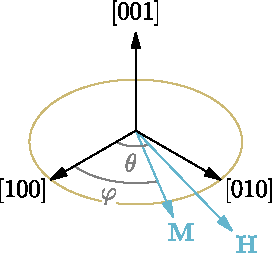
\includegraphics{figures/disk_001.pdf}
    \caption{\itshape Disco de hierro cortado en el plano (100).}
    \label{fig:disk_001}
  \end{marginfigure}

  Notando que la magnetización también estará en el plano (100),
  tenemos la situación de la figura \ref{fig:disk_001}. La energía de
  anisotropía de un cristal cúbico viene dada por
  \begin{equation}
    U_k = k_1 (α_1^2α_2^2 + α_2^2α_3^2 + α_3^2α_1^2) + k_2 α_1^2 α_2^2 α_3^2
  \end{equation}
  donde $α_i$ son los cosenos de $\symbf{M}$ con los ejes
  cristalográficos, que en este caso coinciden con los ejes de
  coordenadas del dibujo. Se tiene:
  \begin{equation}
    \begin{split}
      α_1 &= \cos φ \\
      α_2 &=\sin φ \\
      α_3 &= \cos 90 = 0
    \end{split}
  \end{equation}
  Con estos $α_i$, la energía de anisotropía queda como
  \begin{equation}
    U_k = k_1(\cos^2φ\sin^2φ) = \frac{k_1}{8}(1-\cos 4φ)
  \end{equation}
  Por otra parte, tenemos la energía magnética del material, calculable como
  \begin{equation}
    U\sub{H} = - \symbf{M}\symbf{M} = -MH\cos(θ-φ)
  \end{equation}
  En equilibrio no debe haber par de fuerzas. Como éste se define por
  $\pdv{U\sub{T}}{φ}$, donde $U\sub{T} = U_k + U\sub{H}$, obtenemos
  \begin{equation}
    \frac{k_1}{2} \sin 4φ = MH\sin(θ-φ)
  \end{equation}

\begin{tcolorbox}[halign=left]
  \emph{
    Obtener el par de fuerzas.
  }
\end{tcolorbox}

Suponemos un campo $H$ muy grande, de forma que $\symbf{M}=\symbf{H}$
y por lo tanto $φ=θ$. Las energías quedan como
\begin{align}
  U_k &= k_1(\cos^2θ\sin^2θ) = \frac{k_1}{8}(1-\cos4θ) \\
  U\sub{H} &= -HM
\end{align}
El par será
\begin{equation}
  T = -\pdv{(U_k+U\sub{H})}{θ} = \frac{k_1}{2} \sin 4θ
\end{equation}

\begin{tcolorbox}[halign=left]
  \emph{
    Obtener el par de fuerzas si el disco se corta con la superficie
    en el plano $(110)$.
  }
\end{tcolorbox}

\begin{marginfigure}
  \centering
  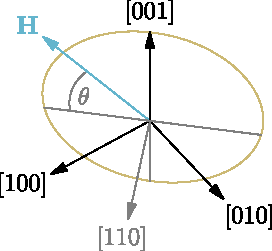
\includegraphics{figures/disk_110.pdf}
  \caption{\itshape Disco de hierro cortado en el plano (110). Se
    supone un $H$ suficientemente elevado como para que
    $\symbf{M}=\symbf{H}$.}
  \label{fig:disk_001}
\end{marginfigure}

La situación es la de la figura \ref{fig:disk_001}; idéntica salvo por
que hemos girado \SI{90}{\degree} en el eje [100] y \SI{45}{\degree}
en el eje [001]. De nuevo, suponemos un campo $\symbf{H}=\symbf{B}$.

Notamos que los ejes con los que hay que calcular los cosenos directores
no son los mismos, así que giramos $(α_1\ α_2\ α_3)^\mathit{T}$ junto
al sistema con dos matrices de rotación:
\begin{equation}
  \symbf{α}' =
  \mqty(
    \cos 45 & -\sin 45& \\
    \sin 45 & \cos 45 &\\
            &         & 1\\
  )
  \mqty(
  1 & & \\
    & \cos 90 & -\sin 90 \\
    & \sin 90 & \cos 90 \\
  )
  \mqty (\cos φ \\ 0 \\ \sin φ) =
  \frac{1}{\sqrt{2}}\mqty(\cos φ \\ \cos φ \\ \sqrt{2}\sin φ)
\end{equation}

Recalculamos la energía de anisotropía:
\begin{equation}
  \begin{split}
    U_k &= k_1 \left( \frac{\cos^2}{2}\frac{\cos^2}{2} +
      \frac{2\cos^2θ}{2} \sin^2θ \right) + k_2 \frac{\cos^2θ}{2} \sin^2 θ \\
    &= \frac{k_1}{4} (\cos^4θ + 4\cos^2θ \sin^2θ) + \frac{k_2}{2}
    \cos^2θ \sin^2θ
  \end{split}
\end{equation}
\begin{equation}
  U\sub{H} = -MH
\end{equation}
Y hallamos el par de fuerzas ($U\sub{H}$ sigue siendo $-MH$) como
\begin{equation}
  \begin{split}
    T &= - \pdv{U}{θ} = \frac{-k_1}{4}(4\sin θ \cos^3θ - 8\sin^3 θ\cos
    θ)\\  &- \frac{k_2}{2}(2\sinθ \cos^2θ - 2\sin^3θ \cos^3θ)
  \end{split}
\end{equation}

% 3.6
\begin{tcolorbox}[halign=left]
  \lettrine[lines=2]{\color{blue!50!white}3.6}{}
  \emph{
    Demostrar que bajo un esfuerzo $σ$ un material ferromagnético verifica
    }
    \begin{equation*}
      \frac{1}{ℓ} \left( \pdv{ℓ}{H} \right) = \left( \pdv{M}{σ} \right)_H
    \end{equation*}
    \emph{donde $ℓ$ es la longitud del espécimen.}
\end{tcolorbox}

La energía libre de Gibbs se define como
\begin{equation}
  \begin{split}
    G &= \mathcal{E} - TS \\
                &= U - HM -σ \int \dd{\nicefrac{δℓ}{ℓ}}  - TS
  \end{split}
\end{equation}
con $\mathcal{E}$ la entalpía, $U$ es la energía interna y $S$ la
entropía. A temperatura constante, diferenciamos empleando
\textit{heavily} la regla de la cadena
\begin{equation}
  \begin{split}
    \dd{G} &= dU - H \dd{M} - M \dd{H}- \dd{σ}\frac{δℓ}{ℓ} - σ
    \cancelto{∼0}{\dd[2]{ \frac{δℓ}{ℓ}}} - T \dd{S} \\
    &= -M \dd{H} - \frac{δℓ}{ℓ} \dd{σ}
  \end{split}
\end{equation}
donde se ha usado que $\dd{U}=T \dd{S}+ H \dd{M}$. Como $-\dd{G}$ es un
diferencial exacto\footnote{
  En 1D, significaría que se puede definir la integral. En 2D, viene a
  significar que dado un diferencial $\dd{Q} = A \dd{x} + B \dd{y}$ se
  cumple que $\frac{\partial^2 Q}{\partial x \partial y} =
  \frac{\partial^2 Q}{\partial y \partial x}$ y en particular
  \begin{equation*}
    \left( \pdv{A}{y} \right)_{\mathclap{x}} = \left( \pdv{B}{x} \right)_{\mathclap{z}}
  \end{equation*}
}
obtenemos que
\begin{equation}
  \left( \pdv{M}{σ} \right)_H = \frac{1}{ℓ} \left( \pdv{ℓ}{H} \right)_σ
\end{equation}
Q.E.D.

% 3.7
\begin{tcolorbox}[halign=left]
  \lettrine[lines=2]{\color{blue!50!white}3.7}{}
  \emph{
    An electromagnet is designed with an air gap and pole faces
    geometry in order to optimize the magnetic field produced by the
    system when magnetised with magnetization $M$. One of the
    optimizing configurations is based on the use of truncated cone
    pole faces with the vertices in the middle of the air gap. Obtain
    the magnetic field produced in the center of the electromagnet and
    demonstrate that the cone angle $θ = 54^\circ 44'$ produces the
    maximum magnetic field.
    }
\end{tcolorbox}
\marginnote{
  \begin{center}
    
\includegraphics[width=2cm]{figures/flag.pdf}
  \end{center}
}

From the magnetization $M$ both a surface density and a volume density
arise, given by $ρ =∇ \mathbf{M}$ and $σ = \mathbf{M} \hat{n}$. The
magnetic field $H_x$ in the center of the poles is given by
\begin{equation*}
  H_x = 2\iiint \frac{ρ}{r^2} \cos α \dd{V} = 2 \iiint \frac{∇
    \mathbf{M}}{r^2} \cos α\dd{V}
\end{equation*}
where the 2 indicates that we are integrating only over one of the
pieces and $α∈[-θ,θ]$ is the angle subtended with the axis of the
piece by the line from the center of the air gap to the $\dd{V}$. We
can use the divergence theorem to reduce the previous integral to
\begin{equation*}
  H_x = 2 \iint \frac{\mathbf{M} \hat{n}}{r^2} \cos α \dd{S}
\end{equation*}
where $\dd{S}$ spans both $S_1$ and $S_2$ (figure \ref{fig:geom}). We
can neglect the rest of the piece because of the rapid fall of $H_x$
with $r$.

\begin{marginfigure}
  \centering
  \begin{tikzpicture}
    \draw[thin, gray] (0,0) -- (1.5,-1.5);
    \draw[<->, thin] (1,-1.5) -- (1.5,-1.5) node [below, midway] {$x$};
    \draw[|->, thin] (0.75,-1.5) -- (0.75,-1) node [left, midway] {$a$};
    \draw[|->, thin] (0,-1.5) -- (0,-0.15) node [left, midway] {$b$};
    \draw[thin] (1.25,-1.5) arc (180:135:0.25);
    \draw[thick] (0,0) -- (1,-1) -- (1,-2) -- (0,-3);
    \draw[thick,gray] (0,0) -- (-2,0);
    \draw[thick,gray] (0,-3) -- (-2,-3);
    \node at (0.8,-1.7) {$S_1$};
    \node at (0.7,-0.4) {$S_2$};
  \end{tikzpicture}
  \caption{\itshape Drawing of one of the truncated cone pieces. The
    piece's $θ$ angle is shown.}
  \label{fig:geom}
\end{marginfigure}

For the surface $S_1$, we have $\mathbf{M}\hat{n} = M$ and $r^2 = x^2
/ \cos^2 α$, with $\dd{S_1} = 2π y \dd{y}$ and $y = x \tan α$:
\begin{equation*}
  \begin{split}
    H_x^{S_1} &= \iint \frac{\mathbf{M}\hat{n}}{r^2} \cos α \dd{S_1}
    = \iint \frac{M}{x^2} \cos ^2 α \cos α \dd{S_1} \\
    &= \iint \frac{M}{x^2} \cos ^2 α \cos α 2π y \dd{y} = \int_0^θ
    \frac{M}{x^2} \cancel{\cos ^2 α} \cos α 2π y \frac{x \dd{α}}{\cancel{\cos^2 α}} \\
    &= 2πM \int_0^θ \frac{1}{x} y \cos α \dd{α} = 2πM \int_0^θ \sin α \dd{α}
    = 2π M (1 -\cos θ)
  \end{split}
\end{equation*}


For the surface $S_2$, $\mathbf{M}\hat{n} = M \sin θ$ and $\dd{S_2} =
\frac{2π ζ }{\sin θ} \dd{ζ}$, with $r^2 = ζ^2 / \sin^2 θ$ and $α =
θ$.
\marginnote{$ζ∈[a,b]$ is a height from the axis of the piece to the
side $S_2$.}
\begin{equation*}
  \begin{split}
    H_x^{S_2} &= \iint \frac{\mathbf{M}\hat{n}}{r^2} \cos α \dd{S_2}
    = \iint \frac{M \sin θ}{ζ^2} \sin^2 α \cos α \dd{S_2} \\
    &= \int _a^b \frac{M \sin θ}{ζ^2} \sin^2 α \cos α  \frac{2πζ}{\sin θ} \dd{ζ}
    = \int _a^b \frac{M \sin θ}{ζ^2} \sin^2 θ \cos θ \frac{2πζ}{\sin θ}
    \dd{ζ} \\
    &= 2πM\sin^2θ \cos θ\int _a^b \frac{\dd{ζ}}{ζ} = 2π M \sin^2 θ \cos θ
    \log \frac{b}{a}
  \end{split}
\end{equation*}

\begin{marginfigure}
  \centering
  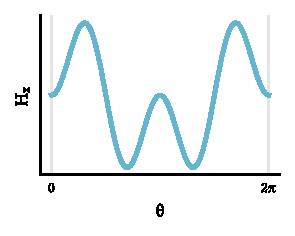
\includegraphics{figures/sineplot.pdf}
  \caption{\itshape The field $H_x$ has a maximum at $θ ∼ \SI{55}{\degree}$ if we
    neglect the flat faces contribution to the field.}
  \label{fig:sineplot}
\end{marginfigure}
Adding both integrals and multiplying by the two poles, we obtain
\begin{equation*}
  \boxed{
    H_x = 4πM \left( 1 - \cos θ + \sin^2 θ \cos θ \log \frac{b}{a} \right)
  }
\end{equation*}
If we neglect the contribution of the flat faces ($1-\cos θ$), we
find that the maximum of $H_x$ is, like the formulation proposes, $θ =
54^\circ 44'$. If we don't neglect it, the maximum is a function of $a/b$.

\begin{tcolorbox}[halign=left]
  \lettrine[lines=2]{\color{blue!50!white}3.8}{}
  \emph{
    Obtener los índices $(hkl)$ para las reflexiones permitidas en
    una red FCC de MnO, que es antiferromagnético por debajo de
    $T\sub{N}=\SI{122}{\kelvin}$ y tiene un tamaño de celda
    $a=\SI{4.43}{\angstrom}$.
    }
\end{tcolorbox}

Las posiciones de los átomos de la red se expresan como
\begin{equation}
  \symbf{r}_{j} = u_j \symbf{a}_1 + v_j \symbf{a}_2 + w_j \symbf{a}_3
\end{equation}
donde los $\symbf{a}_i$ son los vectores primitivos de la red. En una
FCC, tenemos una base dada por
\begin{equation}
  (u_j\ v_j\ w_j) ∈ \{\ (0\ 0\ 0),\ (\oh\ \oh\ 0),\ (\oh\ 0\ \oh),\ (0\ \oh\ \oh)\  \ \}
\end{equation}
Sabiendo que la intensidad de los picos de difracción es proporcional
al factor de estructura al cuadrado, tratamos de ver donde éste se
anula:
\begin{equation}
  \begin{split}
    F(h,k,l)
    &= \sum_{j} f_j e^{2πi(hu_j+kv_j+lw_j)}\\
    &∝ 1 + e^{iπ(h+k)} + e^{iπ(h+l)} + e^{iπ(k+l)}
  \end{split}
\end{equation}
supuesto $f_\mathit{Mn} = f_\mathit{O}$. Sólo es no nulo si los
$h,k,l$ son todos pares o impares.

\begin{tcolorbox}[halign=left]
  \emph{
    Interpretar los patrones de difracción de neutrones (figura
    \ref{fig:diffract}) conociendo que se ha utilizado
    $λ=\SI{1.06}{\angstrom}$.
    }
\end{tcolorbox}

\begin{figure*}[!h]
  \centering
  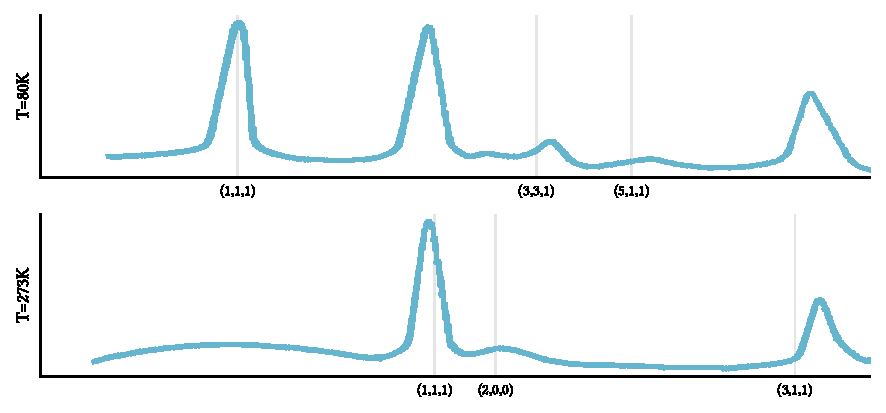
\includegraphics{figures/difract.pdf}
  \caption{\itshape Patrones de difracción para una red de MnO por
    encima y debajo de su temperatura de Neel. Se han marcado las
    predicciones de la ley de Bragg para los planos cristalográficos
    en el eje $x$.}
  \label{fig:diffract}
\end{figure*}

Partimos de la ley de Bragg, $nλ=2d\sin θ$. La distancia entre planos
de una red cúbica viene dada por $d=2π\abs{G}^{-1}=a^{-1}\sqrt{h^2+k^2+l^2}$;
sustituyendo $d$ en la ley de Bragg se obtiene
\begin{equation}
  \sin θ = \frac{λ}{2a} \sqrt{h^2+k^2+l^2}
  \label{eq:robin}
\end{equation}
donde se ha supuesto $n=1$. Como podemos comprobar en la figura, a
$T=\SI{273}{\kelvin}$ (por encima de la temperatura de Neel) se marcan
mucho los planos (111), (200) y (311). Que la intensidad de los picos
con todos los índices pares sea mucho mayor que la de los picos con
todos los índices impares nos indica\footnote{Criterio de autoridad.}
que $f_\mathit{Mn}$ y $f_\mathit{O}$ tienen signos opuestos.

Por debajo de la temperatura de Neel, hipotetizamos una celda unidad
el doble de grande que la química, y empleamos $2a$ en lugar de $a$ en
la ecuación \eqref{eq:robin}. Con ello, se obtiene que los picos
corresponden a un nuevo (111) y a los planos (311) y (511); los picos de la celda
química permanecen. Concluímos que la estructura magnética del MnO
consiste en láminas (111) paralelas, con todos los espines \textit{up}
y \textit{down} de forma alterna.

\end{document}
